% Options for packages loaded elsewhere
\PassOptionsToPackage{unicode}{hyperref}
\PassOptionsToPackage{hyphens}{url}
\documentclass[
]{article}
\usepackage{xcolor}
\usepackage[margin=1in]{geometry}
\usepackage{amsmath,amssymb}
\setcounter{secnumdepth}{-\maxdimen} % remove section numbering
\usepackage{iftex}
\ifPDFTeX
  \usepackage[T1]{fontenc}
  \usepackage[utf8]{inputenc}
  \usepackage{textcomp} % provide euro and other symbols
\else % if luatex or xetex
  \usepackage{unicode-math} % this also loads fontspec
  \defaultfontfeatures{Scale=MatchLowercase}
  \defaultfontfeatures[\rmfamily]{Ligatures=TeX,Scale=1}
\fi
\usepackage{lmodern}
\ifPDFTeX\else
  % xetex/luatex font selection
\fi
% Use upquote if available, for straight quotes in verbatim environments
\IfFileExists{upquote.sty}{\usepackage{upquote}}{}
\IfFileExists{microtype.sty}{% use microtype if available
  \usepackage[]{microtype}
  \UseMicrotypeSet[protrusion]{basicmath} % disable protrusion for tt fonts
}{}
\makeatletter
\@ifundefined{KOMAClassName}{% if non-KOMA class
  \IfFileExists{parskip.sty}{%
    \usepackage{parskip}
  }{% else
    \setlength{\parindent}{0pt}
    \setlength{\parskip}{6pt plus 2pt minus 1pt}}
}{% if KOMA class
  \KOMAoptions{parskip=half}}
\makeatother
\usepackage{color}
\usepackage{fancyvrb}
\newcommand{\VerbBar}{|}
\newcommand{\VERB}{\Verb[commandchars=\\\{\}]}
\DefineVerbatimEnvironment{Highlighting}{Verbatim}{commandchars=\\\{\}}
% Add ',fontsize=\small' for more characters per line
\usepackage{framed}
\definecolor{shadecolor}{RGB}{248,248,248}
\newenvironment{Shaded}{\begin{snugshade}}{\end{snugshade}}
\newcommand{\AlertTok}[1]{\textcolor[rgb]{0.94,0.16,0.16}{#1}}
\newcommand{\AnnotationTok}[1]{\textcolor[rgb]{0.56,0.35,0.01}{\textbf{\textit{#1}}}}
\newcommand{\AttributeTok}[1]{\textcolor[rgb]{0.13,0.29,0.53}{#1}}
\newcommand{\BaseNTok}[1]{\textcolor[rgb]{0.00,0.00,0.81}{#1}}
\newcommand{\BuiltInTok}[1]{#1}
\newcommand{\CharTok}[1]{\textcolor[rgb]{0.31,0.60,0.02}{#1}}
\newcommand{\CommentTok}[1]{\textcolor[rgb]{0.56,0.35,0.01}{\textit{#1}}}
\newcommand{\CommentVarTok}[1]{\textcolor[rgb]{0.56,0.35,0.01}{\textbf{\textit{#1}}}}
\newcommand{\ConstantTok}[1]{\textcolor[rgb]{0.56,0.35,0.01}{#1}}
\newcommand{\ControlFlowTok}[1]{\textcolor[rgb]{0.13,0.29,0.53}{\textbf{#1}}}
\newcommand{\DataTypeTok}[1]{\textcolor[rgb]{0.13,0.29,0.53}{#1}}
\newcommand{\DecValTok}[1]{\textcolor[rgb]{0.00,0.00,0.81}{#1}}
\newcommand{\DocumentationTok}[1]{\textcolor[rgb]{0.56,0.35,0.01}{\textbf{\textit{#1}}}}
\newcommand{\ErrorTok}[1]{\textcolor[rgb]{0.64,0.00,0.00}{\textbf{#1}}}
\newcommand{\ExtensionTok}[1]{#1}
\newcommand{\FloatTok}[1]{\textcolor[rgb]{0.00,0.00,0.81}{#1}}
\newcommand{\FunctionTok}[1]{\textcolor[rgb]{0.13,0.29,0.53}{\textbf{#1}}}
\newcommand{\ImportTok}[1]{#1}
\newcommand{\InformationTok}[1]{\textcolor[rgb]{0.56,0.35,0.01}{\textbf{\textit{#1}}}}
\newcommand{\KeywordTok}[1]{\textcolor[rgb]{0.13,0.29,0.53}{\textbf{#1}}}
\newcommand{\NormalTok}[1]{#1}
\newcommand{\OperatorTok}[1]{\textcolor[rgb]{0.81,0.36,0.00}{\textbf{#1}}}
\newcommand{\OtherTok}[1]{\textcolor[rgb]{0.56,0.35,0.01}{#1}}
\newcommand{\PreprocessorTok}[1]{\textcolor[rgb]{0.56,0.35,0.01}{\textit{#1}}}
\newcommand{\RegionMarkerTok}[1]{#1}
\newcommand{\SpecialCharTok}[1]{\textcolor[rgb]{0.81,0.36,0.00}{\textbf{#1}}}
\newcommand{\SpecialStringTok}[1]{\textcolor[rgb]{0.31,0.60,0.02}{#1}}
\newcommand{\StringTok}[1]{\textcolor[rgb]{0.31,0.60,0.02}{#1}}
\newcommand{\VariableTok}[1]{\textcolor[rgb]{0.00,0.00,0.00}{#1}}
\newcommand{\VerbatimStringTok}[1]{\textcolor[rgb]{0.31,0.60,0.02}{#1}}
\newcommand{\WarningTok}[1]{\textcolor[rgb]{0.56,0.35,0.01}{\textbf{\textit{#1}}}}
\usepackage{graphicx}
\makeatletter
\newsavebox\pandoc@box
\newcommand*\pandocbounded[1]{% scales image to fit in text height/width
  \sbox\pandoc@box{#1}%
  \Gscale@div\@tempa{\textheight}{\dimexpr\ht\pandoc@box+\dp\pandoc@box\relax}%
  \Gscale@div\@tempb{\linewidth}{\wd\pandoc@box}%
  \ifdim\@tempb\p@<\@tempa\p@\let\@tempa\@tempb\fi% select the smaller of both
  \ifdim\@tempa\p@<\p@\scalebox{\@tempa}{\usebox\pandoc@box}%
  \else\usebox{\pandoc@box}%
  \fi%
}
% Set default figure placement to htbp
\def\fps@figure{htbp}
\makeatother
\setlength{\emergencystretch}{3em} % prevent overfull lines
\providecommand{\tightlist}{%
  \setlength{\itemsep}{0pt}\setlength{\parskip}{0pt}}
\usepackage{bookmark}
\IfFileExists{xurl.sty}{\usepackage{xurl}}{} % add URL line breaks if available
\urlstyle{same}
\hypersetup{
  pdftitle={Final Project Study},
  pdfauthor={Zeynep TUTAR},
  hidelinks,
  pdfcreator={LaTeX via pandoc}}

\title{Final Project Study}
\author{Zeynep TUTAR}
\date{}

\begin{document}
\maketitle

\begin{Shaded}
\begin{Highlighting}[]
\FunctionTok{library}\NormalTok{(readxl)  }\CommentTok{\#for reading excel}
\FunctionTok{library}\NormalTok{(lmtest)  }\CommentTok{\#for the use of DW test, autocorrelation check}
\FunctionTok{library}\NormalTok{(forecast)  }\CommentTok{\#for linear reg for time series}
\FunctionTok{library}\NormalTok{(DIMORA)  }\CommentTok{\#for innovation dif models (GBM, Bass Model etc.)}
\FunctionTok{library}\NormalTok{(naniar)}
\FunctionTok{library}\NormalTok{(ggplot2)}
\FunctionTok{library}\NormalTok{(corrplot)}
\FunctionTok{library}\NormalTok{(car)}
\FunctionTok{library}\NormalTok{(dplyr)}
\FunctionTok{library}\NormalTok{(tidyr)}
\FunctionTok{library}\NormalTok{(prophet)}
\FunctionTok{library}\NormalTok{(Metrics)}
\FunctionTok{library}\NormalTok{(MLmetrics)}
\end{Highlighting}
\end{Shaded}

\section{1) Data Exploration \&
Preprocessing}\label{data-exploration-preprocessing}

\subsection{Load and Inspect the
Dataset}\label{load-and-inspect-the-dataset}

\begin{Shaded}
\begin{Highlighting}[]
\NormalTok{ott\_cinema\_monthly }\OtherTok{\textless{}{-}} \FunctionTok{read\_excel}\NormalTok{(}\StringTok{"ott\_cinema\_dataset.xlsx"}\NormalTok{, }\AttributeTok{sheet =} \StringTok{"Monthly"}\NormalTok{)}
\FunctionTok{str}\NormalTok{(ott\_cinema\_monthly)}
\end{Highlighting}
\end{Shaded}

\begin{verbatim}
tibble [216 x 9] (S3: tbl_df/tbl/data.frame)
 $ Time                    : chr [1:216] "2006-01" "2006-02" "2006-03" "2006-04" ...
 $ cinema_admissions       : num [1:216] 13700979 8207270 10102967 10872037 9408449 ...
 $ cinema_screenings       : num [1:216] 120005 102136 109564 110636 103219 ...
 $ cinema_audience_spending: num [1:216] 89522221 50597282 61407884 68866213 58029889 ...
 $ cinema_avg_spending_pp  : num [1:216] 6.53 6.16 6.08 6.33 6.17 ...
 $ gooogle_trend_ott       : num [1:216] 0 0 0 0 0 0 0 0 0 0 ...
 $ cpi_all                 : num [1:216] 0.2 0.2 0.2 0.3 0.2 0.2 0.4 0.2 -0.1 -0.2 ...
 $ cpi_culture             : num [1:216] 0.6 -0.2 0.2 -0.2 -0.1 0.1 0.4 0.7 0.2 -0.6 ...
 $ covid_cases             : num [1:216] 0 0 0 0 0 0 0 0 0 0 ...
\end{verbatim}

\begin{Shaded}
\begin{Highlighting}[]
\NormalTok{ott\_cinema\_annual }\OtherTok{\textless{}{-}} \FunctionTok{read\_excel}\NormalTok{(}\StringTok{"ott\_cinema\_dataset.xlsx"}\NormalTok{, }\AttributeTok{sheet =} \StringTok{"Annual"}\NormalTok{)}
\FunctionTok{str}\NormalTok{(ott\_cinema\_annual)}
\end{Highlighting}
\end{Shaded}

\begin{verbatim}
tibble [18 x 4] (S3: tbl_df/tbl/data.frame)
 $ Year               : num [1:18] 2006 2007 2008 2009 2010 ...
 $ ott_subscriptions_M: num [1:18] 0 0 0 0 0 0 0 0 0.3 0.8 ...
 $ ott_spending_M_EUR : num [1:18] 0 0 0.6 0.7 1.4 9.5 21.9 21.1 39 64.1 ...
 $ cinema_admissions  : num [1:18] 1.06e+08 1.17e+08 1.12e+08 1.11e+08 1.23e+08 ...
\end{verbatim}

\begin{Shaded}
\begin{Highlighting}[]
\CommentTok{\# ott\_cinema\_monthly$Time=as.Date(paste0(ott\_cinema\_monthly$Time,}
\CommentTok{\# \textquotesingle{}{-}01\textquotesingle{}), format = \textquotesingle{}\%Y{-}\%m{-}\%d\textquotesingle{}) ott\_cinema\_annual$Year \textless{}{-}}
\CommentTok{\# as.Date(paste0(ott\_cinema\_annual$Year, \textquotesingle{}{-}01{-}01\textquotesingle{}), format=\textquotesingle{}\%Y{-}\%m{-}\%d\textquotesingle{})}
\end{Highlighting}
\end{Shaded}

\begin{Shaded}
\begin{Highlighting}[]
\CommentTok{\# Check for missing values}
\NormalTok{ott\_cinema\_monthly[}\FunctionTok{apply}\NormalTok{(}\FunctionTok{is.na}\NormalTok{(ott\_cinema\_monthly), }\DecValTok{1}\NormalTok{, any), ]}
\end{Highlighting}
\end{Shaded}

\begin{verbatim}
# A tibble: 19 x 9
   Time    cinema_admissions cinema_screenings cinema_audience_spending
   <chr>               <dbl>             <dbl>                    <dbl>
 1 2013-01                NA                NA                      NA 
 2 2013-02                NA                NA                      NA 
 3 2013-03                NA                NA                      NA 
 4 2013-04                NA                NA                      NA 
 5 2013-05                NA                NA                      NA 
 6 2013-06                NA                NA                      NA 
 7 2013-07                NA                NA                      NA 
 8 2013-08                NA                NA                      NA 
 9 2013-09                NA                NA                      NA 
10 2013-10                NA                NA                      NA 
11 2013-11                NA                NA                      NA 
12 2013-12                NA                NA                      NA 
13 2020-04                 0                 0                     326.
14 2020-05                 0                 0                     198 
15 2020-11                 0                 0                    4824.
16 2020-12                 0                 0                   56332 
17 2021-01                 0                 0                   27483 
18 2021-02                 0                 0                   14354.
19 2021-03                 0                 0                    2165.
# i 5 more variables: cinema_avg_spending_pp <dbl>, gooogle_trend_ott <dbl>,
#   cpi_all <dbl>, cpi_culture <dbl>, covid_cases <dbl>
\end{verbatim}

\begin{Shaded}
\begin{Highlighting}[]
\FunctionTok{vis\_miss}\NormalTok{(ott\_cinema\_monthly)}
\end{Highlighting}
\end{Shaded}

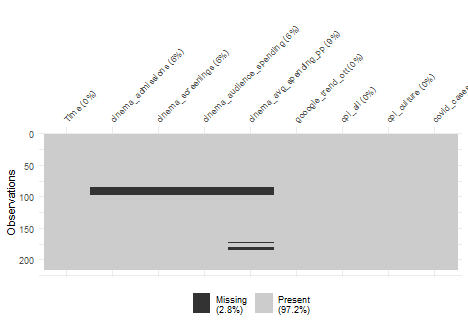
\includegraphics[width=0.8\linewidth]{plots/missing_visual-1}

\begin{Shaded}
\begin{Highlighting}[]
\NormalTok{ott\_cinema\_annual[}\FunctionTok{apply}\NormalTok{(}\FunctionTok{is.na}\NormalTok{(ott\_cinema\_annual), }\DecValTok{1}\NormalTok{, any), ]}
\end{Highlighting}
\end{Shaded}

\begin{verbatim}
# A tibble: 0 x 4
# i 4 variables: Year <dbl>, ott_subscriptions_M <dbl>,
#   ott_spending_M_EUR <dbl>, cinema_admissions <dbl>
\end{verbatim}

\begin{Shaded}
\begin{Highlighting}[]
\FunctionTok{vis\_miss}\NormalTok{(ott\_cinema\_annual)}
\end{Highlighting}
\end{Shaded}

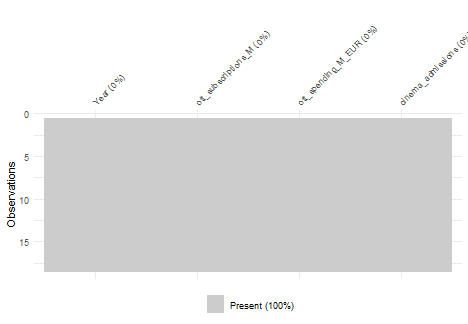
\includegraphics[width=0.8\linewidth]{plots/missing_visual-2}

\begin{Shaded}
\begin{Highlighting}[]
\NormalTok{ott\_cinema\_monthly.ts }\OtherTok{\textless{}{-}} \FunctionTok{ts}\NormalTok{(ott\_cinema\_monthly[, }\SpecialCharTok{{-}}\DecValTok{1}\NormalTok{], }\AttributeTok{start =} \FunctionTok{c}\NormalTok{(}\DecValTok{2006}\NormalTok{, }\DecValTok{1}\NormalTok{),}
    \AttributeTok{end =} \FunctionTok{c}\NormalTok{(}\DecValTok{2023}\NormalTok{, }\DecValTok{12}\NormalTok{), }\AttributeTok{frequency =} \DecValTok{12}\NormalTok{)}
\NormalTok{ott\_cinema\_annual.ts }\OtherTok{\textless{}{-}} \FunctionTok{ts}\NormalTok{(ott\_cinema\_annual[, }\SpecialCharTok{{-}}\DecValTok{1}\NormalTok{], }\AttributeTok{start =} \FunctionTok{c}\NormalTok{(}\DecValTok{2006}\NormalTok{), }\AttributeTok{end =} \FunctionTok{c}\NormalTok{(}\DecValTok{2023}\NormalTok{),}
    \AttributeTok{frequency =} \DecValTok{1}\NormalTok{)}
\end{Highlighting}
\end{Shaded}

\begin{Shaded}
\begin{Highlighting}[]
\FunctionTok{plot}\NormalTok{(ott\_cinema\_monthly.ts, }\AttributeTok{main =} \StringTok{"Monthly Cinema{-}OTT Dataset"}\NormalTok{, }\AttributeTok{cex.lab =} \FloatTok{0.45}\NormalTok{,}
    \AttributeTok{type =} \StringTok{"o"}\NormalTok{, }\AttributeTok{pch =} \DecValTok{16}\NormalTok{, }\AttributeTok{lty =} \DecValTok{3}\NormalTok{, }\AttributeTok{cex =} \FloatTok{0.6}\NormalTok{)}
\end{Highlighting}
\end{Shaded}

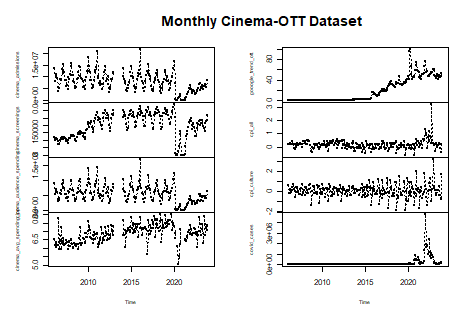
\includegraphics[width=0.8\linewidth]{plots/plot_monthly_raw-1}

\begin{Shaded}
\begin{Highlighting}[]
\FunctionTok{plot}\NormalTok{(ott\_cinema\_annual.ts, }\AttributeTok{main =} \StringTok{"Annual Cinema {-} OTT Dataset"}\NormalTok{, }\AttributeTok{cex.lab =} \FloatTok{0.45}\NormalTok{,}
    \AttributeTok{type =} \StringTok{"o"}\NormalTok{, }\AttributeTok{pch =} \DecValTok{16}\NormalTok{, }\AttributeTok{lty =} \DecValTok{3}\NormalTok{, }\AttributeTok{cex =} \FloatTok{0.6}\NormalTok{)}
\end{Highlighting}
\end{Shaded}

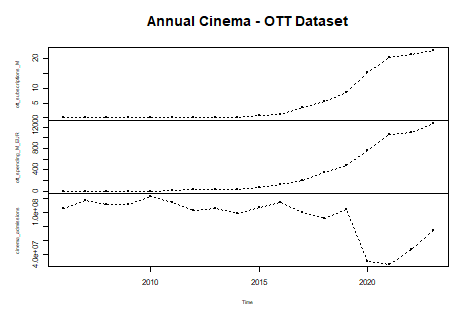
\includegraphics[width=0.8\linewidth]{plots/plot_annual_raw-1}

\subsection{Handle Missing Values}\label{handle-missing-values}

\subsubsection{Handle Monthly Dataset Missing
Values}\label{handle-monthly-dataset-missing-values}

\begin{Shaded}
\begin{Highlighting}[]
\CommentTok{\# Define the total annual values for 2013 for each column}
\NormalTok{total\_2013 }\OtherTok{\textless{}{-}} \FunctionTok{list}\NormalTok{(}\AttributeTok{cinema\_screenings =} \DecValTok{3014642}\NormalTok{, }\AttributeTok{cinema\_admissions =} \DecValTok{106124433}\NormalTok{,}
    \AttributeTok{cinema\_audience\_spending =} \FloatTok{732299026.82}\NormalTok{)}

\CommentTok{\# Define the columns to impute}
\NormalTok{columns\_to\_impute }\OtherTok{\textless{}{-}} \FunctionTok{c}\NormalTok{(}\StringTok{"cinema\_screenings"}\NormalTok{, }\StringTok{"cinema\_admissions"}\NormalTok{, }\StringTok{"cinema\_audience\_spending"}\NormalTok{,}
    \StringTok{"cinema\_avg\_spending\_pp"}\NormalTok{)}

\CommentTok{\# Create a copy of the time series object for imputation}
\NormalTok{cinema\_imputed }\OtherTok{\textless{}{-}}\NormalTok{ ott\_cinema\_monthly.ts}

\CommentTok{\# Filter data to include only 2011, 2012, 2014, 2015 for monthly}
\CommentTok{\# averages}
\NormalTok{selected\_years }\OtherTok{\textless{}{-}}\NormalTok{ (}\FunctionTok{time}\NormalTok{(ott\_cinema\_monthly.ts) }\SpecialCharTok{\textgreater{}=} \DecValTok{2011} \SpecialCharTok{\&} \FunctionTok{time}\NormalTok{(ott\_cinema\_monthly.ts) }\SpecialCharTok{\textless{}}
    \DecValTok{2013}\NormalTok{) }\SpecialCharTok{|}\NormalTok{ (}\FunctionTok{time}\NormalTok{(ott\_cinema\_monthly.ts) }\SpecialCharTok{\textgreater{}=} \DecValTok{2014} \SpecialCharTok{\&} \FunctionTok{time}\NormalTok{(ott\_cinema\_monthly.ts) }\SpecialCharTok{\textless{}}
    \DecValTok{2016}\NormalTok{)}
\end{Highlighting}
\end{Shaded}

\begin{Shaded}
\begin{Highlighting}[]
\CommentTok{\# Loop through each column to impute missing values}
\ControlFlowTok{for}\NormalTok{ (col }\ControlFlowTok{in}\NormalTok{ columns\_to\_impute) \{}
    \CommentTok{\# Extract the column data}
\NormalTok{    column\_data }\OtherTok{\textless{}{-}} \FunctionTok{as.numeric}\NormalTok{(ott\_cinema\_monthly.ts[, col])}

    \ControlFlowTok{if}\NormalTok{ (col }\SpecialCharTok{==} \StringTok{"cinema\_avg\_spending\_pp"}\NormalTok{) \{}
        \CommentTok{\# Calculate avg\_spending\_pp using the imputed}
        \CommentTok{\# audience\_spending/audience\_admissions}
\NormalTok{        imputed\_2013 }\OtherTok{\textless{}{-}}\NormalTok{ cinema\_imputed[, }\StringTok{"cinema\_audience\_spending"}\NormalTok{]}\SpecialCharTok{/}\NormalTok{cinema\_imputed[,}
            \StringTok{"cinema\_admissions"}\NormalTok{]}

        \CommentTok{\# Replace the missing 2013 data with the calculated values}
\NormalTok{        column\_data[}\FunctionTok{time}\NormalTok{(ott\_cinema\_monthly.ts) }\SpecialCharTok{\textgreater{}=} \DecValTok{2013} \SpecialCharTok{\&} \FunctionTok{time}\NormalTok{(ott\_cinema\_monthly.ts) }\SpecialCharTok{\textless{}}
            \DecValTok{2014}\NormalTok{] }\OtherTok{\textless{}{-}}\NormalTok{ imputed\_2013[}\FunctionTok{time}\NormalTok{(ott\_cinema\_monthly.ts) }\SpecialCharTok{\textgreater{}=} \DecValTok{2013} \SpecialCharTok{\&} \FunctionTok{time}\NormalTok{(ott\_cinema\_monthly.ts) }\SpecialCharTok{\textless{}}
            \DecValTok{2014}\NormalTok{]}

        \CommentTok{\# Handle missing values in 2020 and 2021 (due to COVID{-}19}
        \CommentTok{\# impact)}
\NormalTok{        column\_data[}\FunctionTok{time}\NormalTok{(ott\_cinema\_monthly.ts) }\SpecialCharTok{\textgreater{}=} \DecValTok{2020} \SpecialCharTok{\&} \FunctionTok{time}\NormalTok{(ott\_cinema\_monthly.ts) }\SpecialCharTok{\textless{}}
            \DecValTok{2021} \SpecialCharTok{\&} \FunctionTok{is.na}\NormalTok{(column\_data)] }\OtherTok{\textless{}{-}} \FloatTok{6.35}  \CommentTok{\# Average for 2020}
\NormalTok{        column\_data[}\FunctionTok{time}\NormalTok{(ott\_cinema\_monthly.ts) }\SpecialCharTok{\textgreater{}=} \DecValTok{2021} \SpecialCharTok{\&} \FunctionTok{time}\NormalTok{(ott\_cinema\_monthly.ts) }\SpecialCharTok{\textless{}}
            \DecValTok{2022} \SpecialCharTok{\&} \FunctionTok{is.na}\NormalTok{(column\_data)] }\OtherTok{\textless{}{-}} \FloatTok{6.76}  \CommentTok{\# Average for 2021}
\NormalTok{    \} }\ControlFlowTok{else}\NormalTok{ \{}
        \CommentTok{\# Handle cumulative features using selected years for}
        \CommentTok{\# proportions}
\NormalTok{        monthly\_proportions }\OtherTok{\textless{}{-}} \FunctionTok{colMeans}\NormalTok{(}\FunctionTok{matrix}\NormalTok{(column\_data[selected\_years],}
            \AttributeTok{ncol =} \DecValTok{12}\NormalTok{, }\AttributeTok{byrow =} \ConstantTok{TRUE}\NormalTok{), }\AttributeTok{na.rm =} \ConstantTok{TRUE}\NormalTok{)}
        \CommentTok{\# Normalize to proportions}
\NormalTok{        monthly\_proportions }\OtherTok{\textless{}{-}}\NormalTok{ monthly\_proportions}\SpecialCharTok{/}\FunctionTok{sum}\NormalTok{(monthly\_proportions)}
\NormalTok{        imputed\_2013 }\OtherTok{\textless{}{-}}\NormalTok{ monthly\_proportions }\SpecialCharTok{*}\NormalTok{ total\_2013[[col]]}

        \CommentTok{\# Replace the missing 2013 data with the imputed values}
\NormalTok{        column\_data[}\FunctionTok{time}\NormalTok{(ott\_cinema\_monthly.ts) }\SpecialCharTok{\textgreater{}=} \DecValTok{2013} \SpecialCharTok{\&} \FunctionTok{time}\NormalTok{(ott\_cinema\_monthly.ts) }\SpecialCharTok{\textless{}}
            \DecValTok{2014}\NormalTok{] }\OtherTok{\textless{}{-}}\NormalTok{ imputed\_2013}
\NormalTok{    \}}

    \CommentTok{\# Update the imputed data in the time series}
\NormalTok{    cinema\_imputed[, col] }\OtherTok{\textless{}{-}}\NormalTok{ column\_data}
\NormalTok{\}}
\end{Highlighting}
\end{Shaded}

\begin{Shaded}
\begin{Highlighting}[]
\CommentTok{\# Plot the original and imputed data for comparison}
\ControlFlowTok{for}\NormalTok{ (col }\ControlFlowTok{in}\NormalTok{ columns\_to\_impute) \{}
    \FunctionTok{par}\NormalTok{(}\AttributeTok{mfrow =} \FunctionTok{c}\NormalTok{(}\DecValTok{2}\NormalTok{, }\DecValTok{1}\NormalTok{), }\AttributeTok{mar =} \FunctionTok{c}\NormalTok{(}\DecValTok{4}\NormalTok{, }\DecValTok{4}\NormalTok{, }\DecValTok{2}\NormalTok{, }\DecValTok{1}\NormalTok{))}

    \CommentTok{\# Plot the original data}
    \FunctionTok{plot}\NormalTok{(ott\_cinema\_monthly.ts[, col], }\AttributeTok{type =} \StringTok{"o"}\NormalTok{, }\AttributeTok{pch =} \DecValTok{16}\NormalTok{, }\AttributeTok{lty =} \DecValTok{3}\NormalTok{, }\AttributeTok{cex =} \FloatTok{0.4}\NormalTok{,}
        \AttributeTok{main =} \FunctionTok{paste}\NormalTok{(}\StringTok{"Original"}\NormalTok{, col), }\AttributeTok{xlab =} \StringTok{"Time"}\NormalTok{, }\AttributeTok{ylab =}\NormalTok{ col)}

    \CommentTok{\# Plot the imputed data}
    \FunctionTok{plot}\NormalTok{(cinema\_imputed[, col], }\AttributeTok{type =} \StringTok{"o"}\NormalTok{, }\AttributeTok{pch =} \DecValTok{16}\NormalTok{, }\AttributeTok{lty =} \DecValTok{3}\NormalTok{, }\AttributeTok{cex =} \FloatTok{0.4}\NormalTok{,}
        \AttributeTok{main =} \FunctionTok{paste}\NormalTok{(}\StringTok{"Imputed"}\NormalTok{, col), }\AttributeTok{xlab =} \StringTok{"Time"}\NormalTok{, }\AttributeTok{ylab =}\NormalTok{ col)}
\NormalTok{\}}
\end{Highlighting}
\end{Shaded}

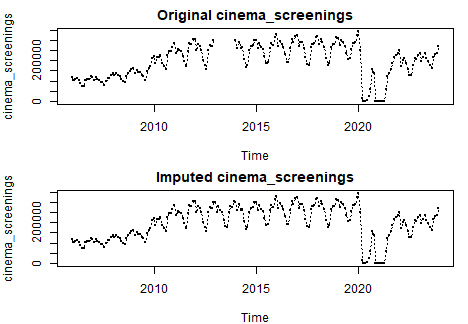
\includegraphics[width=0.5\linewidth]{plots/missing_vs_imputed-1}
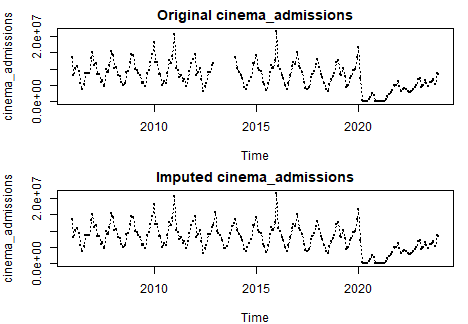
\includegraphics[width=0.5\linewidth]{plots/missing_vs_imputed-2}
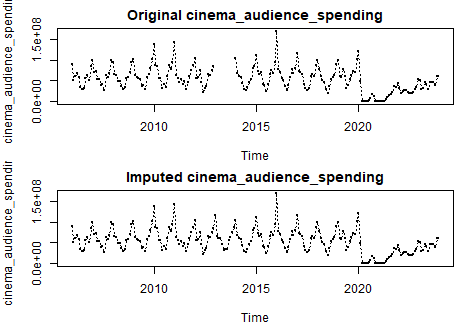
\includegraphics[width=0.5\linewidth]{plots/missing_vs_imputed-3}
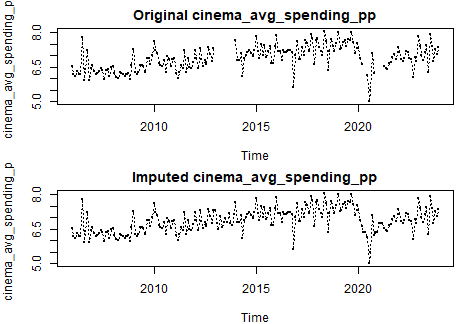
\includegraphics[width=0.5\linewidth]{plots/missing_vs_imputed-4}

\begin{Shaded}
\begin{Highlighting}[]
\FunctionTok{par}\NormalTok{(}\AttributeTok{mfrow =} \FunctionTok{c}\NormalTok{(}\DecValTok{1}\NormalTok{, }\DecValTok{1}\NormalTok{))}
\end{Highlighting}
\end{Shaded}

\begin{Shaded}
\begin{Highlighting}[]
\NormalTok{ott\_cinema\_monthly.ts }\OtherTok{\textless{}{-}}\NormalTok{ cinema\_imputed}
\NormalTok{ott\_cinema\_monthly }\OtherTok{\textless{}{-}} \FunctionTok{as.data.frame}\NormalTok{(cinema\_imputed)}

\CommentTok{\# Final plot of the imputed dataset}
\FunctionTok{plot}\NormalTok{(ott\_cinema\_monthly.ts, }\AttributeTok{main =} \StringTok{"Cinema{-}OTT Monthly Dataset (After Imputation)"}\NormalTok{,}
    \AttributeTok{cex.lab =} \FloatTok{0.45}\NormalTok{, }\AttributeTok{type =} \StringTok{"o"}\NormalTok{, }\AttributeTok{pch =} \DecValTok{16}\NormalTok{, }\AttributeTok{lty =} \DecValTok{3}\NormalTok{, }\AttributeTok{cex =} \FloatTok{0.6}\NormalTok{)}
\end{Highlighting}
\end{Shaded}

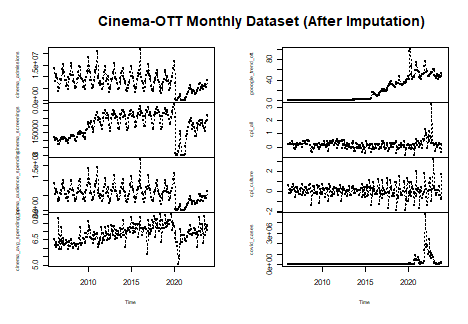
\includegraphics[width=0.8\linewidth]{plots/monthly_imputed-1}

\subsection{Collinearity Check}\label{collinearity-check}

\subsubsection{Correlation Matrix for Monthly
Data}\label{correlation-matrix-for-monthly-data}

\begin{Shaded}
\begin{Highlighting}[]
\CommentTok{\# Correlation Matrix for Monthly Data}
\NormalTok{ott\_cinema\_corr }\OtherTok{\textless{}{-}} \FunctionTok{as.data.frame}\NormalTok{(ott\_cinema\_monthly.ts)}

\CommentTok{\# Compute correlation matrix}
\NormalTok{cor\_matrix\_monthly }\OtherTok{\textless{}{-}} \FunctionTok{cor}\NormalTok{(ott\_cinema\_corr, }\AttributeTok{use =} \StringTok{"complete.obs"}\NormalTok{)}
\end{Highlighting}
\end{Shaded}

\begin{Shaded}
\begin{Highlighting}[]
\CommentTok{\# default\_margins \textless{}{-} par(\textquotesingle{}mar\textquotesingle{}) par(mar = c(5, 5, 4, 2) + 0.1)}

\CommentTok{\# Visualize correlation matrix}
\FunctionTok{corrplot}\NormalTok{(cor\_matrix\_monthly, }\AttributeTok{method =} \StringTok{"color"}\NormalTok{, }\AttributeTok{type =} \StringTok{"lower"}\NormalTok{, }\AttributeTok{tl.col =} \StringTok{"black"}\NormalTok{,}
    \AttributeTok{tl.srt =} \DecValTok{45}\NormalTok{, }\AttributeTok{addCoef.col =} \StringTok{"black"}\NormalTok{, }\AttributeTok{number.cex =} \FloatTok{0.8}\NormalTok{, }\AttributeTok{tl.cex =} \FloatTok{0.75}\NormalTok{)}
\end{Highlighting}
\end{Shaded}

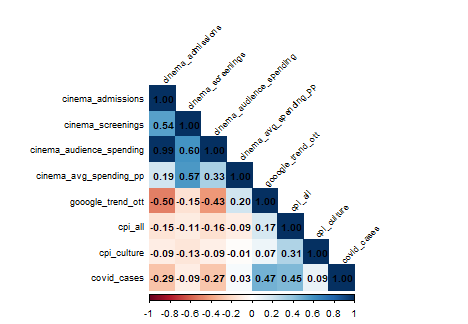
\includegraphics[width=0.8\linewidth]{plots/plot_corr_monthly-1}

\begin{Shaded}
\begin{Highlighting}[]
\CommentTok{\# title(main = \textquotesingle{}Correlation Matrix: Monthly Data\textquotesingle{}, line = 2, cex.main =}
\CommentTok{\# 1.2) par(mar = default\_margins)}
\end{Highlighting}
\end{Shaded}

\subsubsection{VIF Analysis for Monthly
Data}\label{vif-analysis-for-monthly-data}

\begin{Shaded}
\begin{Highlighting}[]
\CommentTok{\# Run VIF analysis Regression model with all predictors}
\NormalTok{vif\_model.monthly }\OtherTok{\textless{}{-}} \FunctionTok{lm}\NormalTok{(ott\_cinema\_monthly}\SpecialCharTok{$}\NormalTok{cinema\_admissions }\SpecialCharTok{\textasciitilde{}}\NormalTok{ . }\SpecialCharTok{{-}}\NormalTok{ ott\_cinema\_monthly}\SpecialCharTok{$}\NormalTok{cinema\_admissions,}
    \AttributeTok{data =}\NormalTok{ ott\_cinema\_monthly[, }\SpecialCharTok{{-}}\DecValTok{1}\NormalTok{])}
\CommentTok{\# Compute VIF}
\FunctionTok{vif}\NormalTok{(vif\_model.monthly)}
\end{Highlighting}
\end{Shaded}

\begin{verbatim}
       cinema_screenings cinema_audience_spending   cinema_avg_spending_pp 
                2.126995                 1.976895                 1.771816 
       gooogle_trend_ott                  cpi_all              cpi_culture 
                1.746757                 1.389224                 1.130118 
             covid_cases 
                1.578432 
\end{verbatim}

\begin{Shaded}
\begin{Highlighting}[]
\CommentTok{\# Compute correlation matrix cor\_matrix\_annual \textless{}{-}}
\CommentTok{\# cor(ott\_cinema\_annual[,{-}1], use = \textquotesingle{}complete.obs\textquotesingle{})}

\CommentTok{\# Visualize correlation matrix corrplot(cor\_matrix\_annual, method =}
\CommentTok{\# \textquotesingle{}color\textquotesingle{}, type = \textquotesingle{}lower\textquotesingle{}, tl.col = \textquotesingle{}black\textquotesingle{}, tl.srt = 45, addCoef.col =}
\CommentTok{\# \textquotesingle{}black\textquotesingle{}, number.cex = 0.65, , tl.cex=0.55) title(main = \textquotesingle{}Correlation}
\CommentTok{\# Matrix: Annual Data\textquotesingle{}, line = 2, cex.main = 1.2)}
\end{Highlighting}
\end{Shaded}

\subsubsection{Check correlation \& trends between OTT Data (Annual) and
Google Trends OTT
(Monthly)}\label{check-correlation-trends-between-ott-data-annual-and-google-trends-ott-monthly}

\begin{Shaded}
\begin{Highlighting}[]
\NormalTok{ott\_cinema\_monthly}\SpecialCharTok{$}\NormalTok{Year }\OtherTok{\textless{}{-}} \FunctionTok{rep}\NormalTok{(}\DecValTok{2006}\SpecialCharTok{:}\DecValTok{2023}\NormalTok{, }\AttributeTok{each =} \DecValTok{12}\NormalTok{)  }\CommentTok{\# Create a Year column}

\CommentTok{\# Aggregate Google Trends OTT monthly data to annual (sum)}
\NormalTok{google\_trends\_annual }\OtherTok{\textless{}{-}}\NormalTok{ ott\_cinema\_monthly }\SpecialCharTok{\%\textgreater{}\%}
    \FunctionTok{group\_by}\NormalTok{(Year) }\SpecialCharTok{\%\textgreater{}\%}
    \FunctionTok{summarise}\NormalTok{(}\AttributeTok{google\_trend\_ott =} \FunctionTok{sum}\NormalTok{(gooogle\_trend\_ott, }\AttributeTok{na.rm =} \ConstantTok{TRUE}\NormalTok{))}

\CommentTok{\# Merge with annual dataset}
\NormalTok{merged\_ott\_data }\OtherTok{\textless{}{-}} \FunctionTok{merge}\NormalTok{(ott\_cinema\_annual[, }\FunctionTok{c}\NormalTok{(}\DecValTok{1}\SpecialCharTok{:}\DecValTok{3}\NormalTok{)], google\_trends\_annual,}
    \AttributeTok{by.x =} \StringTok{"Year"}\NormalTok{, }\AttributeTok{by.y =} \StringTok{"Year"}\NormalTok{, }\AttributeTok{all.x =} \ConstantTok{TRUE}\NormalTok{)}
\end{Highlighting}
\end{Shaded}

\begin{Shaded}
\begin{Highlighting}[]
\CommentTok{\# Compute Correlation Matrix}
\NormalTok{cor\_matrix }\OtherTok{\textless{}{-}} \FunctionTok{cor}\NormalTok{(merged\_ott\_data[, }\SpecialCharTok{{-}}\DecValTok{1}\NormalTok{], }\AttributeTok{use =} \StringTok{"complete.obs"}\NormalTok{)}
\NormalTok{cor\_matrix}
\end{Highlighting}
\end{Shaded}

\begin{verbatim}
                    ott_subscriptions_M ott_spending_M_EUR google_trend_ott
ott_subscriptions_M           1.0000000          0.9980075        0.9379704
ott_spending_M_EUR            0.9980075          1.0000000        0.9344162
google_trend_ott              0.9379704          0.9344162        1.0000000
\end{verbatim}

\begin{Shaded}
\begin{Highlighting}[]
\CommentTok{\# Visualize Correlation Matrix corrplot(cor\_matrix, method = \textquotesingle{}color\textquotesingle{},}
\CommentTok{\# type = \textquotesingle{}lower\textquotesingle{}, tl.col = \textquotesingle{}black\textquotesingle{}, tl.srt = 45, addCoef.col = \textquotesingle{}black\textquotesingle{},}
\CommentTok{\# number.cex = 0.8, tl.cex=0.65)}
\end{Highlighting}
\end{Shaded}

\begin{Shaded}
\begin{Highlighting}[]
\NormalTok{min\_max\_scale }\OtherTok{\textless{}{-}} \ControlFlowTok{function}\NormalTok{(x) \{}
    \FunctionTok{return}\NormalTok{((x }\SpecialCharTok{{-}} \FunctionTok{min}\NormalTok{(x, }\AttributeTok{na.rm =} \ConstantTok{TRUE}\NormalTok{))}\SpecialCharTok{/}\NormalTok{(}\FunctionTok{max}\NormalTok{(x, }\AttributeTok{na.rm =} \ConstantTok{TRUE}\NormalTok{) }\SpecialCharTok{{-}} \FunctionTok{min}\NormalTok{(x, }\AttributeTok{na.rm =} \ConstantTok{TRUE}\NormalTok{)))}
\NormalTok{\}}

\CommentTok{\# Apply Min{-}Max Scaling to the relevant columns}
\NormalTok{merged\_ott\_data}\SpecialCharTok{$}\NormalTok{ott\_subscriptions\_scaled }\OtherTok{\textless{}{-}} \FunctionTok{min\_max\_scale}\NormalTok{(merged\_ott\_data}\SpecialCharTok{$}\NormalTok{ott\_subscriptions\_M)}

\NormalTok{merged\_ott\_data}\SpecialCharTok{$}\NormalTok{ott\_spending\_scaled }\OtherTok{\textless{}{-}} \FunctionTok{min\_max\_scale}\NormalTok{(merged\_ott\_data}\SpecialCharTok{$}\NormalTok{ott\_spending\_M\_EUR)}

\NormalTok{merged\_ott\_data}\SpecialCharTok{$}\NormalTok{google\_trend\_ott\_scaled }\OtherTok{\textless{}{-}} \FunctionTok{min\_max\_scale}\NormalTok{(merged\_ott\_data}\SpecialCharTok{$}\NormalTok{google\_trend\_ott)}
\end{Highlighting}
\end{Shaded}

\begin{Shaded}
\begin{Highlighting}[]
\CommentTok{\# Convert Year to Date format for better plotting merged\_ott\_data$Year}
\CommentTok{\# \textless{}{-} as.Date(paste0(merged\_ott\_data$Year, \textquotesingle{}{-}01{-}01\textquotesingle{}))}
\end{Highlighting}
\end{Shaded}

\begin{Shaded}
\begin{Highlighting}[]
\CommentTok{\# Compare trends}
\FunctionTok{plot}\NormalTok{(merged\_ott\_data}\SpecialCharTok{$}\NormalTok{Year, merged\_ott\_data}\SpecialCharTok{$}\NormalTok{ott\_subscriptions\_scaled, }\AttributeTok{type =} \StringTok{"l"}\NormalTok{,}
    \AttributeTok{col =} \StringTok{"blue"}\NormalTok{, }\AttributeTok{lwd =} \DecValTok{2}\NormalTok{, }\AttributeTok{xlab =} \StringTok{"Year"}\NormalTok{, }\AttributeTok{ylab =} \StringTok{"Normalized Value"}\NormalTok{, }\AttributeTok{main =} \StringTok{"OTT Subscriptions, OTT Spending, and Google Trends OTT"}\NormalTok{)}
\FunctionTok{lines}\NormalTok{(merged\_ott\_data}\SpecialCharTok{$}\NormalTok{Year, merged\_ott\_data}\SpecialCharTok{$}\NormalTok{ott\_spending\_scaled, }\AttributeTok{col =} \StringTok{"red"}\NormalTok{,}
    \AttributeTok{lwd =} \DecValTok{2}\NormalTok{)}
\FunctionTok{lines}\NormalTok{(merged\_ott\_data}\SpecialCharTok{$}\NormalTok{Year, merged\_ott\_data}\SpecialCharTok{$}\NormalTok{google\_trend\_ott\_scaled, }\AttributeTok{col =} \StringTok{"green"}\NormalTok{,}
    \AttributeTok{lwd =} \DecValTok{2}\NormalTok{)}
\FunctionTok{legend}\NormalTok{(}\StringTok{"topleft"}\NormalTok{, }\AttributeTok{legend =} \FunctionTok{c}\NormalTok{(}\StringTok{"OTT Subscriptions"}\NormalTok{, }\StringTok{"OTT Spending"}\NormalTok{, }\StringTok{"Google Trends OTT"}\NormalTok{),}
    \AttributeTok{col =} \FunctionTok{c}\NormalTok{(}\StringTok{"blue"}\NormalTok{, }\StringTok{"red"}\NormalTok{, }\StringTok{"green"}\NormalTok{), }\AttributeTok{lwd =} \DecValTok{2}\NormalTok{, }\AttributeTok{bty =} \StringTok{"n"}\NormalTok{)}
\end{Highlighting}
\end{Shaded}

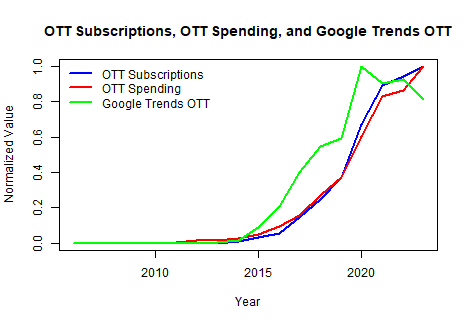
\includegraphics[width=0.8\linewidth]{plots/compare_ott_trends-1}

\subsection{Time Series Decomposition}\label{time-series-decomposition}

\begin{Shaded}
\begin{Highlighting}[]
\CommentTok{\# Extract Cinema Admissions time series}
\NormalTok{cinema\_admissions }\OtherTok{\textless{}{-}}\NormalTok{ ott\_cinema\_monthly.ts[, }\StringTok{"cinema\_admissions"}\NormalTok{]}

\CommentTok{\# a general view of the data}
\FunctionTok{tsdisplay}\NormalTok{(cinema\_admissions, }\AttributeTok{lag.max =} \DecValTok{50}\NormalTok{)}
\end{Highlighting}
\end{Shaded}

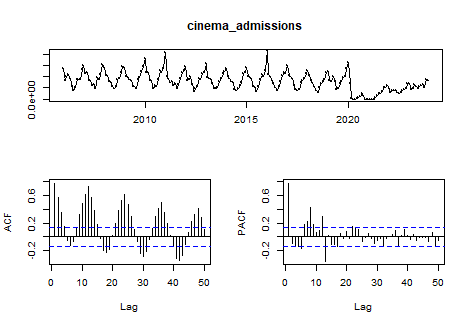
\includegraphics[width=0.8\linewidth]{plots/cinema_admissions-1}

\begin{Shaded}
\begin{Highlighting}[]
\FunctionTok{seasonplot}\NormalTok{(cinema\_admissions, }\AttributeTok{ylab =} \StringTok{"admissions"}\NormalTok{, }\AttributeTok{xlab =} \StringTok{"Year"}\NormalTok{, }\AttributeTok{main =} \StringTok{"Seasonal plot: Cinema Admissions"}\NormalTok{,}
    \AttributeTok{year.labels =}\NormalTok{ T, }\AttributeTok{year.labels.left =}\NormalTok{ T, }\AttributeTok{col =} \DecValTok{1}\SpecialCharTok{:}\DecValTok{20}\NormalTok{, }\AttributeTok{pch =} \DecValTok{19}\NormalTok{)}
\end{Highlighting}
\end{Shaded}

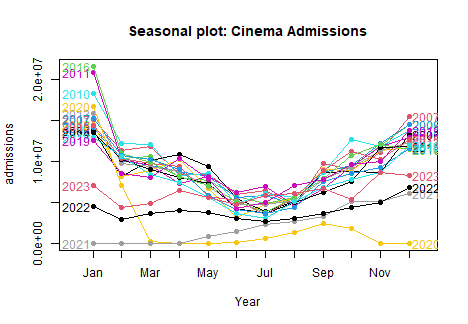
\includegraphics[width=0.8\linewidth]{plots/seasonplot_admissions-1}

\begin{Shaded}
\begin{Highlighting}[]
\CommentTok{\# STL decomposition (Seasonal + Trend + Residual)}
\NormalTok{admissions\_decomposed }\OtherTok{\textless{}{-}} \FunctionTok{stl}\NormalTok{(cinema\_admissions, }\AttributeTok{s.window =} \StringTok{"periodic"}\NormalTok{)}

\CommentTok{\# Plot the decomposed components}
\FunctionTok{plot}\NormalTok{(admissions\_decomposed, }\AttributeTok{main =} \StringTok{"TS Decomposition of Cinema Admissions"}\NormalTok{,}
    \AttributeTok{cex.lab =} \FloatTok{0.45}\NormalTok{, }\AttributeTok{pch =} \DecValTok{16}\NormalTok{, }\AttributeTok{lty =} \DecValTok{1}\NormalTok{, }\AttributeTok{cex =} \FloatTok{0.6}\NormalTok{)}
\end{Highlighting}
\end{Shaded}

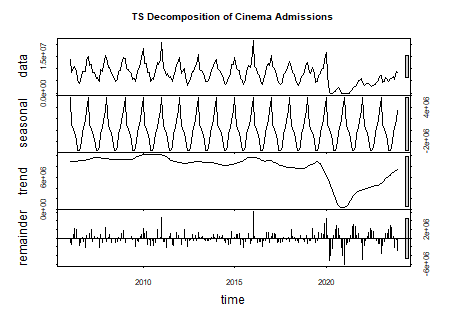
\includegraphics[width=0.8\linewidth]{plots/stl_decomp-1}

\section{2) Time Series Forecasting}\label{time-series-forecasting}

\subsection{Linear Regression}\label{linear-regression}

\begin{Shaded}
\begin{Highlighting}[]
\NormalTok{cinema\_screening }\OtherTok{\textless{}{-}}\NormalTok{ ott\_cinema\_monthly.ts[, }\DecValTok{2}\NormalTok{]}
\NormalTok{cinema\_spending }\OtherTok{\textless{}{-}}\NormalTok{ ott\_cinema\_monthly.ts[, }\DecValTok{3}\NormalTok{]}
\NormalTok{avg\_cinema\_spending\_pp }\OtherTok{\textless{}{-}}\NormalTok{ ott\_cinema\_monthly.ts[, }\DecValTok{4}\NormalTok{]}
\NormalTok{google\_trend\_ott }\OtherTok{\textless{}{-}}\NormalTok{ ott\_cinema\_monthly.ts[, }\DecValTok{5}\NormalTok{]}
\NormalTok{cpi\_all }\OtherTok{\textless{}{-}}\NormalTok{ ott\_cinema\_monthly.ts[, }\DecValTok{6}\NormalTok{]}
\NormalTok{cpi\_culture }\OtherTok{\textless{}{-}}\NormalTok{ ott\_cinema\_monthly.ts[, }\DecValTok{7}\NormalTok{]}
\NormalTok{covid\_cases }\OtherTok{\textless{}{-}}\NormalTok{ ott\_cinema\_monthly.ts[, }\DecValTok{8}\NormalTok{]}

\NormalTok{metrics }\OtherTok{\textless{}{-}} \FunctionTok{c}\NormalTok{(}\StringTok{"Model"}\NormalTok{, }\StringTok{"AIC"}\NormalTok{, }\StringTok{"DW\_Test"}\NormalTok{, }\StringTok{"Ljung\_Box\_pval"}\NormalTok{, }\StringTok{"R2"}\NormalTok{, }\StringTok{"MAE"}\NormalTok{, }\StringTok{"RMSE"}\NormalTok{)}
\NormalTok{model\_performance }\OtherTok{\textless{}{-}} \FunctionTok{data.frame}\NormalTok{(}\FunctionTok{matrix}\NormalTok{(}\AttributeTok{ncol =} \FunctionTok{length}\NormalTok{(metrics), }\AttributeTok{nrow =} \DecValTok{0}\NormalTok{))}
\FunctionTok{colnames}\NormalTok{(model\_performance) }\OtherTok{\textless{}{-}}\NormalTok{ metrics}
\end{Highlighting}
\end{Shaded}

\subsubsection{Multiple Linear Regression with Time
Series}\label{multiple-linear-regression-with-time-series}

\begin{Shaded}
\begin{Highlighting}[]
\CommentTok{\# Fit Initial Full Model}
\NormalTok{full\_tslm }\OtherTok{\textless{}{-}} \FunctionTok{tslm}\NormalTok{(cinema\_admissions }\SpecialCharTok{\textasciitilde{}}\NormalTok{ cinema\_screening }\SpecialCharTok{+}\NormalTok{ cinema\_spending }\SpecialCharTok{+}
\NormalTok{    avg\_cinema\_spending\_pp }\SpecialCharTok{+}\NormalTok{ google\_trend\_ott }\SpecialCharTok{+}\NormalTok{ cpi\_all }\SpecialCharTok{+}\NormalTok{ cpi\_culture }\SpecialCharTok{+}\NormalTok{ covid\_cases }\SpecialCharTok{+}
\NormalTok{    trend }\SpecialCharTok{+}\NormalTok{ season)}
\FunctionTok{summary}\NormalTok{(full\_tslm)}
\end{Highlighting}
\end{Shaded}

\begin{verbatim}

Call:
tslm(formula = cinema_admissions ~ cinema_screening + cinema_spending + 
    avg_cinema_spending_pp + google_trend_ott + cpi_all + cpi_culture + 
    covid_cases + trend + season)

Residuals:
     Min       1Q   Median       3Q      Max 
-1250170  -137734   -29132   143396   975312 

Coefficients:
                         Estimate Std. Error t value Pr(>|t|)    
(Intercept)             6.081e+06  3.522e+05  17.268  < 2e-16 ***
cinema_screening        7.470e-01  5.223e-01   1.430 0.154257    
cinema_spending         1.401e-01  1.782e-03  78.603  < 2e-16 ***
avg_cinema_spending_pp -8.683e+05  5.599e+04 -15.509  < 2e-16 ***
google_trend_ott       -7.570e+02  2.771e+03  -0.273 0.785028    
cpi_all                 1.557e+05  7.050e+04   2.208 0.028387 *  
cpi_culture            -1.115e+04  4.608e+04  -0.242 0.809083    
covid_cases             6.777e-02  5.481e-02   1.236 0.217764    
trend                  -3.161e+03  1.052e+03  -3.005 0.003001 ** 
season2                 3.995e+05  1.163e+05   3.436 0.000721 ***
season3                 4.229e+05  1.195e+05   3.540 0.000501 ***
season4                 2.790e+05  1.215e+05   2.296 0.022731 *  
season5                 3.148e+05  1.334e+05   2.360 0.019281 *  
season6                 2.106e+05  1.470e+05   1.432 0.153695    
season7                 2.040e+05  1.484e+05   1.374 0.170893    
season8                 1.764e+05  1.444e+05   1.222 0.223219    
season9                 3.531e+05  1.330e+05   2.654 0.008603 ** 
season10                3.104e+05  1.186e+05   2.617 0.009554 ** 
season11                6.078e+05  1.157e+05   5.255 3.85e-07 ***
season12                3.296e+05  1.119e+05   2.946 0.003612 ** 
---
Signif. codes:  0 '***' 0.001 '**' 0.01 '*' 0.05 '.' 0.1 ' ' 1

Residual standard error: 281200 on 196 degrees of freedom
Multiple R-squared:  0.9954,    Adjusted R-squared:  0.995 
F-statistic:  2257 on 19 and 196 DF,  p-value: < 2.2e-16
\end{verbatim}

\begin{Shaded}
\begin{Highlighting}[]
\FunctionTok{checkresiduals}\NormalTok{(full\_tslm)}
\end{Highlighting}
\end{Shaded}

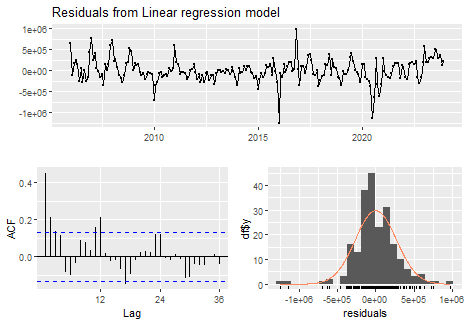
\includegraphics[width=0.8\linewidth]{plots/full_tslm-1}

\begin{verbatim}

    Breusch-Godfrey test for serial correlation of order up to 24

data:  Residuals from Linear regression model
LM test = 68.792, df = 24, p-value = 3.327e-06
\end{verbatim}

\begin{Shaded}
\begin{Highlighting}[]
\NormalTok{model\_name }\OtherTok{\textless{}{-}} \StringTok{"TSLM {-} Full"}
\NormalTok{aic }\OtherTok{\textless{}{-}} \FunctionTok{sprintf}\NormalTok{(}\StringTok{"\%.3f"}\NormalTok{, }\FunctionTok{AIC}\NormalTok{(full\_tslm))}
\NormalTok{dw }\OtherTok{\textless{}{-}} \FunctionTok{sprintf}\NormalTok{(}\StringTok{"\%.3f"}\NormalTok{, }\FunctionTok{as.numeric}\NormalTok{(}\FunctionTok{dwtest}\NormalTok{(full\_tslm)}\SpecialCharTok{$}\NormalTok{statistic))}
\NormalTok{lj\_box }\OtherTok{\textless{}{-}} \ConstantTok{NA}
\NormalTok{r2 }\OtherTok{\textless{}{-}} \FunctionTok{sprintf}\NormalTok{(}\StringTok{"\%.3f"}\NormalTok{, }\FunctionTok{summary}\NormalTok{(full\_tslm)}\SpecialCharTok{$}\NormalTok{r.squared)}
\NormalTok{acc }\OtherTok{\textless{}{-}} \FunctionTok{as.data.frame.array}\NormalTok{(}\FunctionTok{accuracy}\NormalTok{(full\_tslm))}
\NormalTok{mae }\OtherTok{\textless{}{-}} \FunctionTok{format}\NormalTok{(acc}\SpecialCharTok{$}\NormalTok{MAE, }\AttributeTok{big.mark =} \StringTok{","}\NormalTok{, }\AttributeTok{nsmall =} \DecValTok{2}\NormalTok{, }\AttributeTok{scientific =} \ConstantTok{FALSE}\NormalTok{)}
\NormalTok{rmse }\OtherTok{\textless{}{-}} \FunctionTok{format}\NormalTok{(acc}\SpecialCharTok{$}\NormalTok{RMSE, }\AttributeTok{big.mark =} \StringTok{","}\NormalTok{, }\AttributeTok{nsmall =} \DecValTok{2}\NormalTok{, }\AttributeTok{scientific =} \ConstantTok{FALSE}\NormalTok{)}



\NormalTok{model\_performance[}\FunctionTok{nrow}\NormalTok{(model\_performance) }\SpecialCharTok{+} \DecValTok{1}\NormalTok{, ] }\OtherTok{\textless{}{-}} \FunctionTok{c}\NormalTok{(model\_name, aic, dw,}
\NormalTok{    lj\_box, r2, mae, rmse)}
\end{Highlighting}
\end{Shaded}

\subsubsection{Stepwise Regression}\label{stepwise-regression}

\begin{Shaded}
\begin{Highlighting}[]
\CommentTok{\# Convert tslm object to lm object}
\NormalTok{full\_lm }\OtherTok{\textless{}{-}} \FunctionTok{lm}\NormalTok{(}\FunctionTok{formula}\NormalTok{(full\_tslm), }\AttributeTok{data =} \FunctionTok{as.data.frame}\NormalTok{(ott\_cinema\_monthly.ts))}

\CommentTok{\# Stepwise Selection (Both Directions: Forward \& Backward)}
\NormalTok{stepwise\_model }\OtherTok{\textless{}{-}} \FunctionTok{step}\NormalTok{(full\_lm, }\AttributeTok{direction =} \StringTok{"both"}\NormalTok{, }\AttributeTok{trace =} \ConstantTok{TRUE}\NormalTok{)}
\end{Highlighting}
\end{Shaded}

\begin{verbatim}
Start:  AIC=5439.29
cinema_admissions ~ cinema_screening + cinema_spending + avg_cinema_spending_pp + 
    google_trend_ott + cpi_all + cpi_culture + covid_cases + 
    trend + season

                         Df  Sum of Sq        RSS    AIC
- cpi_culture             1 4.6294e+09 1.5506e+13 5437.4
- google_trend_ott        1 5.9009e+09 1.5508e+13 5437.4
- covid_cases             1 1.2092e+11 1.5623e+13 5439.0
<none>                                 1.5502e+13 5439.3
- cinema_screening        1 1.6177e+11 1.5664e+13 5439.5
- cpi_all                 1 3.8567e+11 1.5888e+13 5442.6
- trend                   1 7.1430e+11 1.6216e+13 5447.0
- season                 11 3.5230e+12 1.9025e+13 5461.5
- avg_cinema_spending_pp  1 1.9024e+13 3.4525e+13 5610.2
- cinema_spending         1 4.8865e+14 5.0415e+14 6189.4

Step:  AIC=5437.35
cinema_admissions ~ cinema_screening + cinema_spending + avg_cinema_spending_pp + 
    google_trend_ott + cpi_all + covid_cases + trend + season

                         Df  Sum of Sq        RSS    AIC
- google_trend_ott        1 7.0217e+09 1.5513e+13 5435.4
- covid_cases             1 1.2145e+11 1.5628e+13 5437.0
<none>                                 1.5506e+13 5437.4
- cinema_screening        1 1.6011e+11 1.5667e+13 5437.6
+ cpi_culture             1 4.6294e+09 1.5502e+13 5439.3
- cpi_all                 1 3.8115e+11 1.5888e+13 5440.6
- trend                   1 7.1058e+11 1.6217e+13 5445.0
- season                 11 3.5906e+12 1.9097e+13 5460.3
- avg_cinema_spending_pp  1 1.9144e+13 3.4651e+13 5609.0
- cinema_spending         1 4.9224e+14 5.0775e+14 6188.9

Step:  AIC=5435.45
cinema_admissions ~ cinema_screening + cinema_spending + avg_cinema_spending_pp + 
    cpi_all + covid_cases + trend + season

                         Df  Sum of Sq        RSS    AIC
- covid_cases             1 1.1562e+11 1.5629e+13 5435.1
<none>                                 1.5513e+13 5435.4
+ google_trend_ott        1 7.0217e+09 1.5506e+13 5437.4
+ cpi_culture             1 5.7502e+09 1.5508e+13 5437.4
- cinema_screening        1 3.3315e+11 1.5847e+13 5438.0
- cpi_all                 1 3.7529e+11 1.5889e+13 5438.6
- season                 11 3.6136e+12 1.9127e+13 5458.7
- trend                   1 3.3740e+12 1.8888e+13 5476.0
- avg_cinema_spending_pp  1 1.9306e+13 3.4819e+13 5608.1
- cinema_spending         1 4.9279e+14 5.0830e+14 6187.2

Step:  AIC=5435.05
cinema_admissions ~ cinema_screening + cinema_spending + avg_cinema_spending_pp + 
    cpi_all + trend + season

                         Df  Sum of Sq        RSS    AIC
<none>                                 1.5629e+13 5435.1
+ covid_cases             1 1.1562e+11 1.5513e+13 5435.4
+ cpi_culture             1 5.5972e+09 1.5624e+13 5437.0
+ google_trend_ott        1 1.1910e+09 1.5628e+13 5437.0
- cinema_screening        1 3.5284e+11 1.5982e+13 5437.9
- cpi_all                 1 7.0313e+11 1.6332e+13 5442.6
- season                 11 3.6449e+12 1.9274e+13 5458.3
- trend                   1 3.2813e+12 1.8910e+13 5474.2
- avg_cinema_spending_pp  1 1.9229e+13 3.4858e+13 5606.3
- cinema_spending         1 5.2254e+14 5.3817e+14 6197.5
\end{verbatim}

\begin{Shaded}
\begin{Highlighting}[]
\CommentTok{\# Display Summary of Selected Model}
\FunctionTok{summary}\NormalTok{(stepwise\_model)}
\end{Highlighting}
\end{Shaded}

\begin{verbatim}

Call:
lm(formula = cinema_admissions ~ cinema_screening + cinema_spending + 
    avg_cinema_spending_pp + cpi_all + trend + season, data = as.data.frame(ott_cinema_monthly.ts))

Residuals:
     Min       1Q   Median       3Q      Max 
-1227239  -135008   -25772   146570   969888 

Coefficients:
                         Estimate Std. Error t value Pr(>|t|)    
(Intercept)             6.119e+06  3.489e+05  17.539  < 2e-16 ***
cinema_screening        8.629e-01  4.071e-01   2.120 0.035281 *  
cinema_spending         1.396e-01  1.711e-03  81.568  < 2e-16 ***
avg_cinema_spending_pp -8.683e+05  5.549e+04 -15.647  < 2e-16 ***
cpi_all                 1.879e+05  6.280e+04   2.992 0.003121 ** 
trend                  -3.336e+03  5.162e+02  -6.464 7.71e-10 ***
season2                 3.720e+05  1.093e+05   3.402 0.000808 ***
season3                 3.953e+05  1.146e+05   3.448 0.000689 ***
season4                 2.518e+05  1.161e+05   2.169 0.031258 *  
season5                 2.868e+05  1.234e+05   2.324 0.021133 *  
season6                 1.702e+05  1.336e+05   1.274 0.204004    
season7                 1.695e+05  1.306e+05   1.298 0.195835    
season8                 1.319e+05  1.248e+05   1.057 0.291772    
season9                 3.430e+05  1.229e+05   2.790 0.005777 ** 
season10                2.784e+05  1.121e+05   2.483 0.013871 *  
season11                5.909e+05  1.126e+05   5.248 3.93e-07 ***
season12                2.984e+05  9.822e+04   3.038 0.002698 ** 
---
Signif. codes:  0 '***' 0.001 '**' 0.01 '*' 0.05 '.' 0.1 ' ' 1

Residual standard error: 280200 on 199 degrees of freedom
Multiple R-squared:  0.9954,    Adjusted R-squared:  0.995 
F-statistic:  2699 on 16 and 199 DF,  p-value: < 2.2e-16
\end{verbatim}

\begin{Shaded}
\begin{Highlighting}[]
\FunctionTok{checkresiduals}\NormalTok{(stepwise\_model)}
\end{Highlighting}
\end{Shaded}

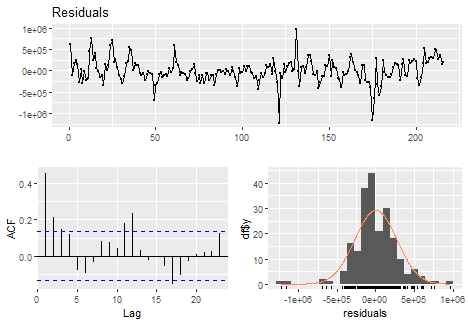
\includegraphics[width=0.8\linewidth]{plots/stepwise_tslm-1}

\begin{verbatim}

    Breusch-Godfrey test for serial correlation of order up to 20

data:  Residuals
LM test = 68.12, df = 20, p-value = 3.682e-07
\end{verbatim}

\begin{Shaded}
\begin{Highlighting}[]
\FunctionTok{dwtest}\NormalTok{(stepwise\_model)  }\CommentTok{\#indicates a problem of positive autocorrelation}
\end{Highlighting}
\end{Shaded}

\begin{verbatim}

    Durbin-Watson test

data:  stepwise_model
DW = 1.0635, p-value = 2.92e-12
alternative hypothesis: true autocorrelation is greater than 0
\end{verbatim}

\begin{Shaded}
\begin{Highlighting}[]
\NormalTok{model\_name }\OtherTok{\textless{}{-}} \StringTok{"TSLM {-} Stepwise"}
\NormalTok{aic }\OtherTok{\textless{}{-}} \FunctionTok{sprintf}\NormalTok{(}\StringTok{"\%.3f"}\NormalTok{, }\FunctionTok{AIC}\NormalTok{(stepwise\_model))}
\NormalTok{dw }\OtherTok{\textless{}{-}} \FunctionTok{sprintf}\NormalTok{(}\StringTok{"\%.3f"}\NormalTok{, }\FunctionTok{as.numeric}\NormalTok{(}\FunctionTok{dwtest}\NormalTok{(stepwise\_model)}\SpecialCharTok{$}\NormalTok{statistic))}
\NormalTok{lj\_box }\OtherTok{\textless{}{-}} \ConstantTok{NA}
\NormalTok{r2 }\OtherTok{\textless{}{-}} \FunctionTok{sprintf}\NormalTok{(}\StringTok{"\%.3f"}\NormalTok{, }\FunctionTok{summary}\NormalTok{(stepwise\_model)}\SpecialCharTok{$}\NormalTok{r.squared)}
\NormalTok{acc }\OtherTok{\textless{}{-}} \FunctionTok{as.data.frame.array}\NormalTok{(}\FunctionTok{accuracy}\NormalTok{(stepwise\_model))}
\NormalTok{mae }\OtherTok{\textless{}{-}} \FunctionTok{format}\NormalTok{(acc}\SpecialCharTok{$}\NormalTok{MAE, }\AttributeTok{big.mark =} \StringTok{","}\NormalTok{, }\AttributeTok{nsmall =} \DecValTok{2}\NormalTok{, }\AttributeTok{scientific =} \ConstantTok{FALSE}\NormalTok{)}
\NormalTok{rmse }\OtherTok{\textless{}{-}} \FunctionTok{format}\NormalTok{(acc}\SpecialCharTok{$}\NormalTok{RMSE, }\AttributeTok{big.mark =} \StringTok{","}\NormalTok{, }\AttributeTok{nsmall =} \DecValTok{2}\NormalTok{, }\AttributeTok{scientific =} \ConstantTok{FALSE}\NormalTok{)}

\NormalTok{model\_performance[}\FunctionTok{nrow}\NormalTok{(model\_performance) }\SpecialCharTok{+} \DecValTok{1}\NormalTok{, ] }\OtherTok{\textless{}{-}} \FunctionTok{c}\NormalTok{(model\_name, aic, dw,}
\NormalTok{    lj\_box, r2, mae, rmse)}
\end{Highlighting}
\end{Shaded}

\begin{Shaded}
\begin{Highlighting}[]
\CommentTok{\# Extract fitted values from stepwise model}
\NormalTok{fitted\_stepwise }\OtherTok{\textless{}{-}} \FunctionTok{fitted}\NormalTok{(stepwise\_model)}

\CommentTok{\# Convert fitted values into a time series object}
\NormalTok{fitted\_stepwise.ts }\OtherTok{\textless{}{-}} \FunctionTok{ts}\NormalTok{(fitted\_stepwise, }\AttributeTok{start =} \FunctionTok{start}\NormalTok{(cinema\_admissions),}
    \AttributeTok{frequency =} \FunctionTok{frequency}\NormalTok{(cinema\_admissions))}


\FunctionTok{plot}\NormalTok{(cinema\_admissions, }\AttributeTok{type =} \StringTok{"o"}\NormalTok{, }\AttributeTok{pch =} \DecValTok{16}\NormalTok{, }\AttributeTok{cex =} \FloatTok{0.6}\NormalTok{, }\AttributeTok{main =} \StringTok{"Actual vs. Stepwise Model Predictions"}\NormalTok{)}

\CommentTok{\# Add Stepwise Regression Predictions}
\FunctionTok{lines}\NormalTok{(fitted\_stepwise.ts, }\AttributeTok{col =} \StringTok{"orange2"}\NormalTok{, }\AttributeTok{lwd =} \DecValTok{2}\NormalTok{, }\AttributeTok{lty =} \DecValTok{1}\NormalTok{)}

\CommentTok{\# Add Legend}
\FunctionTok{legend}\NormalTok{(}\StringTok{"topright"}\NormalTok{, }\AttributeTok{legend =} \FunctionTok{c}\NormalTok{(}\StringTok{"Observed"}\NormalTok{, }\StringTok{"Predicted (Stepwise)"}\NormalTok{), }\AttributeTok{col =} \FunctionTok{c}\NormalTok{(}\StringTok{"black"}\NormalTok{,}
    \StringTok{"orange2"}\NormalTok{), }\AttributeTok{lwd =} \FunctionTok{c}\NormalTok{(}\DecValTok{1}\NormalTok{, }\DecValTok{2}\NormalTok{), }\AttributeTok{lty =} \FunctionTok{c}\NormalTok{(}\DecValTok{1}\NormalTok{, }\DecValTok{1}\NormalTok{), }\AttributeTok{bty =} \StringTok{"n"}\NormalTok{)}
\end{Highlighting}
\end{Shaded}

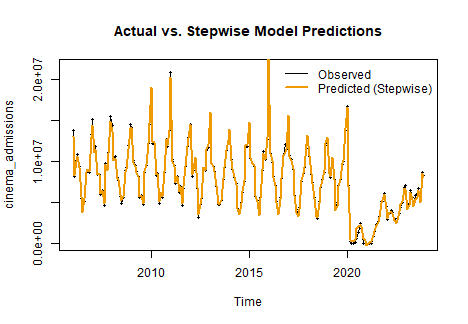
\includegraphics[width=0.8\linewidth]{plots/stepwise_regression-1}

\subsection{ARIMA Models}\label{arima-models}

General indication (for differenced data): - If the ACF is exponentially
decaying or sinusoidal and there is a significant spike at lag p in PACF
and nothing else, it may be an ARIMA(p,d,0). - If the PACF is
exponentially decaying or sinusoidal and there is a significant spike at
lag q in ACF and nothing else, it may be an ARIMA(0,d,q).

\begin{Shaded}
\begin{Highlighting}[]
\NormalTok{diff1 }\OtherTok{\textless{}{-}} \FunctionTok{diff}\NormalTok{(cinema\_admissions)}
\FunctionTok{tsdisplay}\NormalTok{(diff1, }\AttributeTok{main =} \StringTok{"cinema\_admissions (d=1)"}\NormalTok{)}
\end{Highlighting}
\end{Shaded}

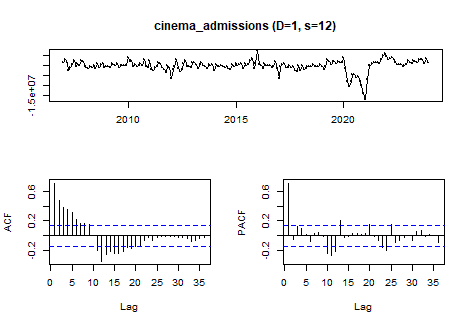
\includegraphics[width=0.8\linewidth]{plots/diff_d1-1}

\begin{Shaded}
\begin{Highlighting}[]
\NormalTok{diff2 }\OtherTok{\textless{}{-}} \FunctionTok{diff}\NormalTok{(cinema\_admissions, }\AttributeTok{lag =} \DecValTok{12}\NormalTok{)}
\FunctionTok{tsdisplay}\NormalTok{(diff2, }\AttributeTok{main =} \StringTok{"cinema\_admissions (D=1, s=12)"}\NormalTok{)}
\end{Highlighting}
\end{Shaded}

\includegraphics[width=0.8\linewidth]{plots/diff_D1-1}

\begin{Shaded}
\begin{Highlighting}[]
\NormalTok{diff3 }\OtherTok{\textless{}{-}} \FunctionTok{diff}\NormalTok{(diff1, }\AttributeTok{lag =} \DecValTok{12}\NormalTok{)}
\FunctionTok{tsdisplay}\NormalTok{(diff3, }\AttributeTok{main =} \StringTok{"cinema\_admissions (d=1, D=1, s=12)"}\NormalTok{)}
\end{Highlighting}
\end{Shaded}

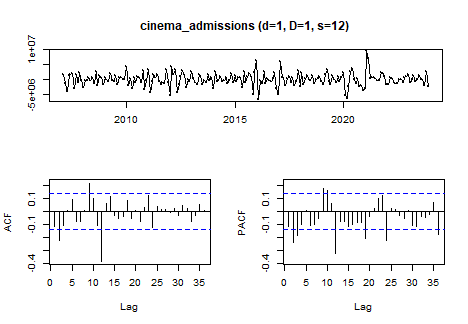
\includegraphics[width=0.8\linewidth]{plots/diff_d1_D1-1}

\subsubsection{ARIMA}\label{arima}

\begin{Shaded}
\begin{Highlighting}[]
\CommentTok{\# first Arima model}
\NormalTok{arima1.cinema\_admissions }\OtherTok{\textless{}{-}} \FunctionTok{Arima}\NormalTok{(cinema\_admissions, }\AttributeTok{order =} \FunctionTok{c}\NormalTok{(}\DecValTok{2}\NormalTok{, }\DecValTok{1}\NormalTok{, }\DecValTok{2}\NormalTok{),}
    \AttributeTok{seasonal =} \FunctionTok{c}\NormalTok{(}\DecValTok{1}\NormalTok{, }\DecValTok{1}\NormalTok{, }\DecValTok{1}\NormalTok{))}
\FunctionTok{summary}\NormalTok{(arima1.cinema\_admissions)}
\end{Highlighting}
\end{Shaded}

\begin{verbatim}
Series: cinema_admissions 
ARIMA(2,1,2)(1,1,1)[12] 

Coefficients:
\end{verbatim}

\begin{verbatim}
          ar1     ar2      ma1      ma2    sar1     sma1
      -0.1567  0.5244  -0.1131  -0.7413  0.1432  -0.8180
s.e.      NaN     NaN      NaN      NaN  0.1264   0.1034

sigma^2 = 2.966e+12:  log likelihood = -3205.77
AIC=6425.54   AICc=6426.12   BIC=6448.73

Training set error measures:
                    ME    RMSE     MAE MPE MAPE      MASE         ACF1
Training set -45240.41 1644855 1174837 NaN  Inf 0.6610072 -0.008085536
\end{verbatim}

\begin{Shaded}
\begin{Highlighting}[]
\NormalTok{fit.arima1.cinema\_admissions }\OtherTok{\textless{}{-}} \FunctionTok{fitted}\NormalTok{(arima1.cinema\_admissions)}

\FunctionTok{plot}\NormalTok{(cinema\_admissions, }\AttributeTok{type =} \StringTok{"o"}\NormalTok{, }\AttributeTok{pch =} \DecValTok{16}\NormalTok{, }\AttributeTok{cex =} \FloatTok{0.6}\NormalTok{, }\AttributeTok{ylab =} \StringTok{"Admissions"}\NormalTok{,}
    \AttributeTok{main =} \StringTok{"Observed vs. ARIMA(2,1,2)(1,1,1)[12] predictions"}\NormalTok{)}
\FunctionTok{lines}\NormalTok{(fit.arima1.cinema\_admissions, }\AttributeTok{col =} \StringTok{"orange2"}\NormalTok{, }\AttributeTok{lwd =} \DecValTok{2}\NormalTok{)}
\FunctionTok{legend}\NormalTok{(}\StringTok{"topright"}\NormalTok{, }\AttributeTok{legend =} \FunctionTok{c}\NormalTok{(}\StringTok{"Observed"}\NormalTok{, }\StringTok{"ARIMA"}\NormalTok{), }\AttributeTok{col =} \FunctionTok{c}\NormalTok{(}\StringTok{"black"}\NormalTok{, }\StringTok{"orange2"}\NormalTok{),}
    \AttributeTok{lwd =} \FunctionTok{c}\NormalTok{(}\DecValTok{1}\NormalTok{, }\DecValTok{2}\NormalTok{), }\AttributeTok{lty =} \FunctionTok{c}\NormalTok{(}\DecValTok{1}\NormalTok{, }\DecValTok{1}\NormalTok{), }\AttributeTok{bty =} \StringTok{"n"}\NormalTok{)}
\end{Highlighting}
\end{Shaded}

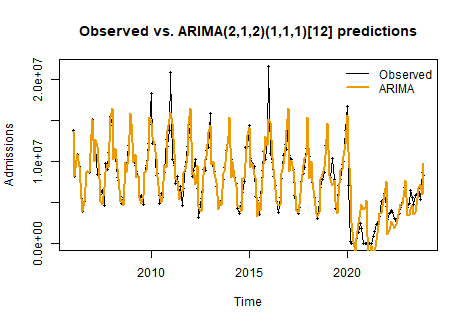
\includegraphics[width=0.8\linewidth]{plots/arima1-1}

\begin{Shaded}
\begin{Highlighting}[]
\NormalTok{res.arima1.cinema\_admissions }\OtherTok{\textless{}{-}} \FunctionTok{residuals}\NormalTok{(arima1.cinema\_admissions)}
\FunctionTok{tsdisplay}\NormalTok{(res.arima1.cinema\_admissions)}
\end{Highlighting}
\end{Shaded}

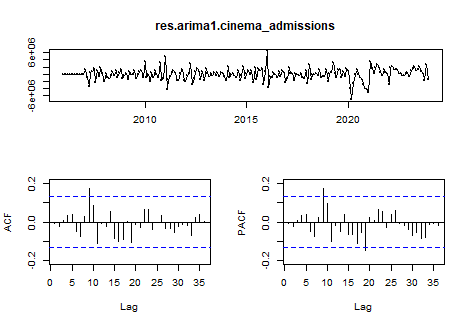
\includegraphics[width=0.8\linewidth]{plots/arima1-2}

\begin{Shaded}
\begin{Highlighting}[]
\FunctionTok{checkresiduals}\NormalTok{(arima1.cinema\_admissions)}
\end{Highlighting}
\end{Shaded}

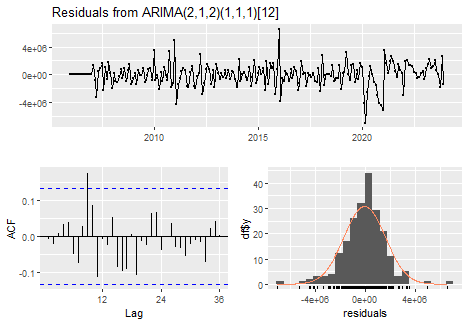
\includegraphics[width=0.8\linewidth]{plots/arima1-3}

\begin{verbatim}

    Ljung-Box test

data:  Residuals from ARIMA(2,1,2)(1,1,1)[12]
Q* = 27.082, df = 18, p-value = 0.07747

Model df: 6.   Total lags used: 24
\end{verbatim}

\begin{Shaded}
\begin{Highlighting}[]
\NormalTok{model\_name }\OtherTok{\textless{}{-}} \StringTok{"ARIMA(2,1,2)(1,1,1)12"}
\NormalTok{aic }\OtherTok{\textless{}{-}} \FunctionTok{sprintf}\NormalTok{(}\StringTok{"\%.3f"}\NormalTok{, }\FunctionTok{AIC}\NormalTok{(arima1.cinema\_admissions))}
\NormalTok{dw }\OtherTok{\textless{}{-}} \ConstantTok{NA}
\NormalTok{lj\_box }\OtherTok{\textless{}{-}} \FunctionTok{sprintf}\NormalTok{(}\StringTok{"\%.3f"}\NormalTok{, }\FunctionTok{checkresiduals}\NormalTok{(arima1.cinema\_admissions)}\SpecialCharTok{$}\NormalTok{p.value)}
\end{Highlighting}
\end{Shaded}

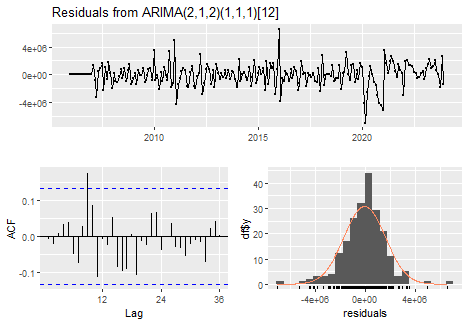
\includegraphics[width=0.8\linewidth]{plots/arima1_metrics-1}

\begin{verbatim}

    Ljung-Box test

data:  Residuals from ARIMA(2,1,2)(1,1,1)[12]
Q* = 27.082, df = 18, p-value = 0.07747

Model df: 6.   Total lags used: 24
\end{verbatim}

\begin{Shaded}
\begin{Highlighting}[]
\NormalTok{r2 }\OtherTok{\textless{}{-}} \FunctionTok{sprintf}\NormalTok{(}\StringTok{"\%.3f"}\NormalTok{, }\FunctionTok{R2\_Score}\NormalTok{(fit.arima1.cinema\_admissions, cinema\_admissions))}
\NormalTok{acc }\OtherTok{\textless{}{-}} \FunctionTok{as.data.frame.array}\NormalTok{(}\FunctionTok{accuracy}\NormalTok{(arima1.cinema\_admissions))}
\NormalTok{mae }\OtherTok{\textless{}{-}} \FunctionTok{format}\NormalTok{(acc}\SpecialCharTok{$}\NormalTok{MAE, }\AttributeTok{big.mark =} \StringTok{","}\NormalTok{, }\AttributeTok{nsmall =} \DecValTok{2}\NormalTok{, }\AttributeTok{scientific =} \ConstantTok{FALSE}\NormalTok{)}
\NormalTok{rmse }\OtherTok{\textless{}{-}} \FunctionTok{format}\NormalTok{(acc}\SpecialCharTok{$}\NormalTok{RMSE, }\AttributeTok{big.mark =} \StringTok{","}\NormalTok{, }\AttributeTok{nsmall =} \DecValTok{2}\NormalTok{, }\AttributeTok{scientific =} \ConstantTok{FALSE}\NormalTok{)}

\NormalTok{model\_performance[}\FunctionTok{nrow}\NormalTok{(model\_performance) }\SpecialCharTok{+} \DecValTok{1}\NormalTok{, ] }\OtherTok{\textless{}{-}} \FunctionTok{c}\NormalTok{(model\_name, aic, dw,}
\NormalTok{    lj\_box, r2, mae, rmse)}
\end{Highlighting}
\end{Shaded}

\begin{Shaded}
\begin{Highlighting}[]
\NormalTok{arima.a.cinema\_admissions }\OtherTok{\textless{}{-}} \FunctionTok{auto.arima}\NormalTok{(cinema\_admissions)}
\FunctionTok{summary}\NormalTok{(arima.a.cinema\_admissions)}
\end{Highlighting}
\end{Shaded}

\begin{verbatim}
Series: cinema_admissions 
ARIMA(1,0,2)(0,1,1)[12] 

Coefficients:
         ar1      ma1      ma2     sma1
      0.8946  -0.2130  -0.1664  -0.6699
s.e.  0.0531   0.0939   0.0920   0.0668

sigma^2 = 2.931e+12:  log likelihood = -3219.36
AIC=6448.71   AICc=6449.01   BIC=6465.3

Training set error measures:
                    ME    RMSE     MAE MPE MAPE      MASE        ACF1
Training set -98286.64 1647445 1158030 NaN  Inf 0.6515513 0.007339816
\end{verbatim}

\begin{Shaded}
\begin{Highlighting}[]
\NormalTok{fit.arima.a.cinema\_admissions }\OtherTok{\textless{}{-}} \FunctionTok{fitted}\NormalTok{(arima.a.cinema\_admissions)}

\FunctionTok{plot}\NormalTok{(cinema\_admissions, }\AttributeTok{type =} \StringTok{"o"}\NormalTok{, }\AttributeTok{pch =} \DecValTok{16}\NormalTok{, }\AttributeTok{cex =} \FloatTok{0.6}\NormalTok{, }\AttributeTok{ylab =} \StringTok{"Admissions"}\NormalTok{,}
    \AttributeTok{main =} \StringTok{"Observed vs. autoARIMA predictions"}\NormalTok{)}
\FunctionTok{lines}\NormalTok{(fit.arima.a.cinema\_admissions, }\AttributeTok{col =} \StringTok{"purple2"}\NormalTok{, }\AttributeTok{lwd =} \DecValTok{2}\NormalTok{)}
\FunctionTok{legend}\NormalTok{(}\StringTok{"topright"}\NormalTok{, }\AttributeTok{legend =} \FunctionTok{c}\NormalTok{(}\StringTok{"Observed"}\NormalTok{, }\StringTok{"autoARIMA"}\NormalTok{), }\AttributeTok{col =} \FunctionTok{c}\NormalTok{(}\StringTok{"black"}\NormalTok{,}
    \StringTok{"purple2"}\NormalTok{), }\AttributeTok{lwd =} \FunctionTok{c}\NormalTok{(}\DecValTok{1}\NormalTok{, }\DecValTok{2}\NormalTok{), }\AttributeTok{lty =} \FunctionTok{c}\NormalTok{(}\DecValTok{1}\NormalTok{, }\DecValTok{1}\NormalTok{), }\AttributeTok{bty =} \StringTok{"n"}\NormalTok{)}
\end{Highlighting}
\end{Shaded}

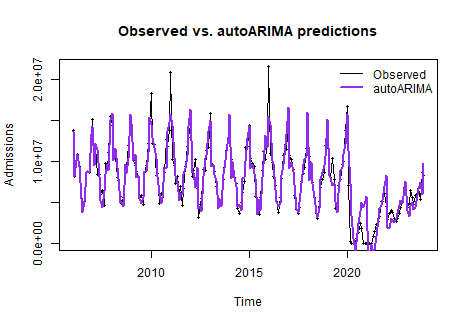
\includegraphics[width=0.8\linewidth]{plots/auto_arima-1}

\begin{Shaded}
\begin{Highlighting}[]
\NormalTok{res.arima.a.cinema\_admissions }\OtherTok{\textless{}{-}} \FunctionTok{residuals}\NormalTok{(arima.a.cinema\_admissions)}
\FunctionTok{tsdisplay}\NormalTok{(res.arima.a.cinema\_admissions)}
\end{Highlighting}
\end{Shaded}

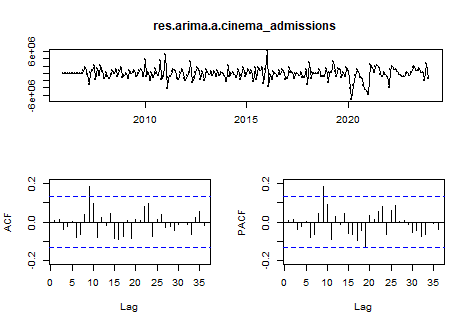
\includegraphics[width=0.8\linewidth]{plots/auto_arima-2}

\begin{Shaded}
\begin{Highlighting}[]
\FunctionTok{checkresiduals}\NormalTok{(arima.a.cinema\_admissions)}
\end{Highlighting}
\end{Shaded}

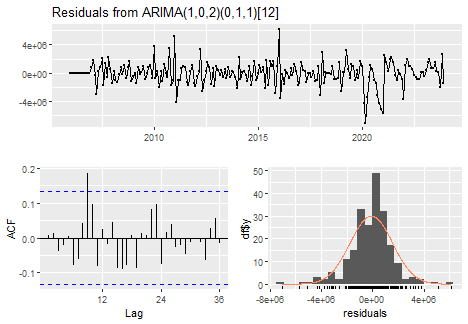
\includegraphics[width=0.8\linewidth]{plots/auto_arima-3}

\begin{verbatim}

    Ljung-Box test

data:  Residuals from ARIMA(1,0,2)(0,1,1)[12]
Q* = 28.071, df = 20, p-value = 0.1077

Model df: 4.   Total lags used: 24
\end{verbatim}

\begin{Shaded}
\begin{Highlighting}[]
\NormalTok{model\_name }\OtherTok{\textless{}{-}} \StringTok{"auto.ARIMA"}
\NormalTok{aic }\OtherTok{\textless{}{-}} \FunctionTok{sprintf}\NormalTok{(}\StringTok{"\%.3f"}\NormalTok{, }\FunctionTok{AIC}\NormalTok{(arima.a.cinema\_admissions))}
\NormalTok{dw }\OtherTok{\textless{}{-}} \ConstantTok{NA}
\NormalTok{lj\_box }\OtherTok{\textless{}{-}} \FunctionTok{sprintf}\NormalTok{(}\StringTok{"\%.3f"}\NormalTok{, }\FunctionTok{checkresiduals}\NormalTok{(arima.a.cinema\_admissions)}\SpecialCharTok{$}\NormalTok{p.value)}
\end{Highlighting}
\end{Shaded}

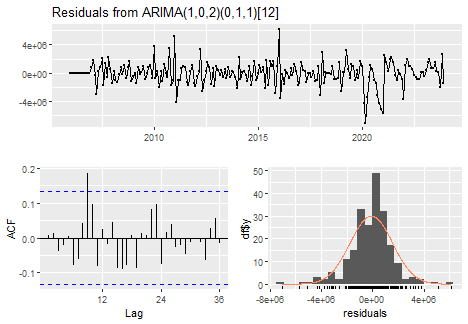
\includegraphics[width=0.8\linewidth]{plots/auto_arima_metrics-1}

\begin{verbatim}

    Ljung-Box test

data:  Residuals from ARIMA(1,0,2)(0,1,1)[12]
Q* = 28.071, df = 20, p-value = 0.1077

Model df: 4.   Total lags used: 24
\end{verbatim}

\begin{Shaded}
\begin{Highlighting}[]
\NormalTok{r2 }\OtherTok{\textless{}{-}} \FunctionTok{sprintf}\NormalTok{(}\StringTok{"\%.3f"}\NormalTok{, }\FunctionTok{R2\_Score}\NormalTok{(fit.arima.a.cinema\_admissions, cinema\_admissions))}
\NormalTok{acc }\OtherTok{\textless{}{-}} \FunctionTok{as.data.frame.array}\NormalTok{(}\FunctionTok{accuracy}\NormalTok{(arima.a.cinema\_admissions))}
\NormalTok{mae }\OtherTok{\textless{}{-}} \FunctionTok{format}\NormalTok{(acc}\SpecialCharTok{$}\NormalTok{MAE, }\AttributeTok{big.mark =} \StringTok{","}\NormalTok{, }\AttributeTok{nsmall =} \DecValTok{2}\NormalTok{, }\AttributeTok{scientific =} \ConstantTok{FALSE}\NormalTok{)}
\NormalTok{rmse }\OtherTok{\textless{}{-}} \FunctionTok{format}\NormalTok{(acc}\SpecialCharTok{$}\NormalTok{RMSE, }\AttributeTok{big.mark =} \StringTok{","}\NormalTok{, }\AttributeTok{nsmall =} \DecValTok{2}\NormalTok{, }\AttributeTok{scientific =} \ConstantTok{FALSE}\NormalTok{)}

\NormalTok{model\_performance[}\FunctionTok{nrow}\NormalTok{(model\_performance) }\SpecialCharTok{+} \DecValTok{1}\NormalTok{, ] }\OtherTok{\textless{}{-}} \FunctionTok{c}\NormalTok{(model\_name, aic, dw,}
\NormalTok{    lj\_box, r2, mae, rmse)}
\end{Highlighting}
\end{Shaded}

\subsubsection{ARIMAx}\label{arimax}

\begin{Shaded}
\begin{Highlighting}[]
\NormalTok{xreg1 }\OtherTok{\textless{}{-}} \FunctionTok{cbind}\NormalTok{(cinema\_screening, cinema\_spending, avg\_cinema\_spending\_pp,}
\NormalTok{    cpi\_all)}

\NormalTok{sarimax\_model1 }\OtherTok{\textless{}{-}} \FunctionTok{auto.arima}\NormalTok{(cinema\_admissions, }\AttributeTok{xreg =}\NormalTok{ xreg1)}
\FunctionTok{summary}\NormalTok{(sarimax\_model1)}
\end{Highlighting}
\end{Shaded}

\begin{verbatim}
Series: cinema_admissions 
Regression with ARIMA(3,1,0)(2,0,1)[12] errors 

Coefficients:
          ar1      ar2      ar3    sar1    sar2     sma1  cinema_screening
      -0.4251  -0.3035  -0.1890  0.7920  0.0096  -0.4090            2.2637
s.e.   0.0674   0.0712   0.0685  0.2474  0.1549   0.2413            0.6136
      cinema_spending  avg_cinema_spending_pp   cpi_all
               0.1358              -837865.17  43073.56
s.e.           0.0016                45654.96  51621.39

sigma^2 = 6.334e+10:  log likelihood = -2976.33
AIC=5974.66   AICc=5975.96   BIC=6011.73

Training set error measures:
                    ME     RMSE      MAE MPE MAPE       MASE         ACF1
Training set -3309.766 245186.5 170544.1 NaN  Inf 0.09595449 -0.008151537
\end{verbatim}

\begin{Shaded}
\begin{Highlighting}[]
\NormalTok{fit.sarimax1 }\OtherTok{\textless{}{-}} \FunctionTok{fitted}\NormalTok{(sarimax\_model1)}

\FunctionTok{plot}\NormalTok{(cinema\_admissions, }\AttributeTok{type =} \StringTok{"o"}\NormalTok{, }\AttributeTok{pch =} \DecValTok{16}\NormalTok{, }\AttributeTok{cex =} \FloatTok{0.6}\NormalTok{)}
\FunctionTok{lines}\NormalTok{(fit.sarimax1, }\AttributeTok{col =} \StringTok{"purple2"}\NormalTok{, }\AttributeTok{lwd =} \DecValTok{2}\NormalTok{)}
\end{Highlighting}
\end{Shaded}

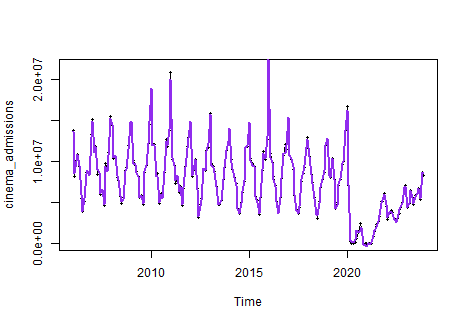
\includegraphics[width=0.8\linewidth]{plots/auto_sarimax1-1}

\begin{Shaded}
\begin{Highlighting}[]
\NormalTok{res.sarimax\_model1 }\OtherTok{\textless{}{-}} \FunctionTok{residuals}\NormalTok{(sarimax\_model1)}
\FunctionTok{tsdisplay}\NormalTok{(res.sarimax\_model1)}
\end{Highlighting}
\end{Shaded}

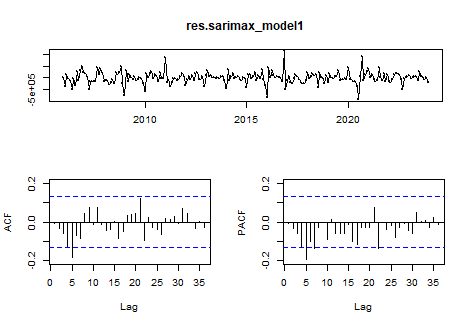
\includegraphics[width=0.8\linewidth]{plots/auto_sarimax1-2}

\begin{Shaded}
\begin{Highlighting}[]
\FunctionTok{checkresiduals}\NormalTok{(sarimax\_model1)}
\end{Highlighting}
\end{Shaded}

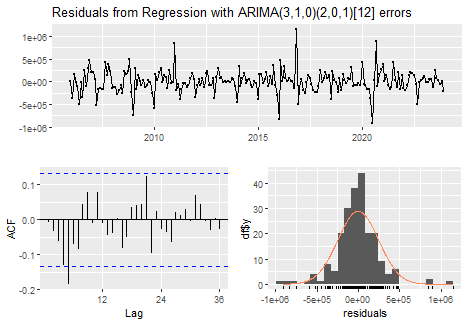
\includegraphics[width=0.8\linewidth]{plots/auto_sarimax1-3}

\begin{verbatim}

    Ljung-Box test

data:  Residuals from Regression with ARIMA(3,1,0)(2,0,1)[12] errors
Q* = 29.078, df = 18, p-value = 0.04744

Model df: 6.   Total lags used: 24
\end{verbatim}

\begin{Shaded}
\begin{Highlighting}[]
\NormalTok{model\_name }\OtherTok{\textless{}{-}} \StringTok{"auto.ARIMAx"}
\NormalTok{aic }\OtherTok{\textless{}{-}} \FunctionTok{sprintf}\NormalTok{(}\StringTok{"\%.3f"}\NormalTok{, }\FunctionTok{AIC}\NormalTok{(sarimax\_model1))}
\NormalTok{dw }\OtherTok{\textless{}{-}} \ConstantTok{NA}
\NormalTok{lj\_box }\OtherTok{\textless{}{-}} \FunctionTok{sprintf}\NormalTok{(}\StringTok{"\%.3f"}\NormalTok{, }\FunctionTok{checkresiduals}\NormalTok{(sarimax\_model1)}\SpecialCharTok{$}\NormalTok{p.value)}
\end{Highlighting}
\end{Shaded}

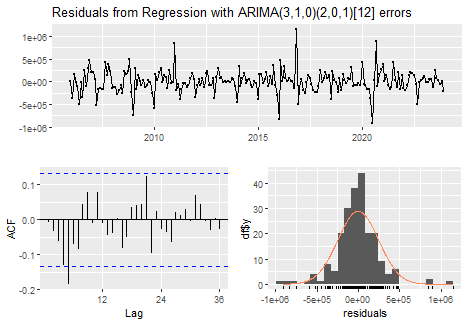
\includegraphics[width=0.8\linewidth]{plots/auto_sarimax1_metrics-1}

\begin{verbatim}

    Ljung-Box test

data:  Residuals from Regression with ARIMA(3,1,0)(2,0,1)[12] errors
Q* = 29.078, df = 18, p-value = 0.04744

Model df: 6.   Total lags used: 24
\end{verbatim}

\begin{Shaded}
\begin{Highlighting}[]
\NormalTok{r2 }\OtherTok{\textless{}{-}} \FunctionTok{sprintf}\NormalTok{(}\StringTok{"\%.3f"}\NormalTok{, }\FunctionTok{R2\_Score}\NormalTok{(fit.sarimax1, cinema\_admissions))}
\NormalTok{acc }\OtherTok{\textless{}{-}} \FunctionTok{as.data.frame.array}\NormalTok{(}\FunctionTok{accuracy}\NormalTok{(sarimax\_model1))}
\NormalTok{mae }\OtherTok{\textless{}{-}} \FunctionTok{format}\NormalTok{(acc}\SpecialCharTok{$}\NormalTok{MAE, }\AttributeTok{big.mark =} \StringTok{","}\NormalTok{, }\AttributeTok{nsmall =} \DecValTok{2}\NormalTok{, }\AttributeTok{scientific =} \ConstantTok{FALSE}\NormalTok{)}
\NormalTok{rmse }\OtherTok{\textless{}{-}} \FunctionTok{format}\NormalTok{(acc}\SpecialCharTok{$}\NormalTok{RMSE, }\AttributeTok{big.mark =} \StringTok{","}\NormalTok{, }\AttributeTok{nsmall =} \DecValTok{2}\NormalTok{, }\AttributeTok{scientific =} \ConstantTok{FALSE}\NormalTok{)}

\NormalTok{model\_performance[}\FunctionTok{nrow}\NormalTok{(model\_performance) }\SpecialCharTok{+} \DecValTok{1}\NormalTok{, ] }\OtherTok{\textless{}{-}} \FunctionTok{c}\NormalTok{(model\_name, aic, dw,}
\NormalTok{    lj\_box, r2, mae, rmse)}
\end{Highlighting}
\end{Shaded}

\begin{Shaded}
\begin{Highlighting}[]
\NormalTok{sarimax\_model2 }\OtherTok{\textless{}{-}} \FunctionTok{Arima}\NormalTok{(cinema\_admissions, }\AttributeTok{order =} \FunctionTok{c}\NormalTok{(}\DecValTok{1}\NormalTok{, }\DecValTok{0}\NormalTok{, }\DecValTok{2}\NormalTok{), }\AttributeTok{seasonal =} \FunctionTok{c}\NormalTok{(}\DecValTok{0}\NormalTok{,}
    \DecValTok{1}\NormalTok{, }\DecValTok{1}\NormalTok{), }\AttributeTok{xreg =}\NormalTok{ xreg1)}
\FunctionTok{summary}\NormalTok{(sarimax\_model2)}
\end{Highlighting}
\end{Shaded}

\begin{verbatim}
Series: cinema_admissions 
Regression with ARIMA(1,0,2)(0,1,1)[12] errors 

Coefficients:
         ar1      ma1      ma2     sma1  cinema_screening  cinema_spending
      0.9850  -0.5864  -0.2844  -0.5687            2.8262           0.1347
s.e.  0.0199   0.0694   0.0676   0.0688            0.5295           0.0017
      avg_cinema_spending_pp   cpi_all
                  -830259.32  73650.08
s.e.                46125.92  50749.25

sigma^2 = 6.126e+10:  log likelihood = -2821.25
AIC=5660.49   AICc=5661.42   BIC=5690.36

Training set error measures:
                   ME     RMSE      MAE MPE MAPE      MASE       ACF1
Training set -7119.32 235764.4 163212.9 NaN  Inf 0.0918297 0.03447954
\end{verbatim}

\begin{Shaded}
\begin{Highlighting}[]
\NormalTok{fit.sarimax2 }\OtherTok{\textless{}{-}} \FunctionTok{fitted}\NormalTok{(sarimax\_model2)}

\FunctionTok{plot}\NormalTok{(cinema\_admissions, }\AttributeTok{type =} \StringTok{"o"}\NormalTok{, }\AttributeTok{pch =} \DecValTok{16}\NormalTok{, }\AttributeTok{cex =} \FloatTok{0.6}\NormalTok{)}
\FunctionTok{lines}\NormalTok{(fit.sarimax2, }\AttributeTok{col =} \StringTok{"orange2"}\NormalTok{, }\AttributeTok{lwd =} \DecValTok{2}\NormalTok{)}
\end{Highlighting}
\end{Shaded}

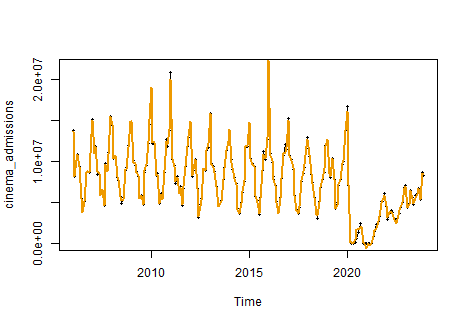
\includegraphics[width=0.8\linewidth]{plots/sarimax2-1}

\begin{Shaded}
\begin{Highlighting}[]
\NormalTok{res.sarimax\_model2 }\OtherTok{\textless{}{-}} \FunctionTok{residuals}\NormalTok{(sarimax\_model2)}
\FunctionTok{tsdisplay}\NormalTok{(res.sarimax\_model2)}
\end{Highlighting}
\end{Shaded}

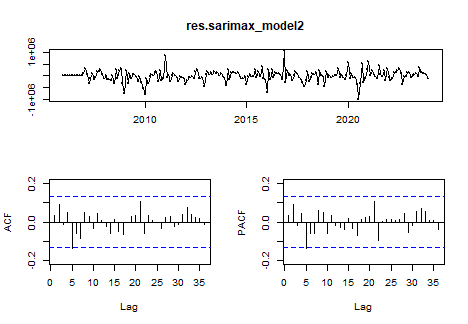
\includegraphics[width=0.8\linewidth]{plots/sarimax2-2}

\begin{Shaded}
\begin{Highlighting}[]
\FunctionTok{checkresiduals}\NormalTok{(sarimax\_model2)}
\end{Highlighting}
\end{Shaded}

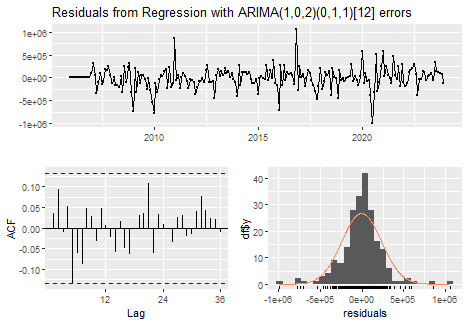
\includegraphics[width=0.8\linewidth]{plots/sarimax2-3}

\begin{verbatim}

    Ljung-Box test

data:  Residuals from Regression with ARIMA(1,0,2)(0,1,1)[12] errors
Q* = 18.114, df = 20, p-value = 0.5799

Model df: 4.   Total lags used: 24
\end{verbatim}

\begin{Shaded}
\begin{Highlighting}[]
\NormalTok{model\_name }\OtherTok{\textless{}{-}} \StringTok{"SARIMAx(1,0,2)(0,1,1)12"}
\NormalTok{aic }\OtherTok{\textless{}{-}} \FunctionTok{sprintf}\NormalTok{(}\StringTok{"\%.3f"}\NormalTok{, }\FunctionTok{AIC}\NormalTok{(sarimax\_model2))}
\NormalTok{dw }\OtherTok{\textless{}{-}} \ConstantTok{NA}
\NormalTok{lj\_box }\OtherTok{\textless{}{-}} \FunctionTok{sprintf}\NormalTok{(}\StringTok{"\%.3f"}\NormalTok{, }\FunctionTok{checkresiduals}\NormalTok{(sarimax\_model2)}\SpecialCharTok{$}\NormalTok{p.value)}
\end{Highlighting}
\end{Shaded}

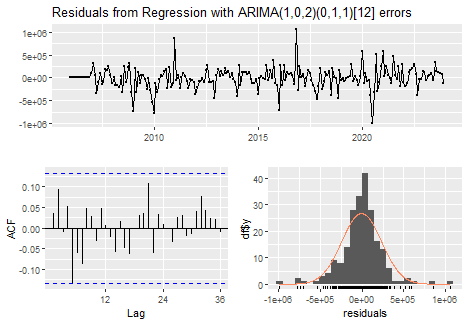
\includegraphics[width=0.8\linewidth]{plots/sarimax2_metrics-1}

\begin{verbatim}

    Ljung-Box test

data:  Residuals from Regression with ARIMA(1,0,2)(0,1,1)[12] errors
Q* = 18.114, df = 20, p-value = 0.5799

Model df: 4.   Total lags used: 24
\end{verbatim}

\begin{Shaded}
\begin{Highlighting}[]
\NormalTok{r2 }\OtherTok{\textless{}{-}} \FunctionTok{sprintf}\NormalTok{(}\StringTok{"\%.3f"}\NormalTok{, }\FunctionTok{R2\_Score}\NormalTok{(fit.sarimax2, cinema\_admissions))}
\NormalTok{acc }\OtherTok{\textless{}{-}} \FunctionTok{as.data.frame.array}\NormalTok{(}\FunctionTok{accuracy}\NormalTok{(sarimax\_model2))}
\NormalTok{mae }\OtherTok{\textless{}{-}} \FunctionTok{format}\NormalTok{(acc}\SpecialCharTok{$}\NormalTok{MAE, }\AttributeTok{big.mark =} \StringTok{","}\NormalTok{, }\AttributeTok{nsmall =} \DecValTok{2}\NormalTok{, }\AttributeTok{scientific =} \ConstantTok{FALSE}\NormalTok{)}
\NormalTok{rmse }\OtherTok{\textless{}{-}} \FunctionTok{format}\NormalTok{(acc}\SpecialCharTok{$}\NormalTok{RMSE, }\AttributeTok{big.mark =} \StringTok{","}\NormalTok{, }\AttributeTok{nsmall =} \DecValTok{2}\NormalTok{, }\AttributeTok{scientific =} \ConstantTok{FALSE}\NormalTok{)}

\NormalTok{model\_performance[}\FunctionTok{nrow}\NormalTok{(model\_performance) }\SpecialCharTok{+} \DecValTok{1}\NormalTok{, ] }\OtherTok{\textless{}{-}} \FunctionTok{c}\NormalTok{(model\_name, aic, dw,}
\NormalTok{    lj\_box, r2, mae, rmse)}
\end{Highlighting}
\end{Shaded}

\subsection{Diffusion Models}\label{diffusion-models}

\subsubsection{Bass Model (BM)}\label{bass-model-bm}

\begin{Shaded}
\begin{Highlighting}[]
\CommentTok{\# Fit the Bass Model}
\NormalTok{BM.cinema\_admissions }\OtherTok{\textless{}{-}} \FunctionTok{BM}\NormalTok{(cinema\_admissions)}
\end{Highlighting}
\end{Shaded}

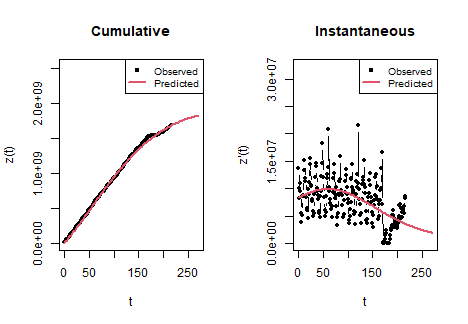
\includegraphics[width=0.8\linewidth]{plots/bass_model-1}

\begin{Shaded}
\begin{Highlighting}[]
\FunctionTok{summary}\NormalTok{(BM.cinema\_admissions)}
\end{Highlighting}
\end{Shaded}

\begin{verbatim}
Call: ( Standard Bass Model )

  BM(series = cinema_admissions)

Residuals:
      Min.   1st Qu.    Median      Mean   3rd Qu.      Max. 
-32795351 -13185860   2400549   1195905  11867557  61205017 

Coefficients:
       Estimate    Std.Error        Lower        Upper   p-value    
m 1.963262e+09 1.836356e+07 1.927270e+09 1.999254e+09 4.77e-187 ***
p 4.245253e-03 3.418230e-05 4.178257e-03 4.312249e-03 1.08e-200 ***
q 9.821809e-03 3.598327e-04 9.116550e-03 1.052707e-02  1.76e-71 ***
---
 Signif. codes:  0 '***' 0.001 '**' 0.01 '*' 0.05 '.' 0.1 ' ' 1

 Residual standard error  18656992  on  213  degrees of freedom
 Multiple R-squared:   0.999705  Residual sum of squares:  7.414175e+16
\end{verbatim}

\begin{Shaded}
\begin{Highlighting}[]
\FunctionTok{checkresiduals}\NormalTok{(BM.cinema\_admissions)}
\end{Highlighting}
\end{Shaded}

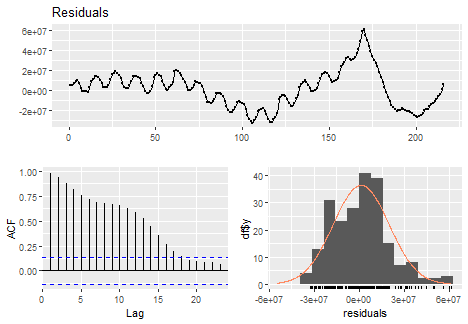
\includegraphics[width=0.8\linewidth]{plots/bass_model-2}

\begin{verbatim}

    Ljung-Box test

data:  Residuals
Q* = 1378.5, df = 10, p-value < 2.2e-16

Model df: 0.   Total lags used: 10
\end{verbatim}

\begin{Shaded}
\begin{Highlighting}[]
\FunctionTok{plot.Dimora}\NormalTok{(BM.cinema\_admissions)}
\end{Highlighting}
\end{Shaded}

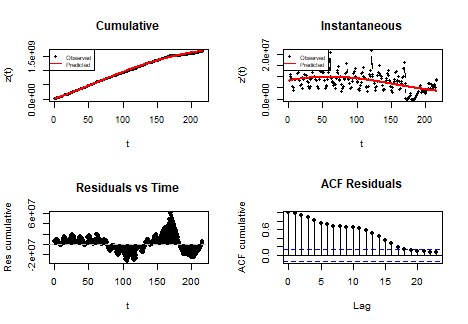
\includegraphics[width=0.8\linewidth]{plots/bass_model-3}

Future Prediction

\begin{Shaded}
\begin{Highlighting}[]
\CommentTok{\# Generate time index for observed data (2006 to 2023, monthly)}
\NormalTok{observed\_months }\OtherTok{\textless{}{-}} \FunctionTok{seq}\NormalTok{(}\FunctionTok{as.Date}\NormalTok{(}\StringTok{"2006{-}01{-}01"}\NormalTok{), }\FunctionTok{as.Date}\NormalTok{(}\StringTok{"2023{-}12{-}01"}\NormalTok{), }\AttributeTok{by =} \StringTok{"month"}\NormalTok{)}
\CommentTok{\# Generate time index for predictions (2006 to 2033, monthly)}
\CommentTok{\#predicted\_months \textless{}{-} seq(as.Date("2006{-}01{-}01"), as.Date("2033{-}12{-}01"), by = "month")}

\CommentTok{\# Set prediction horizon}
\NormalTok{forecast\_horizon }\OtherTok{\textless{}{-}} \DecValTok{60}  

\CommentTok{\# Start predictions from the first month after observed data ends}
\NormalTok{predicted\_months }\OtherTok{\textless{}{-}} \FunctionTok{seq}\NormalTok{(}\AttributeTok{from =} \FunctionTok{max}\NormalTok{(observed\_months) }\SpecialCharTok{+} \DecValTok{1}\NormalTok{,  }\CommentTok{\# Start from next month}
                         \AttributeTok{by =} \StringTok{"month"}\NormalTok{,                    }
                         \AttributeTok{length.out =}\NormalTok{ forecast\_horizon)   }
\end{Highlighting}
\end{Shaded}

\begin{Shaded}
\begin{Highlighting}[]
\CommentTok{\# Predict into the future}
\NormalTok{pred\_BM.cinema\_admissions }\OtherTok{\textless{}{-}} \FunctionTok{predict}\NormalTok{(BM.cinema\_admissions, }\AttributeTok{newx =} \DecValTok{1}\SpecialCharTok{:}\FunctionTok{length}\NormalTok{(observed\_months))}
\NormalTok{inst\_pred\_BM.cinema\_admissions }\OtherTok{\textless{}{-}} \FunctionTok{make.instantaneous}\NormalTok{(pred\_BM.cinema\_admissions)}
\end{Highlighting}
\end{Shaded}

\begin{Shaded}
\begin{Highlighting}[]
\NormalTok{model\_name }\OtherTok{\textless{}{-}} \StringTok{"Bass Model"}
\NormalTok{aic }\OtherTok{\textless{}{-}} \ConstantTok{NA}
\NormalTok{dw }\OtherTok{\textless{}{-}} \ConstantTok{NA}
\NormalTok{lj\_box }\OtherTok{\textless{}{-}} \StringTok{"\textless{} 2.2e{-}16"}
\NormalTok{r2 }\OtherTok{\textless{}{-}} \FunctionTok{sprintf}\NormalTok{(}\StringTok{"\%.3f"}\NormalTok{, }\FunctionTok{as.numeric}\NormalTok{(BM.cinema\_admissions}\SpecialCharTok{$}\NormalTok{Rsquared))}
\CommentTok{\# acc \textless{}{-} as.data.frame.array(accuracy(sarimax\_model2))}
\NormalTok{mae }\OtherTok{\textless{}{-}} \FunctionTok{format}\NormalTok{(}\FunctionTok{mean}\NormalTok{(}\FunctionTok{abs}\NormalTok{(cinema\_admissions }\SpecialCharTok{{-}}\NormalTok{ inst\_pred\_BM.cinema\_admissions)),}
    \AttributeTok{big.mark =} \StringTok{","}\NormalTok{, }\AttributeTok{nsmall =} \DecValTok{2}\NormalTok{, }\AttributeTok{scientific =} \ConstantTok{FALSE}\NormalTok{)}
\NormalTok{rmse }\OtherTok{\textless{}{-}} \FunctionTok{format}\NormalTok{(}\FunctionTok{sqrt}\NormalTok{(}\FunctionTok{mean}\NormalTok{((cinema\_admissions }\SpecialCharTok{{-}}\NormalTok{ inst\_pred\_BM.cinema\_admissions)}\SpecialCharTok{\^{}}\DecValTok{2}\NormalTok{)),}
    \AttributeTok{big.mark =} \StringTok{","}\NormalTok{, }\AttributeTok{nsmall =} \DecValTok{2}\NormalTok{, }\AttributeTok{scientific =} \ConstantTok{FALSE}\NormalTok{)}

\NormalTok{model\_performance[}\FunctionTok{nrow}\NormalTok{(model\_performance) }\SpecialCharTok{+} \DecValTok{1}\NormalTok{, ] }\OtherTok{\textless{}{-}} \FunctionTok{c}\NormalTok{(model\_name, aic, dw,}
\NormalTok{    lj\_box, r2, mae, rmse)}
\end{Highlighting}
\end{Shaded}

\begin{Shaded}
\begin{Highlighting}[]
\CommentTok{\# Predict into the future}
\NormalTok{forecast\_BM.cinema\_admissions }\OtherTok{\textless{}{-}} \FunctionTok{predict}\NormalTok{(BM.cinema\_admissions, }\AttributeTok{newx =} \DecValTok{1}\SpecialCharTok{:}\FunctionTok{length}\NormalTok{(}\FunctionTok{c}\NormalTok{(observed\_months,}
\NormalTok{    predicted\_months)))}
\NormalTok{inst\_forecast\_BM.cinema\_admissions }\OtherTok{\textless{}{-}} \FunctionTok{make.instantaneous}\NormalTok{(forecast\_BM.cinema\_admissions)}
\end{Highlighting}
\end{Shaded}

\subsubsection{GBM}\label{gbm}

\begin{Shaded}
\begin{Highlighting}[]
\CommentTok{\# GBM exponential shock}
\NormalTok{GBM.e2 }\OtherTok{\textless{}{-}} \FunctionTok{GBM}\NormalTok{(cinema\_admissions, }\AttributeTok{shock =} \StringTok{"exp"}\NormalTok{, }\AttributeTok{nshock =} \DecValTok{2}\NormalTok{, }\AttributeTok{prelimestimates =} \FunctionTok{c}\NormalTok{(}\DecValTok{1963349000}\NormalTok{,}
    \FloatTok{0.004244444}\NormalTok{, }\FloatTok{0.009822524}\NormalTok{, }\DecValTok{170}\NormalTok{, }\SpecialCharTok{{-}}\FloatTok{0.1}\NormalTok{, }\SpecialCharTok{{-}}\DecValTok{1}\NormalTok{, }\DecValTok{178}\NormalTok{, }\SpecialCharTok{{-}}\FloatTok{0.7}\NormalTok{, }\SpecialCharTok{{-}}\FloatTok{0.5}\NormalTok{))}
\end{Highlighting}
\end{Shaded}

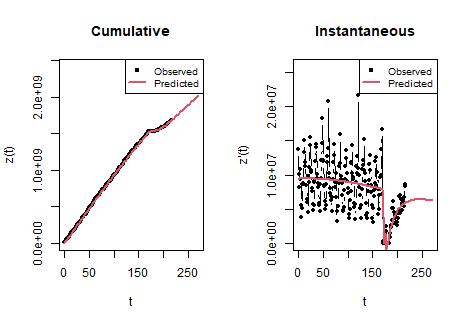
\includegraphics[width=0.8\linewidth]{plots/GBMe2-1}

\begin{Shaded}
\begin{Highlighting}[]
\CommentTok{\# m,p,q, a(starting point), b(memory of the shock), c(intensity)}
\FunctionTok{summary}\NormalTok{(GBM.e2)}
\end{Highlighting}
\end{Shaded}

\begin{verbatim}
Call: ( Generalized Bass model with 2  Exponential  shock )

  GBM(series = cinema_admissions, shock = "exp", nshock = 2, prelimestimates = c(1963349000, 
    0.004244444, 0.009822524, 170, -0.1, -1, 178, -0.7, -0.5))

Residuals:
      Min.   1st Qu.    Median      Mean   3rd Qu.      Max. 
-16755744  -4440017   -114140   -258674   3948145  17723321 

Coefficients:
           Estimate    Std.Error         Lower         Upper   p-value    
m     3.502525e+09 2.169223e+08  3.077365e+09  3.927685e+09  1.70e-38 ***
p     2.689675e-03 1.524214e-04  2.390934e-03  2.988415e-03  3.88e-43 ***
q     2.964453e-03 3.723996e-04  2.234563e-03  3.694343e-03  1.12e-13 ***
a1    1.715302e+02 7.509239e-01  1.700584e+02  1.730019e+02 1.02e-250 ***
b1   -7.729553e-02 8.319385e-02 -2.403525e-01  8.576142e-02  3.54e-01    
c1   -1.108408e+00 3.035016e-01 -1.703260e+00 -5.135557e-01  3.30e-04 ***
a2    1.778559e+02 2.047755e+00  1.738424e+02  1.818695e+02 8.05e-165 ***
b2   -2.586395e-02 1.276446e-02 -5.088183e-02 -8.460707e-04  4.40e-02   *
c2   -4.554099e-01 4.649267e-01 -1.366649e+00  4.558296e-01  3.28e-01    
---
 Signif. codes:  0 '***' 0.001 '**' 0.01 '*' 0.05 '.' 0.1 ' ' 1

 Residual standard error  7121145  on  207  degrees of freedom
 Multiple R-squared:   0.999814  Residual sum of squares:  1.049712e+16
\end{verbatim}

\begin{Shaded}
\begin{Highlighting}[]
\FunctionTok{checkresiduals}\NormalTok{(GBM.e2)}
\end{Highlighting}
\end{Shaded}

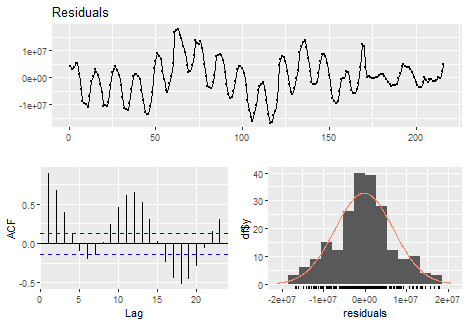
\includegraphics[width=0.8\linewidth]{plots/GBMe2-2}

\begin{verbatim}

    Ljung-Box test

data:  Residuals
Q* = 391.2, df = 10, p-value < 2.2e-16

Model df: 0.   Total lags used: 10
\end{verbatim}

\begin{Shaded}
\begin{Highlighting}[]
\FunctionTok{plot.Dimora}\NormalTok{(GBM.e2)}
\end{Highlighting}
\end{Shaded}

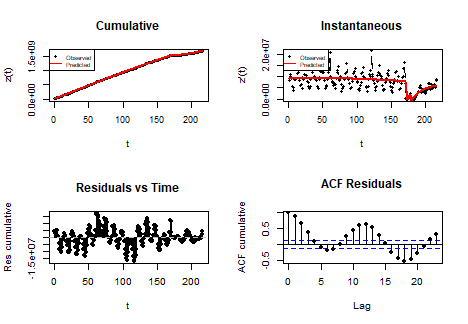
\includegraphics[width=0.8\linewidth]{plots/GBMe2-3}

\begin{Shaded}
\begin{Highlighting}[]
\CommentTok{\# Predict into the future}
\NormalTok{pred\_GBM.e2 }\OtherTok{\textless{}{-}} \FunctionTok{predict}\NormalTok{(GBM.e2, }\AttributeTok{newx =} \DecValTok{1}\SpecialCharTok{:}\FunctionTok{length}\NormalTok{(observed\_months))}
\NormalTok{inst\_pred\_GBM.e2 }\OtherTok{\textless{}{-}} \FunctionTok{make.instantaneous}\NormalTok{(pred\_GBM.e2)}
\end{Highlighting}
\end{Shaded}

\begin{Shaded}
\begin{Highlighting}[]
\NormalTok{model\_name }\OtherTok{\textless{}{-}} \StringTok{"GBMe2"}
\NormalTok{aic }\OtherTok{\textless{}{-}} \ConstantTok{NA}
\NormalTok{dw }\OtherTok{\textless{}{-}} \ConstantTok{NA}
\NormalTok{lj\_box }\OtherTok{\textless{}{-}} \StringTok{"\textless{} 2.2e{-}16"}
\NormalTok{r2 }\OtherTok{\textless{}{-}} \FunctionTok{sprintf}\NormalTok{(}\StringTok{"\%.3f"}\NormalTok{, GBM.e2}\SpecialCharTok{$}\NormalTok{Rsquared)}
\CommentTok{\# acc \textless{}{-} as.data.frame.array(accuracy(sarimax\_model2))}
\NormalTok{mae }\OtherTok{\textless{}{-}} \FunctionTok{format}\NormalTok{(}\FunctionTok{mean}\NormalTok{(}\FunctionTok{abs}\NormalTok{(cinema\_admissions }\SpecialCharTok{{-}}\NormalTok{ inst\_pred\_GBM.e2)), }\AttributeTok{big.mark =} \StringTok{","}\NormalTok{,}
    \AttributeTok{nsmall =} \DecValTok{2}\NormalTok{, }\AttributeTok{scientific =} \ConstantTok{FALSE}\NormalTok{)}
\NormalTok{rmse }\OtherTok{\textless{}{-}} \FunctionTok{format}\NormalTok{(}\FunctionTok{sqrt}\NormalTok{(}\FunctionTok{mean}\NormalTok{((cinema\_admissions }\SpecialCharTok{{-}}\NormalTok{ inst\_pred\_GBM.e2)}\SpecialCharTok{\^{}}\DecValTok{2}\NormalTok{)), }\AttributeTok{big.mark =} \StringTok{","}\NormalTok{,}
    \AttributeTok{nsmall =} \DecValTok{2}\NormalTok{, }\AttributeTok{scientific =} \ConstantTok{FALSE}\NormalTok{)}

\NormalTok{model\_performance[}\FunctionTok{nrow}\NormalTok{(model\_performance) }\SpecialCharTok{+} \DecValTok{1}\NormalTok{, ] }\OtherTok{\textless{}{-}} \FunctionTok{c}\NormalTok{(model\_name, aic, dw,}
\NormalTok{    lj\_box, r2, mae, rmse)}
\end{Highlighting}
\end{Shaded}

Future Prediction

\begin{Shaded}
\begin{Highlighting}[]
\CommentTok{\# Predict into the future}
\NormalTok{forecast\_GBM.cinema\_admissions }\OtherTok{\textless{}{-}} \FunctionTok{predict}\NormalTok{(GBM.e2, }\AttributeTok{newx =} \DecValTok{1}\SpecialCharTok{:}\FunctionTok{length}\NormalTok{(}\FunctionTok{c}\NormalTok{(observed\_months,}
\NormalTok{    predicted\_months)))}
\NormalTok{inst\_forecast\_GBM.cinema\_admissions }\OtherTok{\textless{}{-}} \FunctionTok{make.instantaneous}\NormalTok{(forecast\_GBM.cinema\_admissions)}
\end{Highlighting}
\end{Shaded}

\begin{Shaded}
\begin{Highlighting}[]
\CommentTok{\# Plot observed monthly cinema\_admissions}
\FunctionTok{plot}\NormalTok{(observed\_months, cinema\_admissions, }\AttributeTok{type =} \StringTok{"o"}\NormalTok{, }\AttributeTok{pch =} \DecValTok{16}\NormalTok{, }\AttributeTok{lty =} \DecValTok{3}\NormalTok{, }\AttributeTok{cex =} \FloatTok{0.6}\NormalTok{,}
    \AttributeTok{xlab =} \StringTok{"Time"}\NormalTok{, }\AttributeTok{ylab =} \StringTok{"Monthly Cinema Admissions"}\NormalTok{, }\AttributeTok{xlim =} \FunctionTok{range}\NormalTok{(}\FunctionTok{c}\NormalTok{(observed\_months,}
\NormalTok{        predicted\_months)), }\AttributeTok{ylim =} \FunctionTok{c}\NormalTok{(}\DecValTok{0}\NormalTok{, }\FunctionTok{max}\NormalTok{(cinema\_admissions, inst\_forecast\_GBM.cinema\_admissions)))}

\CommentTok{\# Overlay predicted instantaneous cinema\_admissions}
\FunctionTok{lines}\NormalTok{(}\FunctionTok{c}\NormalTok{(observed\_months, predicted\_months), inst\_forecast\_BM.cinema\_admissions,}
    \AttributeTok{lwd =} \DecValTok{3}\NormalTok{, }\AttributeTok{col =} \DecValTok{2}\NormalTok{)}
\FunctionTok{lines}\NormalTok{(}\FunctionTok{c}\NormalTok{(observed\_months, predicted\_months), inst\_forecast\_GBM.cinema\_admissions,}
    \AttributeTok{lwd =} \DecValTok{3}\NormalTok{, }\AttributeTok{col =} \DecValTok{3}\NormalTok{)}

\FunctionTok{legend}\NormalTok{(}\StringTok{"topright"}\NormalTok{, }\FunctionTok{c}\NormalTok{(}\StringTok{"Bass Model"}\NormalTok{, }\StringTok{"GBMe2"}\NormalTok{), }\AttributeTok{col =} \FunctionTok{c}\NormalTok{(}\DecValTok{2}\NormalTok{, }\DecValTok{3}\NormalTok{), }\AttributeTok{lty =} \FunctionTok{c}\NormalTok{(}\DecValTok{1}\NormalTok{, }\DecValTok{1}\NormalTok{),}
    \AttributeTok{lwd =} \FunctionTok{c}\NormalTok{(}\DecValTok{3}\NormalTok{, }\DecValTok{3}\NormalTok{), }\AttributeTok{merge =} \ConstantTok{TRUE}\NormalTok{, }\AttributeTok{cex =} \FloatTok{0.8}\NormalTok{)}
\end{Highlighting}
\end{Shaded}

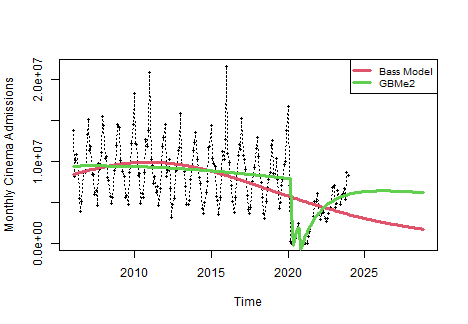
\includegraphics[width=0.8\linewidth]{plots/bm_gbm_predict-1}

\subsubsection{GBM with ARIMAx
refinement}\label{gbm-with-arimax-refinement}

\begin{Shaded}
\begin{Highlighting}[]
\CommentTok{\# SARMAX Refinement}
\NormalTok{fit\_GBM.e2 }\OtherTok{\textless{}{-}} \FunctionTok{fitted}\NormalTok{(GBM.e2)}
\CommentTok{\# inst\_fit\_GBM.cinema\_admissions\textless{}{-}}
\CommentTok{\# make.instantaneous(fit\_GBM.cinema\_admissions)}

\NormalTok{GBM.sarmax }\OtherTok{\textless{}{-}} \FunctionTok{Arima}\NormalTok{(}\FunctionTok{cumsum}\NormalTok{(cinema\_admissions), }\AttributeTok{order =} \FunctionTok{c}\NormalTok{(}\DecValTok{2}\NormalTok{, }\DecValTok{1}\NormalTok{, }\DecValTok{0}\NormalTok{), }\AttributeTok{seasonal =} \FunctionTok{list}\NormalTok{(}\AttributeTok{order =} \FunctionTok{c}\NormalTok{(}\DecValTok{0}\NormalTok{,}
    \DecValTok{1}\NormalTok{, }\DecValTok{2}\NormalTok{), }\AttributeTok{period =} \DecValTok{12}\NormalTok{), }\AttributeTok{xreg =}\NormalTok{ fit\_GBM.e2)}
\FunctionTok{summary}\NormalTok{(GBM.sarmax)}
\end{Highlighting}
\end{Shaded}

\begin{verbatim}
Series: cumsum(cinema_admissions) 
Regression with ARIMA(2,1,0)(0,1,2)[12] errors 

Coefficients:
         ar1      ar2     sma1     sma2    xreg
      0.4599  -0.1670  -0.5828  -0.1125  0.9972
s.e.  0.0705   0.0722   0.0775   0.0808  0.0792

sigma^2 = 2.424e+12:  log likelihood = -3183.6
AIC=6379.21   AICc=6379.63   BIC=6399.09

Training set error measures:
                   ME    RMSE     MAE        MPE      MAPE      MASE
Training set 47332.79 1490790 1061866 0.01764457 0.1525263 0.1363268
                     ACF1
Training set -0.001565269
\end{verbatim}

\begin{Shaded}
\begin{Highlighting}[]
\NormalTok{res.GBM.sarmax }\OtherTok{\textless{}{-}} \FunctionTok{residuals}\NormalTok{(GBM.sarmax)}
\FunctionTok{tsdisplay}\NormalTok{(res.GBM.sarmax)}
\end{Highlighting}
\end{Shaded}

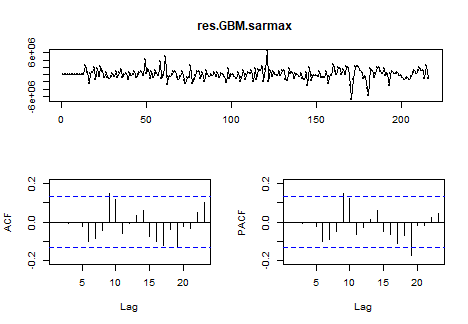
\includegraphics[width=0.8\linewidth]{plots/gbm_sarmax-1}

\begin{Shaded}
\begin{Highlighting}[]
\FunctionTok{checkresiduals}\NormalTok{(GBM.sarmax)}
\end{Highlighting}
\end{Shaded}

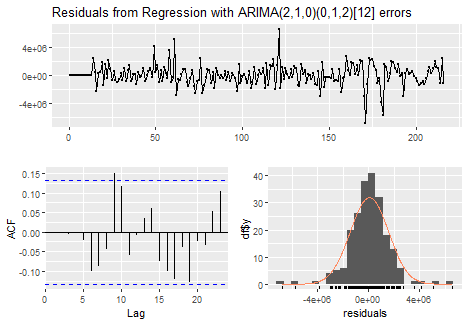
\includegraphics[width=0.8\linewidth]{plots/gbm_sarmax-2}

\begin{verbatim}

    Ljung-Box test

data:  Residuals from Regression with ARIMA(2,1,0)(0,1,2)[12] errors
Q* = 12.929, df = 6, p-value = 0.04417

Model df: 4.   Total lags used: 10
\end{verbatim}

\begin{Shaded}
\begin{Highlighting}[]
\NormalTok{fit.GBM.sarmax }\OtherTok{\textless{}{-}} \FunctionTok{fitted}\NormalTok{(GBM.sarmax)}
\NormalTok{inst\_fit.GBM.sarmax }\OtherTok{\textless{}{-}} \FunctionTok{make.instantaneous}\NormalTok{(fit.GBM.sarmax)}
\end{Highlighting}
\end{Shaded}

\begin{Shaded}
\begin{Highlighting}[]
\NormalTok{model\_name }\OtherTok{\textless{}{-}} \StringTok{"GBMe2 + ARIMAx(2,1,0)(0,1,2)12"}
\NormalTok{aic }\OtherTok{\textless{}{-}} \FunctionTok{sprintf}\NormalTok{(}\StringTok{"\%.3f"}\NormalTok{, }\FunctionTok{AIC}\NormalTok{(GBM.sarmax))}
\NormalTok{dw }\OtherTok{\textless{}{-}} \ConstantTok{NA}
\NormalTok{lj\_box }\OtherTok{\textless{}{-}} \FunctionTok{sprintf}\NormalTok{(}\StringTok{"\%.3f"}\NormalTok{, }\FunctionTok{checkresiduals}\NormalTok{(GBM.sarmax)}\SpecialCharTok{$}\NormalTok{p.value)}
\end{Highlighting}
\end{Shaded}

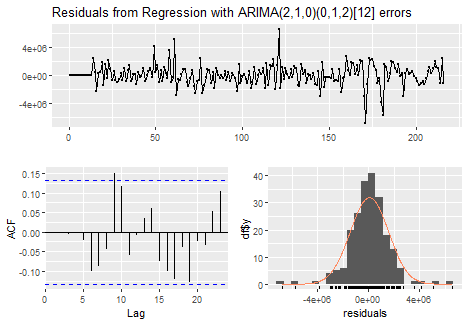
\includegraphics[width=0.8\linewidth]{plots/gbm_sarmax_metrics-1}

\begin{verbatim}

    Ljung-Box test

data:  Residuals from Regression with ARIMA(2,1,0)(0,1,2)[12] errors
Q* = 12.929, df = 6, p-value = 0.04417

Model df: 4.   Total lags used: 10
\end{verbatim}

\begin{Shaded}
\begin{Highlighting}[]
\NormalTok{r2 }\OtherTok{\textless{}{-}} \FunctionTok{sprintf}\NormalTok{(}\StringTok{"\%.3f"}\NormalTok{, }\FunctionTok{R2\_Score}\NormalTok{(}\FunctionTok{as.numeric}\NormalTok{(inst\_fit.GBM.sarmax), cinema\_admissions))}
\NormalTok{acc }\OtherTok{\textless{}{-}} \FunctionTok{as.data.frame.array}\NormalTok{(}\FunctionTok{accuracy}\NormalTok{(GBM.sarmax))}
\NormalTok{mae }\OtherTok{\textless{}{-}} \FunctionTok{format}\NormalTok{(acc}\SpecialCharTok{$}\NormalTok{MAE, }\AttributeTok{big.mark =} \StringTok{","}\NormalTok{, }\AttributeTok{nsmall =} \DecValTok{2}\NormalTok{, }\AttributeTok{scientific =} \ConstantTok{FALSE}\NormalTok{)}
\NormalTok{rmse }\OtherTok{\textless{}{-}} \FunctionTok{format}\NormalTok{(acc}\SpecialCharTok{$}\NormalTok{RMSE, }\AttributeTok{big.mark =} \StringTok{","}\NormalTok{, }\AttributeTok{nsmall =} \DecValTok{2}\NormalTok{, }\AttributeTok{scientific =} \ConstantTok{FALSE}\NormalTok{)}

\NormalTok{model\_performance[}\FunctionTok{nrow}\NormalTok{(model\_performance) }\SpecialCharTok{+} \DecValTok{1}\NormalTok{, ] }\OtherTok{\textless{}{-}} \FunctionTok{c}\NormalTok{(model\_name, aic, dw,}
\NormalTok{    lj\_box, r2, mae, rmse)}
\end{Highlighting}
\end{Shaded}

\begin{Shaded}
\begin{Highlighting}[]
\FunctionTok{plot}\NormalTok{(observed\_months, cinema\_admissions, }\AttributeTok{type =} \StringTok{"o"}\NormalTok{, }\AttributeTok{pch =} \DecValTok{16}\NormalTok{, }\AttributeTok{lty =} \DecValTok{1}\NormalTok{, }\AttributeTok{cex =} \FloatTok{0.6}\NormalTok{,}
    \AttributeTok{lwd =} \DecValTok{2}\NormalTok{, }\AttributeTok{xlab =} \StringTok{"Time"}\NormalTok{, }\AttributeTok{ylab =} \StringTok{"Monthly Cinema Admissions"}\NormalTok{, }\AttributeTok{xlim =} \FunctionTok{range}\NormalTok{(}\FunctionTok{c}\NormalTok{(observed\_months,}
\NormalTok{        predicted\_months)), }\AttributeTok{ylim =} \FunctionTok{c}\NormalTok{(}\DecValTok{0}\NormalTok{, }\FunctionTok{max}\NormalTok{(cinema\_admissions, inst\_forecast\_GBM.cinema\_admissions)))}
\FunctionTok{lines}\NormalTok{(}\FunctionTok{c}\NormalTok{(observed\_months, predicted\_months), inst\_forecast\_GBM.cinema\_admissions,}
    \AttributeTok{lwd =} \DecValTok{3}\NormalTok{, }\AttributeTok{col =} \DecValTok{3}\NormalTok{)}
\FunctionTok{lines}\NormalTok{(observed\_months, inst\_fit.GBM.sarmax, }\AttributeTok{lty =} \DecValTok{1}\NormalTok{, }\AttributeTok{lwd =} \DecValTok{1}\NormalTok{, }\AttributeTok{col =} \DecValTok{2}\NormalTok{)}
\FunctionTok{legend}\NormalTok{(}\StringTok{"topright"}\NormalTok{, }\FunctionTok{c}\NormalTok{(}\StringTok{"GBMe2"}\NormalTok{, }\StringTok{"GBMe2 + SARMAX"}\NormalTok{), }\AttributeTok{col =} \FunctionTok{c}\NormalTok{(}\DecValTok{3}\NormalTok{, }\DecValTok{2}\NormalTok{), }\AttributeTok{lty =} \FunctionTok{c}\NormalTok{(}\DecValTok{1}\NormalTok{,}
    \DecValTok{1}\NormalTok{), }\AttributeTok{lwd =} \FunctionTok{c}\NormalTok{(}\DecValTok{3}\NormalTok{, }\DecValTok{1}\NormalTok{), }\AttributeTok{merge =} \ConstantTok{TRUE}\NormalTok{, }\AttributeTok{cex =} \FloatTok{0.8}\NormalTok{)}
\end{Highlighting}
\end{Shaded}

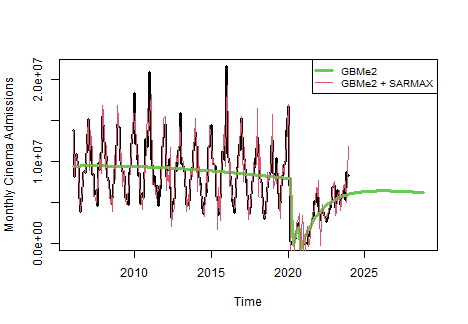
\includegraphics[width=0.8\linewidth]{plots/gbm_sarmax_plot-1}

\begin{Shaded}
\begin{Highlighting}[]
\FunctionTok{plot}\NormalTok{(observed\_months, }\FunctionTok{cumsum}\NormalTok{(cinema\_admissions), }\AttributeTok{type =} \StringTok{"b"}\NormalTok{, }\AttributeTok{pch =} \DecValTok{16}\NormalTok{, }\AttributeTok{lty =} \DecValTok{3}\NormalTok{,}
    \AttributeTok{cex =} \FloatTok{0.6}\NormalTok{, }\AttributeTok{lwd =} \DecValTok{1}\NormalTok{, }\AttributeTok{xlab =} \StringTok{"Time"}\NormalTok{, }\AttributeTok{ylab =} \StringTok{"Cumulative Monthly Cinema Admissions"}\NormalTok{,}
    \AttributeTok{xlim =} \FunctionTok{range}\NormalTok{(}\FunctionTok{c}\NormalTok{(observed\_months, predicted\_months)))}
\FunctionTok{lines}\NormalTok{(}\FunctionTok{c}\NormalTok{(observed\_months, predicted\_months), forecast\_GBM.cinema\_admissions,}
    \AttributeTok{lty =} \DecValTok{4}\NormalTok{, }\AttributeTok{lwd =} \DecValTok{2}\NormalTok{, }\AttributeTok{col =} \DecValTok{3}\NormalTok{)}
\FunctionTok{lines}\NormalTok{(observed\_months, }\FunctionTok{cumsum}\NormalTok{(inst\_fit.GBM.sarmax), }\AttributeTok{lty =} \DecValTok{4}\NormalTok{, }\AttributeTok{lwd =} \DecValTok{2}\NormalTok{, }\AttributeTok{col =} \DecValTok{2}\NormalTok{)}
\FunctionTok{legend}\NormalTok{(}\StringTok{"bottomright"}\NormalTok{, }\FunctionTok{c}\NormalTok{(}\StringTok{"GBMe2"}\NormalTok{, }\StringTok{"GBMe2 + SARMAX"}\NormalTok{), }\AttributeTok{col =} \FunctionTok{c}\NormalTok{(}\DecValTok{3}\NormalTok{, }\DecValTok{2}\NormalTok{), }\AttributeTok{lty =} \FunctionTok{c}\NormalTok{(}\DecValTok{4}\NormalTok{,}
    \DecValTok{4}\NormalTok{), }\AttributeTok{lwd =} \FunctionTok{c}\NormalTok{(}\DecValTok{2}\NormalTok{, }\DecValTok{2}\NormalTok{), }\AttributeTok{merge =} \ConstantTok{TRUE}\NormalTok{, }\AttributeTok{cex =} \FloatTok{0.8}\NormalTok{)}
\end{Highlighting}
\end{Shaded}

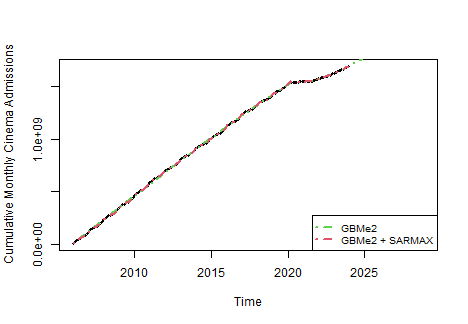
\includegraphics[width=0.8\linewidth]{plots/gbm_sarmax_cumsum-1}

!!! TODO: how to do future predictions when there are xreg???

\begin{Shaded}
\begin{Highlighting}[]
\CommentTok{\# Create future xreg using GBM model predictions}
\NormalTok{future.xreg }\OtherTok{\textless{}{-}} \FunctionTok{matrix}\NormalTok{(inst\_forecast\_GBM.cinema\_admissions, }\AttributeTok{ncol =} \DecValTok{1}\NormalTok{)}

\CommentTok{\# Forecast SARMAX with xreg}
\NormalTok{GBM.sarmax\_forecast }\OtherTok{\textless{}{-}} \FunctionTok{forecast}\NormalTok{(GBM.sarmax, }\AttributeTok{h =}\NormalTok{ forecast\_horizon, }\AttributeTok{xreg =}\NormalTok{ future.xreg)}\SpecialCharTok{$}\NormalTok{mean}
\NormalTok{inst\_GBM.sarmax\_forecast }\OtherTok{\textless{}{-}} \FunctionTok{make.instantaneous}\NormalTok{(GBM.sarmax\_forecast)}


\FunctionTok{plot}\NormalTok{(observed\_months, cinema\_admissions, }\AttributeTok{type =} \StringTok{"o"}\NormalTok{, }\AttributeTok{pch =} \DecValTok{16}\NormalTok{, }\AttributeTok{lty =} \DecValTok{1}\NormalTok{, }\AttributeTok{cex =} \FloatTok{0.6}\NormalTok{,}
    \AttributeTok{lwd =} \DecValTok{2}\NormalTok{, }\AttributeTok{xlab =} \StringTok{"Time"}\NormalTok{, }\AttributeTok{ylab =} \StringTok{"Monthly Cinema Admissions"}\NormalTok{, }\AttributeTok{xlim =} \FunctionTok{range}\NormalTok{(}\FunctionTok{c}\NormalTok{(observed\_months,}
\NormalTok{        predicted\_months)), }\AttributeTok{ylim =} \FunctionTok{c}\NormalTok{(}\DecValTok{0}\NormalTok{, }\FunctionTok{max}\NormalTok{(cinema\_admissions, inst\_forecast\_GBM.cinema\_admissions)))}

\FunctionTok{lines}\NormalTok{(observed\_months, inst\_fit.GBM.sarmax, }\AttributeTok{col =} \StringTok{"red"}\NormalTok{, }\AttributeTok{lwd =} \DecValTok{1}\NormalTok{)}
\FunctionTok{lines}\NormalTok{(}\FunctionTok{c}\NormalTok{(observed\_months, predicted\_months), inst\_GBM.sarmax\_forecast, }\AttributeTok{col =} \StringTok{"blue"}\NormalTok{,}
    \AttributeTok{lwd =} \DecValTok{2}\NormalTok{)}

\FunctionTok{legend}\NormalTok{(}\StringTok{"topright"}\NormalTok{, }\FunctionTok{c}\NormalTok{(}\StringTok{"Observed"}\NormalTok{, }\StringTok{"GBM SARMAX Refinement"}\NormalTok{, }\StringTok{"SARMAX Forecast"}\NormalTok{),}
    \AttributeTok{col =} \FunctionTok{c}\NormalTok{(}\StringTok{"black"}\NormalTok{, }\StringTok{"red"}\NormalTok{, }\StringTok{"blue"}\NormalTok{), }\AttributeTok{lty =} \FunctionTok{c}\NormalTok{(}\DecValTok{1}\NormalTok{, }\DecValTok{1}\NormalTok{, }\DecValTok{1}\NormalTok{), }\AttributeTok{lwd =} \DecValTok{2}\NormalTok{)}
\end{Highlighting}
\end{Shaded}

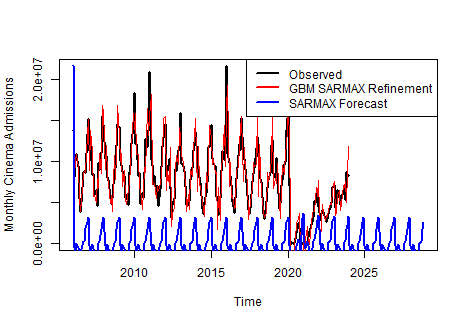
\includegraphics[width=0.8\linewidth]{plots/gbm_sarmax_future-1} !!!
TODO: obviously problematic, i need another solution for the above
problem.

\subsection{Prophet Model}\label{prophet-model}

\begin{Shaded}
\begin{Highlighting}[]
\CommentTok{\# Define COVID{-}19 lockdown periods as holidays in Prophet}
\NormalTok{lockdowns }\OtherTok{\textless{}{-}} \FunctionTok{data.frame}\NormalTok{(}
  \AttributeTok{holiday =} \FunctionTok{c}\NormalTok{(}\StringTok{"lockdown\_1"}\NormalTok{, }\StringTok{"lockdown\_2"}\NormalTok{),}
  \AttributeTok{ds =} \FunctionTok{as.Date}\NormalTok{(}\FunctionTok{c}\NormalTok{(}\StringTok{"2020{-}03{-}01"}\NormalTok{, }\StringTok{"2020{-}11{-}01"}\NormalTok{)),  }\CommentTok{\# Start dates}
  \AttributeTok{lower\_window =} \FunctionTok{c}\NormalTok{(}\DecValTok{0}\NormalTok{, }\DecValTok{0}\NormalTok{),  }\CommentTok{\# Start at the given date}
  \AttributeTok{upper\_window =} \FunctionTok{c}\NormalTok{(}\DecValTok{110}\NormalTok{, }\DecValTok{200}\NormalTok{)  }\CommentTok{\# Duration of lockdown periods}
\NormalTok{)}
\NormalTok{holiday\_season }\OtherTok{\textless{}{-}} \FunctionTok{data.frame}\NormalTok{(}
  \AttributeTok{holiday =} \StringTok{"christmas\_newyear"}\NormalTok{,}
  \AttributeTok{ds =} \FunctionTok{as.Date}\NormalTok{(}\FunctionTok{c}\NormalTok{(}\StringTok{"2006{-}12{-}01"}\NormalTok{, }\StringTok{"2007{-}12{-}01"}\NormalTok{, }\StringTok{"2008{-}12{-}01"}\NormalTok{, }\StringTok{"2009{-}12{-}01"}\NormalTok{, }
                 \StringTok{"2010{-}12{-}01"}\NormalTok{, }\StringTok{"2011{-}12{-}01"}\NormalTok{, }\StringTok{"2012{-}12{-}01"}\NormalTok{, }\StringTok{"2013{-}12{-}01"}\NormalTok{, }
                 \StringTok{"2014{-}12{-}01"}\NormalTok{, }\StringTok{"2015{-}12{-}01"}\NormalTok{, }\StringTok{"2016{-}12{-}01"}\NormalTok{, }\StringTok{"2017{-}12{-}01"}\NormalTok{, }
                 \StringTok{"2018{-}12{-}01"}\NormalTok{, }\StringTok{"2019{-}12{-}01"}\NormalTok{, }\StringTok{"2020{-}12{-}01"}\NormalTok{, }\StringTok{"2021{-}12{-}01"}\NormalTok{, }
                 \StringTok{"2022{-}12{-}01"}\NormalTok{, }\StringTok{"2023{-}12{-}01"}\NormalTok{, }\StringTok{"2024{-}12{-}01"}\NormalTok{, }\StringTok{"2025{-}12{-}01"}\NormalTok{, }
                 \StringTok{"2026{-}12{-}01"}\NormalTok{, }\StringTok{"2027{-}12{-}01"}\NormalTok{, }\StringTok{"2028{-}12{-}01"}\NormalTok{),}
               \AttributeTok{lower\_window =} \DecValTok{0}\NormalTok{, }\AttributeTok{upper\_window =} \DecValTok{45}\NormalTok{)}
\NormalTok{)}
\NormalTok{ferragosto }\OtherTok{\textless{}{-}} \FunctionTok{data.frame}\NormalTok{(}
  \AttributeTok{holiday =} \StringTok{"ferragosto"}\NormalTok{,}
  \AttributeTok{ds =} \FunctionTok{as.Date}\NormalTok{(}\FunctionTok{c}\NormalTok{(}\StringTok{"2006{-}08{-}01"}\NormalTok{, }\StringTok{"2007{-}08{-}01"}\NormalTok{, }\StringTok{"2008{-}08{-}01"}\NormalTok{, }\StringTok{"2009{-}08{-}01"}\NormalTok{, }
                 \StringTok{"2010{-}08{-}01"}\NormalTok{, }\StringTok{"2011{-}08{-}01"}\NormalTok{, }\StringTok{"2012{-}08{-}01"}\NormalTok{, }\StringTok{"2013{-}08{-}01"}\NormalTok{, }
                 \StringTok{"2014{-}08{-}01"}\NormalTok{, }\StringTok{"2015{-}08{-}01"}\NormalTok{, }\StringTok{"2016{-}08{-}01"}\NormalTok{, }\StringTok{"2017{-}08{-}01"}\NormalTok{, }
                 \StringTok{"2018{-}08{-}01"}\NormalTok{, }\StringTok{"2019{-}08{-}01"}\NormalTok{, }\StringTok{"2020{-}08{-}01"}\NormalTok{, }\StringTok{"2021{-}08{-}01"}\NormalTok{, }
                 \StringTok{"2022{-}08{-}01"}\NormalTok{, }\StringTok{"2023{-}08{-}01"}\NormalTok{, }\StringTok{"2024{-}08{-}01"}\NormalTok{, }\StringTok{"2025{-}08{-}01"}\NormalTok{, }
                 \StringTok{"2026{-}08{-}01"}\NormalTok{, }\StringTok{"2027{-}08{-}01"}\NormalTok{, }\StringTok{"2028{-}08{-}01"}\NormalTok{),}
               \AttributeTok{lower\_window =} \DecValTok{0}\NormalTok{, }\AttributeTok{upper\_window =} \DecValTok{30}\NormalTok{)}
\NormalTok{)}

\NormalTok{holidays }\OtherTok{\textless{}{-}} \FunctionTok{bind\_rows}\NormalTok{(lockdowns, holiday\_season, ferragosto)}

\CommentTok{\# Create a Date column}
\NormalTok{ott\_cinema\_monthly}\SpecialCharTok{$}\NormalTok{ds }\OtherTok{\textless{}{-}} \FunctionTok{as.Date}\NormalTok{(}\FunctionTok{paste}\NormalTok{(ott\_cinema\_monthly}\SpecialCharTok{$}\NormalTok{Year, }
                                       \FunctionTok{rep}\NormalTok{(}\DecValTok{1}\SpecialCharTok{:}\DecValTok{12}\NormalTok{, }\AttributeTok{length.out =} \FunctionTok{nrow}\NormalTok{(ott\_cinema\_monthly)), }
                                       \StringTok{"01"}\NormalTok{, }\AttributeTok{sep =} \StringTok{"{-}"}\NormalTok{))}

\CommentTok{\# create the Prophet dataframe}
\NormalTok{prophet\_data }\OtherTok{\textless{}{-}} \FunctionTok{data.frame}\NormalTok{(}\AttributeTok{ds =}\NormalTok{ ott\_cinema\_monthly}\SpecialCharTok{$}\NormalTok{ds, }
                           \AttributeTok{y =}\NormalTok{ ott\_cinema\_monthly}\SpecialCharTok{$}\NormalTok{cinema\_admissions)}
\end{Highlighting}
\end{Shaded}

\begin{Shaded}
\begin{Highlighting}[]
\CommentTok{\# Fit Prophet model with lockdown effects}
\NormalTok{prophet\_model }\OtherTok{\textless{}{-}} \FunctionTok{prophet}\NormalTok{(}\AttributeTok{holidays =}\NormalTok{ holidays, }\AttributeTok{yearly.seasonality =} \ConstantTok{TRUE}\NormalTok{,}
    \AttributeTok{seasonality.mode =} \StringTok{"multiplicative"}\NormalTok{, }\AttributeTok{changepoint.prior.scale =} \FloatTok{0.15}\NormalTok{,}
    \AttributeTok{changepoint.range =} \FloatTok{0.85}\NormalTok{)}
\NormalTok{prophet\_model }\OtherTok{\textless{}{-}} \FunctionTok{fit.prophet}\NormalTok{(prophet\_model, prophet\_data)}

\CommentTok{\# summary(prophet\_model)}
\end{Highlighting}
\end{Shaded}

\begin{Shaded}
\begin{Highlighting}[]
\CommentTok{\# Generate future dates future \textless{}{-} make\_future\_dataframe(prophet\_model,}
\CommentTok{\# periods = 12*5, freq = \textquotesingle{}month\textquotesingle{}, include\_history = TRUE)}

\CommentTok{\# Predict future values}
\NormalTok{prophet\_predict }\OtherTok{\textless{}{-}} \FunctionTok{predict}\NormalTok{(prophet\_model, prophet\_data)}
\NormalTok{prophet\_data}\SpecialCharTok{$}\NormalTok{prophet\_predict }\OtherTok{\textless{}{-}}\NormalTok{ prophet\_predict}\SpecialCharTok{$}\NormalTok{yhat}
\end{Highlighting}
\end{Shaded}

\begin{Shaded}
\begin{Highlighting}[]
\CommentTok{\# dyplot.prophet(prophet\_model, prophet\_predict)}
\end{Highlighting}
\end{Shaded}

\begin{Shaded}
\begin{Highlighting}[]
\CommentTok{\# Plot the forecast with lockdown effects}
\FunctionTok{plot}\NormalTok{(prophet\_model, prophet\_predict) }\SpecialCharTok{+} \FunctionTok{add\_changepoints\_to\_plot}\NormalTok{(prophet\_model)}
\end{Highlighting}
\end{Shaded}

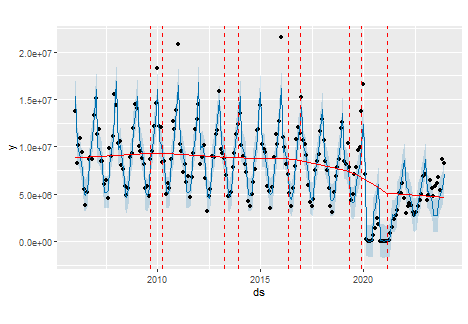
\includegraphics[width=0.8\linewidth]{plots/plot_prophet_predict-1}

\begin{Shaded}
\begin{Highlighting}[]
\FunctionTok{prophet\_plot\_components}\NormalTok{(prophet\_model, prophet\_predict)}
\end{Highlighting}
\end{Shaded}

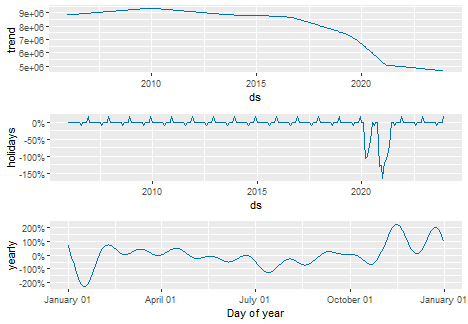
\includegraphics[width=0.8\linewidth]{plots/prophet_plot_components-1}

\begin{Shaded}
\begin{Highlighting}[]
\CommentTok{\# Generate residuals}
\NormalTok{prophet\_residuals }\OtherTok{\textless{}{-}}\NormalTok{ prophet\_data}\SpecialCharTok{$}\NormalTok{y }\SpecialCharTok{{-}}\NormalTok{ prophet\_data}\SpecialCharTok{$}\NormalTok{prophet\_predict}
\NormalTok{prophet\_data}\SpecialCharTok{$}\NormalTok{prophet\_residuals }\OtherTok{\textless{}{-}}\NormalTok{ prophet\_residuals}

\FunctionTok{checkresiduals}\NormalTok{(prophet\_residuals)}
\end{Highlighting}
\end{Shaded}

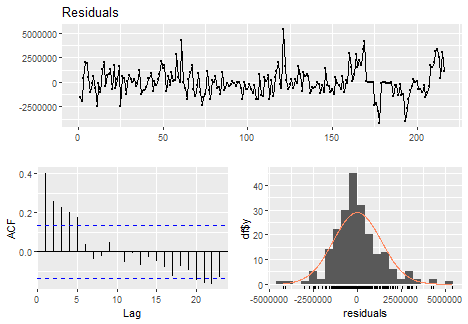
\includegraphics[width=0.8\linewidth]{plots/prophet_residuals-1}

\begin{verbatim}

    Ljung-Box test

data:  Residuals
Q* = 78.103, df = 10, p-value = 1.181e-12

Model df: 0.   Total lags used: 10
\end{verbatim}

\begin{Shaded}
\begin{Highlighting}[]
\NormalTok{model\_name }\OtherTok{\textless{}{-}} \StringTok{"Prophet"}
\NormalTok{aic }\OtherTok{\textless{}{-}} \ConstantTok{NA}
\NormalTok{dw }\OtherTok{\textless{}{-}} \ConstantTok{NA}
\NormalTok{lj\_box }\OtherTok{\textless{}{-}} \FunctionTok{sprintf}\NormalTok{(}\StringTok{"\%.3e"}\NormalTok{, }\FunctionTok{checkresiduals}\NormalTok{(prophet\_residuals)}\SpecialCharTok{$}\NormalTok{p.value)}
\end{Highlighting}
\end{Shaded}

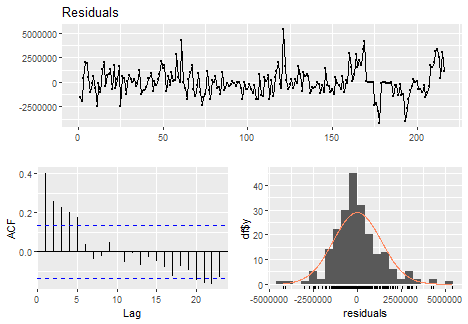
\includegraphics[width=0.8\linewidth]{plots/prophet_metrics-1}

\begin{verbatim}

    Ljung-Box test

data:  Residuals
Q* = 78.103, df = 10, p-value = 1.181e-12

Model df: 0.   Total lags used: 10
\end{verbatim}

\begin{Shaded}
\begin{Highlighting}[]
\NormalTok{r2 }\OtherTok{\textless{}{-}} \FunctionTok{sprintf}\NormalTok{(}\StringTok{"\%.3f"}\NormalTok{, }\FunctionTok{R2\_Score}\NormalTok{(prophet\_data}\SpecialCharTok{$}\NormalTok{prophet\_predict, prophet\_data}\SpecialCharTok{$}\NormalTok{y))}
\NormalTok{mae }\OtherTok{\textless{}{-}} \FunctionTok{format}\NormalTok{(}\FunctionTok{mean}\NormalTok{(}\FunctionTok{abs}\NormalTok{(prophet\_residuals)), }\AttributeTok{big.mark =} \StringTok{","}\NormalTok{, }\AttributeTok{nsmall =} \DecValTok{2}\NormalTok{, }\AttributeTok{scientific =} \ConstantTok{FALSE}\NormalTok{)}
\NormalTok{rmse }\OtherTok{\textless{}{-}} \FunctionTok{format}\NormalTok{(}\FunctionTok{sqrt}\NormalTok{(}\FunctionTok{mean}\NormalTok{((prophet\_residuals)}\SpecialCharTok{\^{}}\DecValTok{2}\NormalTok{)), }\AttributeTok{big.mark =} \StringTok{","}\NormalTok{, }\AttributeTok{nsmall =} \DecValTok{2}\NormalTok{,}
    \AttributeTok{scientific =} \ConstantTok{FALSE}\NormalTok{)}

\NormalTok{model\_performance[}\FunctionTok{nrow}\NormalTok{(model\_performance) }\SpecialCharTok{+} \DecValTok{1}\NormalTok{, ] }\OtherTok{\textless{}{-}} \FunctionTok{c}\NormalTok{(model\_name, aic, dw,}
\NormalTok{    lj\_box, r2, mae, rmse)}
\end{Highlighting}
\end{Shaded}

\subsubsection{Prophet with ARIMA
refinement}\label{prophet-with-arima-refinement}

\begin{Shaded}
\begin{Highlighting}[]
\NormalTok{prres.arima }\OtherTok{\textless{}{-}} \FunctionTok{auto.arima}\NormalTok{(prophet\_residuals)}
\FunctionTok{summary}\NormalTok{(prres.arima)}
\end{Highlighting}
\end{Shaded}

\begin{verbatim}
Series: prophet_residuals 
ARIMA(4,0,0) with zero mean 

Coefficients:
         ar1     ar2     ar3     ar4
      0.3342  0.0776  0.0854  0.0736
s.e.  0.0678  0.0722  0.0723  0.0697

sigma^2 = 1.501e+12:  log likelihood = -3332.62
AIC=6675.23   AICc=6675.52   BIC=6692.11

Training set error measures:
                   ME    RMSE      MAE      MPE    MAPE      MASE         ACF1
Training set 11818.15 1213740 929204.3 62.96382 252.077 0.8462508 -0.004008333
\end{verbatim}

\begin{Shaded}
\begin{Highlighting}[]
\NormalTok{fit.prres.arima }\OtherTok{\textless{}{-}} \FunctionTok{fitted}\NormalTok{(prres.arima)}

\NormalTok{res.prres.arima }\OtherTok{\textless{}{-}} \FunctionTok{residuals}\NormalTok{(prres.arima)}
\FunctionTok{tsdisplay}\NormalTok{(res.prres.arima)}
\end{Highlighting}
\end{Shaded}

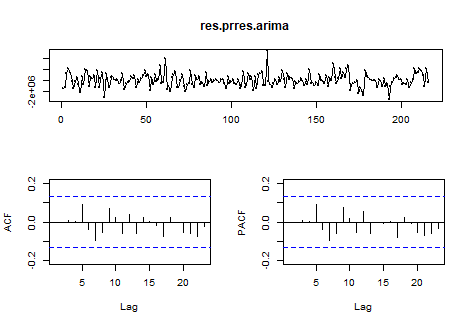
\includegraphics[width=0.8\linewidth]{plots/prophet_residuals_arima-1}

\begin{Shaded}
\begin{Highlighting}[]
\NormalTok{prophet\_data}\SpecialCharTok{$}\NormalTok{combined\_predict }\OtherTok{\textless{}{-}}\NormalTok{ prophet\_data}\SpecialCharTok{$}\NormalTok{prophet\_predict }\SpecialCharTok{+}\NormalTok{ fit.prres.arima}
\end{Highlighting}
\end{Shaded}

\begin{Shaded}
\begin{Highlighting}[]
\FunctionTok{plot}\NormalTok{(ott\_cinema\_monthly}\SpecialCharTok{$}\NormalTok{ds, ott\_cinema\_monthly}\SpecialCharTok{$}\NormalTok{cinema\_admissions, }\AttributeTok{type =} \StringTok{"o"}\NormalTok{,}
    \AttributeTok{pch =} \DecValTok{16}\NormalTok{, }\AttributeTok{cex =} \FloatTok{0.6}\NormalTok{, }\AttributeTok{xlab =} \StringTok{"Date"}\NormalTok{, }\AttributeTok{ylab =} \StringTok{"Cinema Admissions"}\NormalTok{)}

\FunctionTok{lines}\NormalTok{(ott\_cinema\_monthly}\SpecialCharTok{$}\NormalTok{ds, prophet\_data}\SpecialCharTok{$}\NormalTok{prophet\_predict, }\AttributeTok{col =} \StringTok{"orange2"}\NormalTok{,}
    \AttributeTok{lwd =} \DecValTok{2}\NormalTok{)}
\FunctionTok{lines}\NormalTok{(ott\_cinema\_monthly}\SpecialCharTok{$}\NormalTok{ds, prophet\_data}\SpecialCharTok{$}\NormalTok{combined\_predict, }\AttributeTok{col =} \StringTok{"purple2"}\NormalTok{,}
    \AttributeTok{lwd =} \DecValTok{2}\NormalTok{)}

\FunctionTok{legend}\NormalTok{(}\StringTok{"topright"}\NormalTok{, }\FunctionTok{c}\NormalTok{(}\StringTok{"Prophet"}\NormalTok{, }\StringTok{"Prophet + SARIMA"}\NormalTok{), }\AttributeTok{col =} \FunctionTok{c}\NormalTok{(}\StringTok{"orange2"}\NormalTok{, }\StringTok{"purple2"}\NormalTok{),}
    \AttributeTok{lty =} \FunctionTok{c}\NormalTok{(}\DecValTok{1}\NormalTok{, }\DecValTok{1}\NormalTok{), }\AttributeTok{lwd =} \DecValTok{2}\NormalTok{)}
\end{Highlighting}
\end{Shaded}

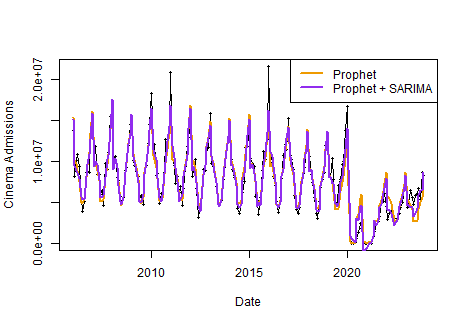
\includegraphics[width=0.8\linewidth]{plots/plot_prophet_residuals_arima-1}

\begin{Shaded}
\begin{Highlighting}[]
\CommentTok{\# Generate residuals}
\NormalTok{prophet.arima\_residuals }\OtherTok{\textless{}{-}}\NormalTok{ prophet\_data}\SpecialCharTok{$}\NormalTok{y }\SpecialCharTok{{-}}\NormalTok{ prophet\_data}\SpecialCharTok{$}\NormalTok{combined\_predict}

\NormalTok{prophet\_data}\SpecialCharTok{$}\NormalTok{combined\_residuals }\OtherTok{\textless{}{-}}\NormalTok{ prophet.arima\_residuals}

\FunctionTok{checkresiduals}\NormalTok{(prophet.arima\_residuals)}
\end{Highlighting}
\end{Shaded}

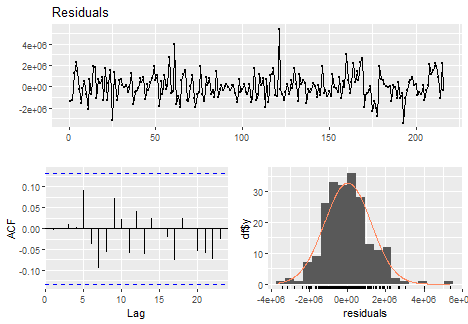
\includegraphics[width=0.8\linewidth]{plots/prophet_arima_residuals-1}

\begin{verbatim}

    Ljung-Box test

data:  Residuals
Q* = 6.4027, df = 10, p-value = 0.7804

Model df: 0.   Total lags used: 10
\end{verbatim}

\begin{Shaded}
\begin{Highlighting}[]
\NormalTok{model\_name }\OtherTok{\textless{}{-}} \StringTok{"Prophet + ARIMA"}
\NormalTok{aic }\OtherTok{\textless{}{-}} \ConstantTok{NA}
\NormalTok{dw }\OtherTok{\textless{}{-}} \ConstantTok{NA}
\NormalTok{lj\_box }\OtherTok{\textless{}{-}} \FunctionTok{sprintf}\NormalTok{(}\StringTok{"\%.3f"}\NormalTok{, }\FunctionTok{checkresiduals}\NormalTok{(prophet\_data}\SpecialCharTok{$}\NormalTok{combined\_residuals)}\SpecialCharTok{$}\NormalTok{p.value)}
\end{Highlighting}
\end{Shaded}

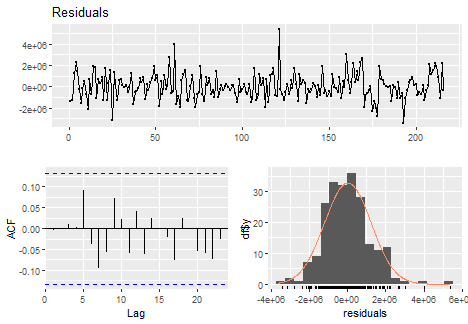
\includegraphics[width=0.8\linewidth]{plots/prophet_arima_metrics-1}

\begin{verbatim}

    Ljung-Box test

data:  Residuals
Q* = 6.4027, df = 10, p-value = 0.7804

Model df: 0.   Total lags used: 10
\end{verbatim}

\begin{Shaded}
\begin{Highlighting}[]
\NormalTok{r2 }\OtherTok{\textless{}{-}} \FunctionTok{sprintf}\NormalTok{(}\StringTok{"\%.3f"}\NormalTok{, }\FunctionTok{R2\_Score}\NormalTok{(prophet\_data}\SpecialCharTok{$}\NormalTok{combined\_predict, prophet\_data}\SpecialCharTok{$}\NormalTok{y))}
\NormalTok{mae }\OtherTok{\textless{}{-}} \FunctionTok{format}\NormalTok{(}\FunctionTok{mean}\NormalTok{(}\FunctionTok{abs}\NormalTok{(prophet\_data}\SpecialCharTok{$}\NormalTok{combined\_residuals)), }\AttributeTok{big.mark =} \StringTok{","}\NormalTok{,}
    \AttributeTok{nsmall =} \DecValTok{2}\NormalTok{, }\AttributeTok{scientific =} \ConstantTok{FALSE}\NormalTok{)}
\NormalTok{rmse }\OtherTok{\textless{}{-}} \FunctionTok{format}\NormalTok{(}\FunctionTok{sqrt}\NormalTok{(}\FunctionTok{mean}\NormalTok{((prophet\_data}\SpecialCharTok{$}\NormalTok{combined\_residuals)}\SpecialCharTok{\^{}}\DecValTok{2}\NormalTok{)), }\AttributeTok{big.mark =} \StringTok{","}\NormalTok{,}
    \AttributeTok{nsmall =} \DecValTok{2}\NormalTok{, }\AttributeTok{scientific =} \ConstantTok{FALSE}\NormalTok{)}

\NormalTok{model\_performance[}\FunctionTok{nrow}\NormalTok{(model\_performance) }\SpecialCharTok{+} \DecValTok{1}\NormalTok{, ] }\OtherTok{\textless{}{-}} \FunctionTok{c}\NormalTok{(model\_name, aic, dw,}
\NormalTok{    lj\_box, r2, mae, rmse)}
\end{Highlighting}
\end{Shaded}

\subsection{Exponential Smoothing}\label{exponential-smoothing}

\subsubsection{Holt-Winters method (for Trend and
Seasonality)}\label{holt-winters-method-for-trend-and-seasonality}

\begin{Shaded}
\begin{Highlighting}[]
\NormalTok{hw.cinema\_admissions }\OtherTok{\textless{}{-}} \FunctionTok{hw}\NormalTok{(cinema\_admissions, }\AttributeTok{seasonal =} \StringTok{"additive"}\NormalTok{)}


\FunctionTok{summary}\NormalTok{(hw.cinema\_admissions)}
\end{Highlighting}
\end{Shaded}

\begin{verbatim}

Forecast method: Holt-Winters' additive method

Model Information:
Holt-Winters' additive method 

Call:
hw(y = cinema_admissions, seasonal = "additive")

  Smoothing parameters:
    alpha = 0.7404 
    beta  = 1e-04 
    gamma = 1e-04 

  Initial states:
    l = 9169380.6501 
    b = 49001.19 
    s = 3696598 1749141 634656.7 -597404.5 -3094459 -3658436
           -3482387 -1529110 -532336.9 211025.5 903663 5699050

  sigma:  1733522

     AIC     AICc      BIC 
7384.404 7387.495 7441.784 

Error measures:
                    ME    RMSE     MAE MPE MAPE      MASE      ACF1
Training set -90448.17 1668083 1248623 NaN  Inf 0.7025221 0.0226788

Forecasts:
         Point Forecast      Lo 80    Hi 80      Lo 95    Hi 95
Jan 2024       10844047  8622448.9 13065645  7446405.9 14241688
Feb 2024        6095348  3330940.4  8859757  1867551.2 10323146
Mar 2024        5450186  2233178.8  8667194   530198.0 10370174
Apr 2024        4753858  1140404.2  8367313  -772442.9 10280160
May 2024        3803793  -166811.4  7774397 -2268722.3  9876308
Jun 2024        1897661 -2400603.0  6195926 -4675966.7  8471289
Jul 2024        1768992 -2833745.0  6371729 -5270286.7  8808270
Aug 2024        2379760 -2508596.7  7268116 -5096336.2  9855855
Sep 2024        4923637  -234618.3 10081893 -2965233.8 12812508
Oct 2024        6202615   787829.4 11617401 -2078585.0 14483815
Nov 2024        7364592  1704827.4 13024357 -1291271.3 16020456
Dec 2024        9358782  3464148.5 15253416   343717.9 18373847
Jan 2025       11408617  5288000.5 17529233  2047942.1 20769291
Feb 2025        6659918   321371.4 12998465 -3034052.5 16353888
Mar 2025        6014756  -534529.6 12564041 -4001511.8 16031023
Apr 2025        5318428 -1435077.3 12071933 -5010167.1 15647023
May 2025        4368362 -2583418.9 11320144 -6263469.6 15000194
Jun 2025        2462231 -4682377.2  9606839 -8464504.3 13388966
Jul 2025        2333561 -4998854.4  9665977 -8880400.8 13547523
Aug 2025        2944329 -4571251.1 10459909 -8549759.0 14438417
Sep 2025        5488207 -2206226.8 13182640 -6279413.8 17255827
Oct 2025        6767185 -1102084.7 14636454 -5267824.2 18802193
Nov 2025        7929162  -111187.9 15969512 -4367492.0 20225816
Dec 2025        9923352  1715442.1 18131262 -2629562.9 22476267
\end{verbatim}

\begin{Shaded}
\begin{Highlighting}[]
\FunctionTok{autoplot}\NormalTok{(hw.cinema\_admissions) }\SpecialCharTok{+} \FunctionTok{autolayer}\NormalTok{(}\FunctionTok{fitted}\NormalTok{(hw.cinema\_admissions),}
    \AttributeTok{series =} \StringTok{"Holt{-}Winters\textquotesingle{} additive"}\NormalTok{) }\SpecialCharTok{+} \FunctionTok{ylab}\NormalTok{(}\StringTok{"Cinema Admissions"}\NormalTok{) }\SpecialCharTok{+} \FunctionTok{xlab}\NormalTok{(}\StringTok{"Year"}\NormalTok{)}
\end{Highlighting}
\end{Shaded}

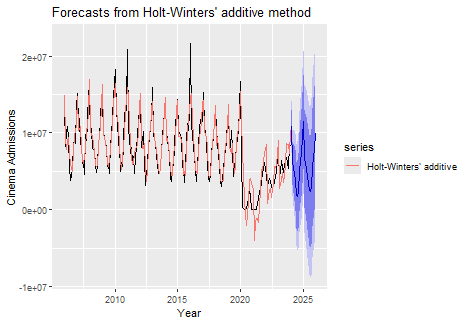
\includegraphics[width=0.8\linewidth]{plots/hw_exponential-1}

\begin{Shaded}
\begin{Highlighting}[]
\FunctionTok{checkresiduals}\NormalTok{(hw.cinema\_admissions)}
\end{Highlighting}
\end{Shaded}

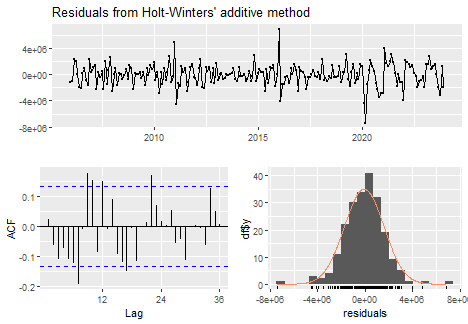
\includegraphics[width=0.8\linewidth]{plots/hw_exponential-2}

\begin{verbatim}

    Ljung-Box test

data:  Residuals from Holt-Winters' additive method
Q* = 63.089, df = 24, p-value = 2.311e-05

Model df: 0.   Total lags used: 24
\end{verbatim}

\begin{Shaded}
\begin{Highlighting}[]
\NormalTok{model\_name }\OtherTok{\textless{}{-}} \StringTok{"Holt{-}Winters Exponential"}
\NormalTok{aic }\OtherTok{\textless{}{-}} \FunctionTok{sprintf}\NormalTok{(}\StringTok{"\%.3f"}\NormalTok{, hw.cinema\_admissions}\SpecialCharTok{$}\NormalTok{model}\SpecialCharTok{$}\NormalTok{aic)}
\NormalTok{dw }\OtherTok{\textless{}{-}} \ConstantTok{NA}
\NormalTok{lj\_box }\OtherTok{\textless{}{-}} \FunctionTok{sprintf}\NormalTok{(}\StringTok{"\%.3e"}\NormalTok{, }\FunctionTok{checkresiduals}\NormalTok{(hw.cinema\_admissions)}\SpecialCharTok{$}\NormalTok{p.value)}
\end{Highlighting}
\end{Shaded}

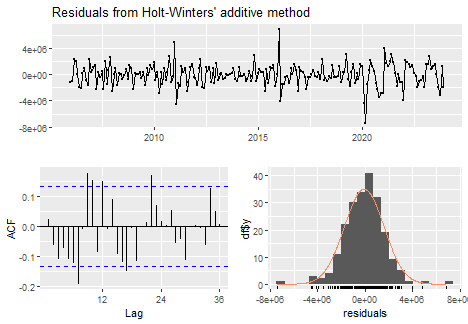
\includegraphics[width=0.8\linewidth]{plots/hw_exponential_metrics-1}

\begin{verbatim}

    Ljung-Box test

data:  Residuals from Holt-Winters' additive method
Q* = 63.089, df = 24, p-value = 2.311e-05

Model df: 0.   Total lags used: 24
\end{verbatim}

\begin{Shaded}
\begin{Highlighting}[]
\NormalTok{r2 }\OtherTok{\textless{}{-}} \FunctionTok{sprintf}\NormalTok{(}\StringTok{"\%.3f"}\NormalTok{, }\FunctionTok{R2\_Score}\NormalTok{(hw.cinema\_admissions}\SpecialCharTok{$}\NormalTok{fitted, cinema\_admissions))}
\NormalTok{acc }\OtherTok{\textless{}{-}} \FunctionTok{as.data.frame.array}\NormalTok{(}\FunctionTok{accuracy}\NormalTok{(hw.cinema\_admissions))}
\NormalTok{mae }\OtherTok{\textless{}{-}} \FunctionTok{format}\NormalTok{(acc}\SpecialCharTok{$}\NormalTok{MAE, }\AttributeTok{big.mark =} \StringTok{","}\NormalTok{, }\AttributeTok{nsmall =} \DecValTok{2}\NormalTok{, }\AttributeTok{scientific =} \ConstantTok{FALSE}\NormalTok{)}
\NormalTok{rmse }\OtherTok{\textless{}{-}} \FunctionTok{format}\NormalTok{(acc}\SpecialCharTok{$}\NormalTok{RMSE, }\AttributeTok{big.mark =} \StringTok{","}\NormalTok{, }\AttributeTok{nsmall =} \DecValTok{2}\NormalTok{, }\AttributeTok{scientific =} \ConstantTok{FALSE}\NormalTok{)}

\NormalTok{model\_performance[}\FunctionTok{nrow}\NormalTok{(model\_performance) }\SpecialCharTok{+} \DecValTok{1}\NormalTok{, ] }\OtherTok{\textless{}{-}} \FunctionTok{c}\NormalTok{(model\_name, aic, dw,}
\NormalTok{    lj\_box, r2, mae, rmse)}
\end{Highlighting}
\end{Shaded}

\begin{Shaded}
\begin{Highlighting}[]
\NormalTok{model\_performance}
\end{Highlighting}
\end{Shaded}

\begin{verbatim}
                            Model      AIC DW_Test Ljung_Box_pval    R2
1                     TSLM - Full 6054.269   1.065           <NA> 0.995
2                 TSLM - Stepwise 6050.035   1.064           <NA> 0.995
3           ARIMA(2,1,2)(1,1,1)12 6425.542    <NA>          0.077 0.828
4                      auto.ARIMA 6448.711    <NA>          0.108 0.828
5                     auto.ARIMAx 5974.656    <NA>          0.047 0.996
6         SARIMAx(1,0,2)(0,1,1)12 5660.495    <NA>          0.580 0.996
7                      Bass Model     <NA>    <NA>      < 2.2e-16 1.000
8                           GBMe2     <NA>    <NA>      < 2.2e-16 1.000
9  GBMe2 + ARIMAx(2,1,0)(0,1,2)12 6379.206    <NA>          0.044 0.718
10                        Prophet     <NA>    <NA>      1.181e-12 0.885
11                Prophet + ARIMA     <NA>    <NA>          0.780 0.907
12       Holt-Winters Exponential 7384.404    <NA>      2.311e-05 0.824
            MAE         RMSE
1    193,057.61   267,895.01
2    195,166.90   268,992.46
3  1,174,836.65 1,644,854.58
4  1,158,030.22 1,647,445.01
5    170,544.06   245,186.45
6    163,212.89   235,764.35
7  2,772,250.27 3,480,549.43
8  2,307,165.36 3,106,753.77
9  1,061,865.94 1,490,790.20
10   975,508.94 1,348,348.68
11   929,204.32 1,213,740.28
12 1,248,622.75 1,668,082.59
\end{verbatim}

\section{3) Cross-Validation}\label{cross-validation}

\subsection{Cross-Validation for Prophet +
ARIMA}\label{cross-validation-for-prophet-arima}

\begin{Shaded}
\begin{Highlighting}[]
\NormalTok{initial }\OtherTok{\textless{}{-}} \DecValTok{120}  \CommentTok{\# 10 years of training}
\NormalTok{horizon }\OtherTok{\textless{}{-}} \DecValTok{12}  \CommentTok{\# forecast 12 months}
\NormalTok{step }\OtherTok{\textless{}{-}} \DecValTok{6}  \CommentTok{\# slide window every 6 months}

\NormalTok{n }\OtherTok{\textless{}{-}} \FunctionTok{nrow}\NormalTok{(prophet\_data)}
\NormalTok{cutoffs }\OtherTok{\textless{}{-}} \FunctionTok{seq}\NormalTok{(}\AttributeTok{from =}\NormalTok{ initial, }\AttributeTok{to =}\NormalTok{ n }\SpecialCharTok{{-}}\NormalTok{ horizon, }\AttributeTok{by =}\NormalTok{ step)}

\CommentTok{\# Store metrics}
\NormalTok{cv\_results }\OtherTok{\textless{}{-}} \FunctionTok{data.frame}\NormalTok{(}\AttributeTok{cutoff =} \FunctionTok{as.Date}\NormalTok{(}\FunctionTok{character}\NormalTok{()), }\AttributeTok{mae =} \FunctionTok{numeric}\NormalTok{(),}
    \AttributeTok{rmse =} \FunctionTok{numeric}\NormalTok{())}
\end{Highlighting}
\end{Shaded}

\begin{Shaded}
\begin{Highlighting}[]
\ControlFlowTok{for}\NormalTok{ (cutoff }\ControlFlowTok{in}\NormalTok{ cutoffs) \{}
\NormalTok{    train }\OtherTok{\textless{}{-}}\NormalTok{ prophet\_data[}\DecValTok{1}\SpecialCharTok{:}\NormalTok{cutoff, ]}
\NormalTok{    test }\OtherTok{\textless{}{-}}\NormalTok{ prophet\_data[(cutoff }\SpecialCharTok{+} \DecValTok{1}\NormalTok{)}\SpecialCharTok{:}\NormalTok{(cutoff }\SpecialCharTok{+}\NormalTok{ horizon), ]}

    \CommentTok{\# Fit Prophet}
\NormalTok{    m }\OtherTok{\textless{}{-}} \FunctionTok{prophet}\NormalTok{(}\AttributeTok{holidays =}\NormalTok{ holidays, }\AttributeTok{yearly.seasonality =} \ConstantTok{TRUE}\NormalTok{, }\AttributeTok{seasonality.mode =} \StringTok{"multiplicative"}\NormalTok{,}
        \AttributeTok{changepoint.prior.scale =} \FloatTok{0.15}\NormalTok{, }\AttributeTok{changepoint.range =} \FloatTok{0.85}\NormalTok{)}
\NormalTok{    m }\OtherTok{\textless{}{-}} \FunctionTok{fit.prophet}\NormalTok{(m, train)}

    \CommentTok{\# Forecast using Prophet}
\NormalTok{    future }\OtherTok{\textless{}{-}} \FunctionTok{make\_future\_dataframe}\NormalTok{(m, }\AttributeTok{periods =}\NormalTok{ horizon, }\AttributeTok{freq =} \StringTok{"month"}\NormalTok{)}
\NormalTok{    forecast\_prophet }\OtherTok{\textless{}{-}} \FunctionTok{predict}\NormalTok{(m, future)}
\NormalTok{    prophet\_preds }\OtherTok{\textless{}{-}} \FunctionTok{tail}\NormalTok{(forecast\_prophet}\SpecialCharTok{$}\NormalTok{yhat, horizon)}

    \CommentTok{\# Compute residuals and fit ARIMA on them}
\NormalTok{    prophet\_fit }\OtherTok{\textless{}{-}} \FunctionTok{predict}\NormalTok{(m, train)}
\NormalTok{    residuals }\OtherTok{\textless{}{-}}\NormalTok{ train}\SpecialCharTok{$}\NormalTok{y }\SpecialCharTok{{-}}\NormalTok{ prophet\_fit}\SpecialCharTok{$}\NormalTok{yhat}
\NormalTok{    arima\_model }\OtherTok{\textless{}{-}} \FunctionTok{auto.arima}\NormalTok{(residuals)}

    \CommentTok{\# Forecast residuals}
\NormalTok{    arima\_forecast }\OtherTok{\textless{}{-}} \FunctionTok{forecast}\NormalTok{(arima\_model, }\AttributeTok{h =}\NormalTok{ horizon)}\SpecialCharTok{$}\NormalTok{mean}

    \CommentTok{\# Combine predictions}
\NormalTok{    final\_preds }\OtherTok{\textless{}{-}}\NormalTok{ prophet\_preds }\SpecialCharTok{+} \FunctionTok{as.numeric}\NormalTok{(arima\_forecast)}

    \CommentTok{\# Actual values}
\NormalTok{    actuals }\OtherTok{\textless{}{-}}\NormalTok{ test}\SpecialCharTok{$}\NormalTok{y}

    \CommentTok{\# Error metrics}
\NormalTok{    cv\_results }\OtherTok{\textless{}{-}}\NormalTok{ cv\_results }\SpecialCharTok{\%\textgreater{}\%}
        \FunctionTok{add\_row}\NormalTok{(}\AttributeTok{cutoff =} \FunctionTok{max}\NormalTok{(train}\SpecialCharTok{$}\NormalTok{ds), }\AttributeTok{mae =} \FunctionTok{mae}\NormalTok{(actuals, final\_preds),}
            \AttributeTok{rmse =} \FunctionTok{rmse}\NormalTok{(actuals, final\_preds))}
\NormalTok{\}}

\CommentTok{\# Show results}
\FunctionTok{print}\NormalTok{(cv\_results)}
\end{Highlighting}
\end{Shaded}

\begin{verbatim}
       cutoff       mae      rmse
1  2015-12-01 1376284.7 2236145.8
2  2016-06-01 1563304.9 1788715.7
3  2016-12-01 1360958.4 1605225.9
4  2017-06-01 1669251.5 1860264.8
5  2017-12-01  888946.8  970687.5
6  2018-06-01  892576.3 1356162.3
7  2018-12-01 1631817.6 2033871.1
8  2019-06-01 3317578.1 4033552.6
9  2019-12-01 5841107.2 6562876.5
10 2020-06-01 7523009.7 8207900.4
11 2020-12-01 4575278.0 5570144.3
12 2021-06-01 1538672.4 2004704.1
13 2021-12-01 1413326.8 1591843.6
14 2022-06-01 2830035.3 3110377.0
15 2022-12-01 3557037.6 3966273.4
\end{verbatim}

\begin{Shaded}
\begin{Highlighting}[]
\CommentTok{\# Average metrics}
\FunctionTok{cat}\NormalTok{(}\StringTok{"}\SpecialCharTok{\textbackslash{}n}\StringTok{Average MAE:"}\NormalTok{, }\FunctionTok{mean}\NormalTok{(cv\_results}\SpecialCharTok{$}\NormalTok{mae))}
\end{Highlighting}
\end{Shaded}

\begin{verbatim}

Average MAE: 2665279
\end{verbatim}

\begin{Shaded}
\begin{Highlighting}[]
\FunctionTok{cat}\NormalTok{(}\StringTok{"}\SpecialCharTok{\textbackslash{}n}\StringTok{Average RMSE:"}\NormalTok{, }\FunctionTok{mean}\NormalTok{(cv\_results}\SpecialCharTok{$}\NormalTok{rmse))}
\end{Highlighting}
\end{Shaded}

\begin{verbatim}

Average RMSE: 3126583
\end{verbatim}

\begin{Shaded}
\begin{Highlighting}[]
\CommentTok{\# cat(\textquotesingle{}\textbackslash{}nAverage MAPE (\%):\textquotesingle{}, mean(cv\_results$mape) * 100)}
\end{Highlighting}
\end{Shaded}

\section{4) Unbalanced Competition Regime Change Diachronic model
(UCRCD)}\label{unbalanced-competition-regime-change-diachronic-model-ucrcd}

Perform a competition study between OTT and Cinema

\begin{Shaded}
\begin{Highlighting}[]
\CommentTok{\# Apply Min{-}Max Normalization}
\NormalTok{ott\_subscriptions.norm }\OtherTok{\textless{}{-}} \FunctionTok{min\_max\_scale}\NormalTok{(ott\_cinema\_annual}\SpecialCharTok{$}\NormalTok{ott\_subscriptions\_M)}
\NormalTok{cinema\_admissions.norm }\OtherTok{\textless{}{-}} \FunctionTok{min\_max\_scale}\NormalTok{(ott\_cinema\_annual}\SpecialCharTok{$}\NormalTok{cinema\_admissions)}
\end{Highlighting}
\end{Shaded}

\begin{Shaded}
\begin{Highlighting}[]
\CommentTok{\# Plot the normalized time series}
\FunctionTok{plot}\NormalTok{(cinema\_admissions.norm, }\AttributeTok{type =} \StringTok{"o"}\NormalTok{, }\AttributeTok{pch =} \DecValTok{16}\NormalTok{, }\AttributeTok{lty =} \DecValTok{3}\NormalTok{, }\AttributeTok{col =} \StringTok{"blue"}\NormalTok{,}
    \AttributeTok{xlab =} \StringTok{"Year"}\NormalTok{, }\AttributeTok{ylab =} \StringTok{"Normalized Values"}\NormalTok{, }\AttributeTok{main =} \StringTok{"Normalized OTT Subscriptions and Cinema Admissions"}\NormalTok{,}
    \AttributeTok{ylim =} \FunctionTok{c}\NormalTok{(}\DecValTok{0}\NormalTok{, }\DecValTok{1}\NormalTok{))}
\FunctionTok{points}\NormalTok{(ott\_subscriptions.norm, }\AttributeTok{type =} \StringTok{"o"}\NormalTok{, }\AttributeTok{pch =} \DecValTok{16}\NormalTok{, }\AttributeTok{lty =} \DecValTok{3}\NormalTok{, }\AttributeTok{col =} \StringTok{"red"}\NormalTok{)}
\FunctionTok{legend}\NormalTok{(}\StringTok{"left"}\NormalTok{, }\AttributeTok{legend =} \FunctionTok{c}\NormalTok{(}\StringTok{"Cinema Admissions"}\NormalTok{, }\StringTok{"OTT Subscriptions"}\NormalTok{), }\AttributeTok{col =} \FunctionTok{c}\NormalTok{(}\StringTok{"blue"}\NormalTok{,}
    \StringTok{"red"}\NormalTok{), }\AttributeTok{lty =} \DecValTok{3}\NormalTok{, }\AttributeTok{pch =} \DecValTok{16}\NormalTok{, }\AttributeTok{cex =} \FloatTok{0.7}\NormalTok{)}
\end{Highlighting}
\end{Shaded}

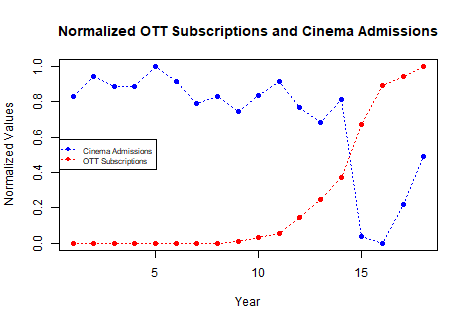
\includegraphics[width=0.8\linewidth]{plots/UCRCD_normalized-1}

Estimating initial parameters with Bass Model:

\begin{Shaded}
\begin{Highlighting}[]
\CommentTok{\# Cinema Admissions}
\NormalTok{BM.cinema\_admissions }\OtherTok{\textless{}{-}} \FunctionTok{BM}\NormalTok{(ott\_cinema\_annual}\SpecialCharTok{$}\NormalTok{cinema\_admissions, }\AttributeTok{display =}\NormalTok{ T)}
\end{Highlighting}
\end{Shaded}

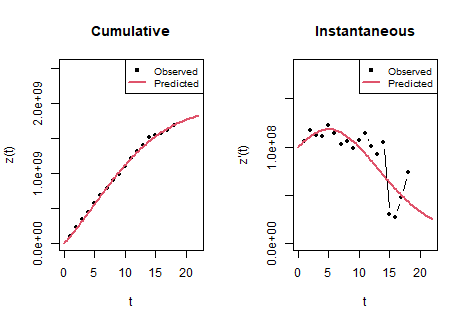
\includegraphics[width=0.8\linewidth]{plots/initial_UCRCD_bass-1}

\begin{Shaded}
\begin{Highlighting}[]
\NormalTok{m.c }\OtherTok{=}\NormalTok{ BM.cinema\_admissions}\SpecialCharTok{$}\NormalTok{Estimate[}\DecValTok{1}\NormalTok{, }\DecValTok{1}\NormalTok{]  }\CommentTok{\# Market potential for Cinema}
\NormalTok{p.c }\OtherTok{=}\NormalTok{ BM.cinema\_admissions}\SpecialCharTok{$}\NormalTok{Estimate[}\DecValTok{2}\NormalTok{, }\DecValTok{1}\NormalTok{]  }\CommentTok{\# Innovation coefficient for Cinema}
\NormalTok{q.c }\OtherTok{=}\NormalTok{ BM.cinema\_admissions}\SpecialCharTok{$}\NormalTok{Estimate[}\DecValTok{3}\NormalTok{, }\DecValTok{1}\NormalTok{]  }\CommentTok{\# Imitation coefficient for Cinema}

\CommentTok{\# OTT Subscriptions}
\NormalTok{BM.ott\_subscriptions }\OtherTok{\textless{}{-}} \FunctionTok{BM}\NormalTok{(ott\_cinema\_annual}\SpecialCharTok{$}\NormalTok{ott\_subscriptions\_M }\SpecialCharTok{*} \FloatTok{1e+06}\NormalTok{,}
    \AttributeTok{display =}\NormalTok{ T)}
\end{Highlighting}
\end{Shaded}

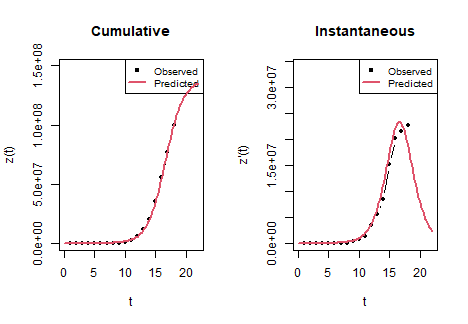
\includegraphics[width=0.8\linewidth]{plots/initial_UCRCD_bass-2}

\begin{Shaded}
\begin{Highlighting}[]
\NormalTok{m.o }\OtherTok{=}\NormalTok{ BM.ott\_subscriptions}\SpecialCharTok{$}\NormalTok{Estimate[}\DecValTok{1}\NormalTok{, }\DecValTok{1}\NormalTok{]  }\CommentTok{\# Market potential for OTT}
\NormalTok{p.o }\OtherTok{=}\NormalTok{ BM.ott\_subscriptions}\SpecialCharTok{$}\NormalTok{Estimate[}\DecValTok{2}\NormalTok{, }\DecValTok{1}\NormalTok{]  }\CommentTok{\# Innovation coefficient for OTT}
\NormalTok{q.o }\OtherTok{=}\NormalTok{ BM.ott\_subscriptions}\SpecialCharTok{$}\NormalTok{Estimate[}\DecValTok{3}\NormalTok{, }\DecValTok{1}\NormalTok{]  }\CommentTok{\# Imitation coefficient for OTT}
\end{Highlighting}
\end{Shaded}

GBM for cinema admissions:

\begin{Shaded}
\begin{Highlighting}[]
\CommentTok{\# Cinema Admissions GBM exponential shock}

\CommentTok{\# Define the time period when the COVID{-}19 shock begins}
\NormalTok{covid\_start }\OtherTok{\textless{}{-}} \DecValTok{2020} \SpecialCharTok{{-}} \DecValTok{2006} \SpecialCharTok{+} \DecValTok{1}

\CommentTok{\# m,p,q, a(starting point), b(memory of the shock), c(intensity)}
\NormalTok{GBM.cinema\_admissions }\OtherTok{\textless{}{-}} \FunctionTok{GBM}\NormalTok{(ott\_cinema\_annual}\SpecialCharTok{$}\NormalTok{cinema\_admissions, }\AttributeTok{shock =} \StringTok{"exp"}\NormalTok{,}
    \AttributeTok{nshock =} \DecValTok{1}\NormalTok{, }\AttributeTok{prelimestimates =} \FunctionTok{c}\NormalTok{(m.c, p.c, q.c, covid\_start, }\SpecialCharTok{{-}}\FloatTok{0.5}\NormalTok{, }\SpecialCharTok{{-}}\FloatTok{0.1}\NormalTok{))}
\end{Highlighting}
\end{Shaded}

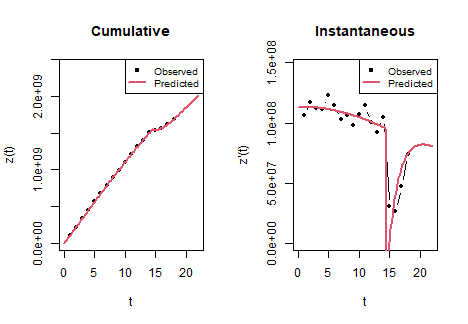
\includegraphics[width=0.8\linewidth]{plots/GBM_cinema_annual-1}

\begin{Shaded}
\begin{Highlighting}[]
\FunctionTok{summary}\NormalTok{(GBM.cinema\_admissions)}
\end{Highlighting}
\end{Shaded}

\begin{verbatim}
Call: ( Generalized Bass model with 1  Exponential  shock )

  GBM(series = ott_cinema_annual$cinema_admissions, shock = "exp", 
    nshock = 1, prelimestimates = c(m.c, p.c, q.c, covid_start, 
        -0.5, -0.1))

Residuals:
     Min.  1st Qu.   Median     Mean  3rd Qu.     Max. 
-8042512 -4373103    54956  -411703  2831777  9976519 

Coefficients:
           Estimate    Std.Error         Lower         Upper  p-value    
m     3.769432e+09 7.981598e+08  2.205067e+09  5.333796e+09 4.95e-04 ***
p     3.001909e-02 5.904782e-03  1.844593e-02  4.159225e-02 2.69e-04 ***
q     3.134837e-02 1.332680e-02  5.228311e-03  5.746842e-02 3.66e-02   *
a1    1.442851e+01 1.466754e-01  1.414103e+01  1.471599e+01 8.15e-19 ***
b1   -5.413931e-01 1.580551e-01 -8.511753e-01 -2.316109e-01 5.03e-03  **
c1   -1.319046e+00 2.390154e-01 -1.787508e+00 -8.505850e-01 1.32e-04 ***
---
 Signif. codes:  0 '***' 0.001 '**' 0.01 '*' 0.05 '.' 0.1 ' ' 1

 Residual standard error  5922966  on  12  degrees of freedom
 Multiple R-squared:   0.999907  Residual sum of squares:  4.209783e+14
\end{verbatim}

\begin{Shaded}
\begin{Highlighting}[]
\FunctionTok{checkresiduals}\NormalTok{(GBM.cinema\_admissions)}
\end{Highlighting}
\end{Shaded}

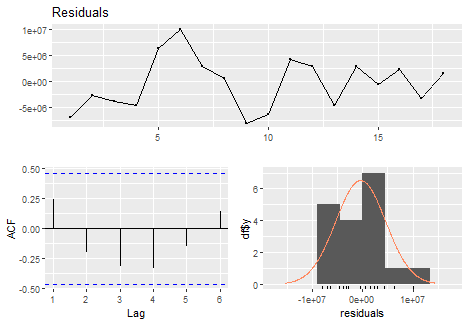
\includegraphics[width=0.8\linewidth]{plots/GBM_cinema_annual-2}

\begin{verbatim}

    Ljung-Box test

data:  Residuals
Q* = 7.3266, df = 4, p-value = 0.1196

Model df: 0.   Total lags used: 4
\end{verbatim}

\begin{Shaded}
\begin{Highlighting}[]
\NormalTok{m.c }\OtherTok{=}\NormalTok{ BM.cinema\_admissions}\SpecialCharTok{$}\NormalTok{Estimate[}\DecValTok{1}\NormalTok{, }\DecValTok{1}\NormalTok{]  }\CommentTok{\# Market potential for Cinema}
\NormalTok{p.c }\OtherTok{=}\NormalTok{ BM.cinema\_admissions}\SpecialCharTok{$}\NormalTok{Estimate[}\DecValTok{2}\NormalTok{, }\DecValTok{1}\NormalTok{]  }\CommentTok{\# Innovation coefficient for Cinema}
\NormalTok{q.c }\OtherTok{=}\NormalTok{ BM.cinema\_admissions}\SpecialCharTok{$}\NormalTok{Estimate[}\DecValTok{3}\NormalTok{, }\DecValTok{1}\NormalTok{]  }\CommentTok{\# Imitation coefficient for Cinema}
\end{Highlighting}
\end{Shaded}

GGM for OTT subscriptions:

\begin{Shaded}
\begin{Highlighting}[]
\NormalTok{GGM.ott\_subscriptions }\OtherTok{\textless{}{-}} \FunctionTok{GGM}\NormalTok{(ott\_cinema\_annual}\SpecialCharTok{$}\NormalTok{ott\_subscriptions\_M }\SpecialCharTok{*} \FloatTok{1e+06}\NormalTok{,}
    \AttributeTok{prelimestimates =} \FunctionTok{c}\NormalTok{(m.o, }\FloatTok{0.01}\NormalTok{, }\FloatTok{0.01}\NormalTok{, p.o, q.o), }\AttributeTok{oos =} \DecValTok{10}\NormalTok{)}
\end{Highlighting}
\end{Shaded}

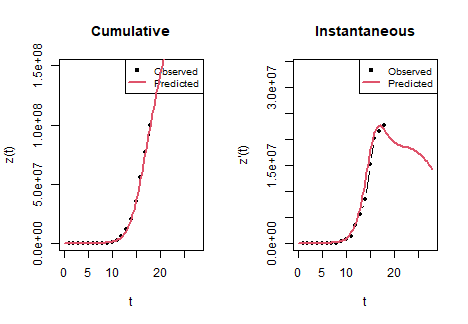
\includegraphics[width=0.8\linewidth]{plots/GGM_ott_annual-1}

\begin{Shaded}
\begin{Highlighting}[]
\FunctionTok{summary}\NormalTok{(GGM.ott\_subscriptions)}
\end{Highlighting}
\end{Shaded}

\begin{verbatim}
Call: ( Guseo Guidolin Model )

  GGM(series = ott_cinema_annual$ott_subscriptions_M * 1e+06, prelimestimates = c(m.o, 
    0.01, 0.01, p.o, q.o), oos = 10)

Residuals:
      Min.   1st Qu.    Median      Mean   3rd Qu.      Max. 
-565793.3 -200245.4  -37475.4  -35995.0    -529.7  513439.9 

Coefficients:
          Estimate    Std.Error         Lower        Upper  p-value    
K    3.637506e+08 2.583308e+09 -4.699440e+09 5.426941e+09 8.90e-01    
pc   3.338036e-04 3.137188e-03 -5.814972e-03 6.482580e-03 9.17e-01    
qc   2.507607e-01 4.863858e-01 -7.025380e-01 1.204059e+00 6.15e-01    
ps   2.875537e-05 5.550260e-05 -8.002772e-05 1.375385e-04 6.13e-01    
qs   6.468712e-01 1.167683e-01  4.180094e-01 8.757330e-01 9.55e-05 ***
---
 Signif. codes:  0 '***' 0.001 '**' 0.01 '*' 0.05 '.' 0.1 ' ' 1

 Residual standard error  314048.1  on  13  degrees of freedom
 Multiple R-squared:   0.999917  Residual sum of squares:  1.282141e+12
\end{verbatim}

\begin{Shaded}
\begin{Highlighting}[]
\FunctionTok{checkresiduals}\NormalTok{(GGM.ott\_subscriptions)}
\end{Highlighting}
\end{Shaded}

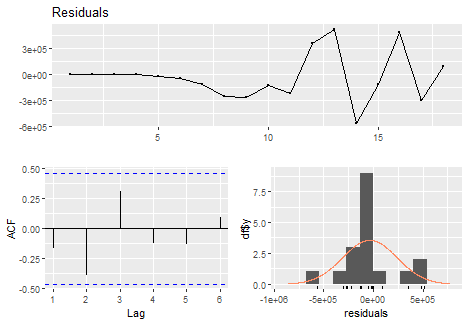
\includegraphics[width=0.8\linewidth]{plots/GGM_ott_annual-2}

\begin{verbatim}

    Ljung-Box test

data:  Residuals
Q* = 6.6661, df = 4, p-value = 0.1546

Model df: 0.   Total lags used: 4
\end{verbatim}

\begin{Shaded}
\begin{Highlighting}[]
\DocumentationTok{\#\#\#estimate the UCRCD (with delta and gamma)}
\NormalTok{UCRCD.adm.subs}\OtherTok{\textless{}{-}} \FunctionTok{UCRCD}\NormalTok{(}
  \AttributeTok{series1 =}\NormalTok{ ott\_cinema\_annual}\SpecialCharTok{$}\NormalTok{cinema\_admissions,  }\CommentTok{\# Instantaneous cinema admissions}
  \AttributeTok{series2 =}\NormalTok{ ott\_cinema\_annual}\SpecialCharTok{$}\NormalTok{ott\_subscriptions\_M}\SpecialCharTok{*}\FloatTok{1e6}\NormalTok{,  }\CommentTok{\# Instantaneous OTT subscriptions}
  \AttributeTok{m1 =}\NormalTok{ m.c,                    }\CommentTok{\# Market potential for cinema (GBM result)}
  \AttributeTok{p1c =}\NormalTok{ p.c,                   }\CommentTok{\# Innovation coefficient for cinema}
  \AttributeTok{q1c =}\NormalTok{ q.c,                   }\CommentTok{\# Imitation coefficient for cinema}
  \AttributeTok{m2 =}\NormalTok{ m.o,                    }\CommentTok{\# Market potential for OTT (BM result)}
  \AttributeTok{p2 =}\NormalTok{ p.o,                   }\CommentTok{\# Innovation coefficient for OTT}
  \AttributeTok{q2 =}\NormalTok{ q.o                    }\CommentTok{\# Imitation coefficient for OTT}
\NormalTok{)}
\end{Highlighting}
\end{Shaded}

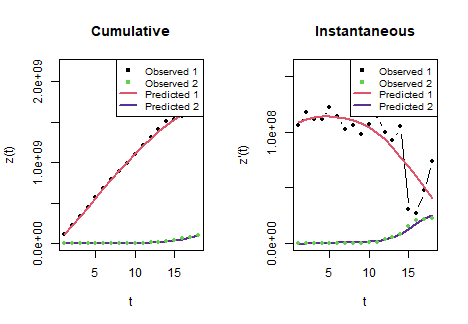
\includegraphics[width=0.8\linewidth]{plots/UCRCD-1}

\begin{Shaded}
\begin{Highlighting}[]
\FunctionTok{summary}\NormalTok{(UCRCD.adm.subs)}
\end{Highlighting}
\end{Shaded}

\begin{verbatim}
Call: ( UCRCD Model )

  UCRCD(series1 = ott_cinema_annual$cinema_admissions, series2 = ott_cinema_annual$ott_subscriptions_M * 
    1e+06, m1 = m.c, m2 = m.o, p1c = p.c, q1c = q.c, p2 = p.o, 
    q2 = q.o)

Residuals Series 1:
      Min.   1st Qu.    Median      Mean   3rd Qu.      Max. 
-39075071  -3849539   -244580    117494   6788756  33668234 

Residuals Series 2:
     Min.  1st Qu.   Median     Mean  3rd Qu.     Max. 
-2575467  -650131  -179424    21790   371339  3077838 

Coefficients:
            Estimate    Std.Error         Lower        Upper  p-value    
mc     2.495088e+09 5.878604e+08  1.342903e+09 3.647273e+09 2.05e-04 ***
p1c    4.255135e-02 7.721923e-03  2.741666e-02 5.768604e-02 6.15e-06 ***
p2    -3.738760e-04 3.905354e-03 -8.028230e-03 7.280478e-03 9.24e-01    
q1c   -8.770799e-01 5.305156e-01 -1.916871e+00 1.627115e-01 1.09e-01    
q2     8.680689e-01 6.183658e-01 -3.439058e-01 2.080044e+00 1.71e-01    
delta  9.504870e-01 5.105348e-01 -5.014288e-02 1.951117e+00 7.28e-02   .
gamma  8.657815e-01 6.244519e-01 -3.581218e-01 2.089685e+00 1.76e-01    
---
 Signif. codes:  0 '***' 0.001 '**' 0.01 '*' 0.05 '.' 0.1 ' ' 1

 Residual standard error Series 1: 21744888  on  11  degrees of freedom
 Residual standard error Series 2: 1572385  on  11  degrees of freedom
 Multiple R-squared:   0.939158  Residual sum of squares:  5.228438e+15
\end{verbatim}

!!! TODO: SINCE THERE IS A SCALE DIFFERENCE IN THE DATA, THE PLOT DOESNT
EXPLAIN MUCH. CAN I WORK WITH NORMALIZED DATA WHEN MODELING UCRCD? Will
it be academically acceptable? Let's try:

\begin{Shaded}
\begin{Highlighting}[]
\CommentTok{\# Cinema Admissions}
\NormalTok{BM.cinema\_admissions.norm }\OtherTok{\textless{}{-}} \FunctionTok{BM}\NormalTok{(cinema\_admissions.norm, }\AttributeTok{display =}\NormalTok{ T)}
\end{Highlighting}
\end{Shaded}

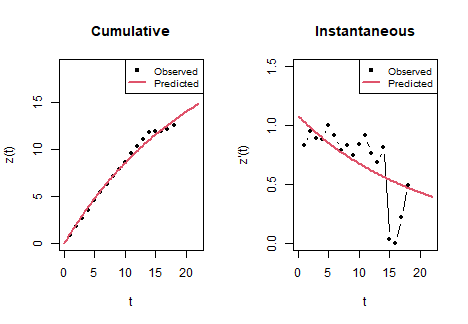
\includegraphics[width=0.8\linewidth]{plots/initial_UCRCD_bass_norm-1}

\begin{Shaded}
\begin{Highlighting}[]
\NormalTok{m.c }\OtherTok{=}\NormalTok{ BM.cinema\_admissions.norm}\SpecialCharTok{$}\NormalTok{Estimate[}\DecValTok{1}\NormalTok{, }\DecValTok{1}\NormalTok{]  }\CommentTok{\# Market potential for Cinema}
\NormalTok{p.c }\OtherTok{=}\NormalTok{ BM.cinema\_admissions.norm}\SpecialCharTok{$}\NormalTok{Estimate[}\DecValTok{2}\NormalTok{, }\DecValTok{1}\NormalTok{]  }\CommentTok{\# Innovation coefficient for Cinema}
\NormalTok{q.c }\OtherTok{=}\NormalTok{ BM.cinema\_admissions.norm}\SpecialCharTok{$}\NormalTok{Estimate[}\DecValTok{3}\NormalTok{, }\DecValTok{1}\NormalTok{]  }\CommentTok{\# Imitation coefficient for Cinema}

\CommentTok{\# OTT Subscriptions}
\NormalTok{BM.ott\_subscriptions.norm }\OtherTok{\textless{}{-}} \FunctionTok{BM}\NormalTok{(ott\_subscriptions.norm, }\AttributeTok{display =}\NormalTok{ T)}
\end{Highlighting}
\end{Shaded}

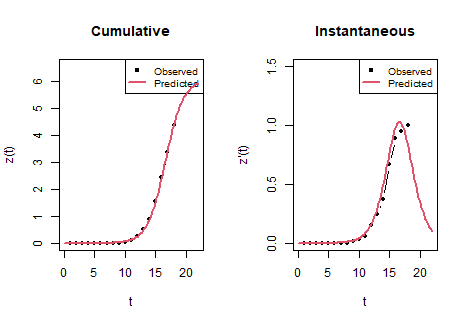
\includegraphics[width=0.8\linewidth]{plots/initial_UCRCD_bass_norm-2}

\begin{Shaded}
\begin{Highlighting}[]
\NormalTok{m.o }\OtherTok{=}\NormalTok{ BM.ott\_subscriptions.norm}\SpecialCharTok{$}\NormalTok{Estimate[}\DecValTok{1}\NormalTok{, }\DecValTok{1}\NormalTok{]  }\CommentTok{\# Market potential for OTT}
\NormalTok{p.o }\OtherTok{=}\NormalTok{ BM.ott\_subscriptions.norm}\SpecialCharTok{$}\NormalTok{Estimate[}\DecValTok{2}\NormalTok{, }\DecValTok{1}\NormalTok{]  }\CommentTok{\# Innovation coefficient for OTT}
\NormalTok{q.o }\OtherTok{=}\NormalTok{ BM.ott\_subscriptions.norm}\SpecialCharTok{$}\NormalTok{Estimate[}\DecValTok{3}\NormalTok{, }\DecValTok{1}\NormalTok{]  }\CommentTok{\# Imitation coefficient for OTT}
\end{Highlighting}
\end{Shaded}

GBM for cinema admissions:

\begin{Shaded}
\begin{Highlighting}[]
\CommentTok{\# Cinema Admissions GBM exponential shock}

\CommentTok{\# Define the time period when the COVID{-}19 shock begins}
\NormalTok{covid\_start }\OtherTok{\textless{}{-}} \DecValTok{2020} \SpecialCharTok{{-}} \DecValTok{2006} \SpecialCharTok{+} \DecValTok{1}

\CommentTok{\# m,p,q, a(starting point), b(memory of the shock), c(intensity)}
\NormalTok{GBM.cinema\_admissions.norm }\OtherTok{\textless{}{-}} \FunctionTok{GBM}\NormalTok{(cinema\_admissions.norm, }\AttributeTok{shock =} \StringTok{"exp"}\NormalTok{,}
    \AttributeTok{nshock =} \DecValTok{1}\NormalTok{, }\AttributeTok{prelimestimates =} \FunctionTok{c}\NormalTok{(m.c, p.c, q.c, covid\_start, }\SpecialCharTok{{-}}\FloatTok{0.5}\NormalTok{, }\SpecialCharTok{{-}}\FloatTok{0.1}\NormalTok{))}
\end{Highlighting}
\end{Shaded}

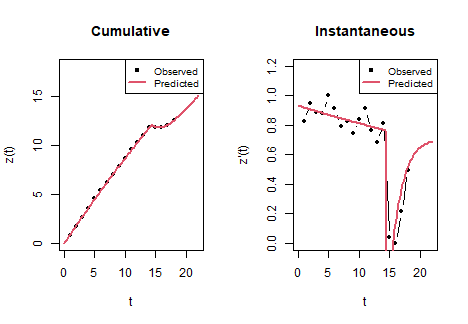
\includegraphics[width=0.8\linewidth]{plots/GBM_cinema_annual_norm-1}

\begin{Shaded}
\begin{Highlighting}[]
\FunctionTok{summary}\NormalTok{(GBM.cinema\_admissions.norm)}
\end{Highlighting}
\end{Shaded}

\begin{verbatim}
Call: ( Generalized Bass model with 1  Exponential  shock )

  GBM(series = cinema_admissions.norm, shock = "exp", nshock = 1, 
    prelimestimates = c(m.c, p.c, q.c, covid_start, -0.5, -0.1))

Residuals:
      Min.   1st Qu.    Median      Mean   3rd Qu.      Max. 
-0.096358 -0.057368 -0.011294 -0.008509  0.035628  0.098147 

Coefficients:
           Estimate    Std.Error         Lower         Upper  p-value    
m    581.878081928 3.033552e+04 -5.887465e+04 60038.4067906 9.85e-01    
p      0.001599336 8.411980e-02 -1.632724e-01     0.1664711 9.85e-01    
q     -0.012431924 7.304014e-02 -1.555880e-01     0.1307241 8.68e-01    
a1    14.357728896 1.620019e-01  1.404021e+01    14.6752467 2.84e-18 ***
b1    -0.464933344 1.442744e-01 -7.477059e-01    -0.1821608 7.32e-03  **
c1    -1.743752639 3.255658e-01 -2.381850e+00    -1.1056555 1.72e-04 ***
---
 Signif. codes:  0 '***' 0.001 '**' 0.01 '*' 0.05 '.' 0.1 ' ' 1

 Residual standard error  0.068219  on  12  degrees of freedom
 Multiple R-squared:   0.999785  Residual sum of squares:  0.055846
\end{verbatim}

\begin{Shaded}
\begin{Highlighting}[]
\FunctionTok{checkresiduals}\NormalTok{(GBM.cinema\_admissions.norm)}
\end{Highlighting}
\end{Shaded}

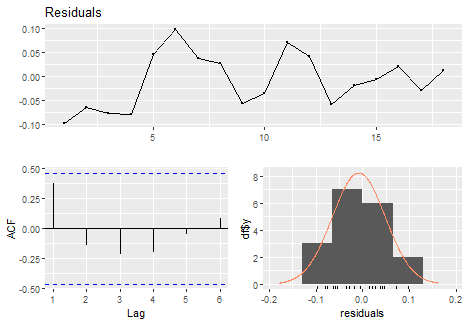
\includegraphics[width=0.8\linewidth]{plots/GBM_cinema_annual_norm-2}

\begin{verbatim}

    Ljung-Box test

data:  Residuals
Q* = 5.5125, df = 4, p-value = 0.2386

Model df: 0.   Total lags used: 4
\end{verbatim}

\begin{Shaded}
\begin{Highlighting}[]
\NormalTok{m.c }\OtherTok{=}\NormalTok{ BM.cinema\_admissions.norm}\SpecialCharTok{$}\NormalTok{Estimate[}\DecValTok{1}\NormalTok{, }\DecValTok{1}\NormalTok{]  }\CommentTok{\# Market potential for Cinema}
\NormalTok{p.c }\OtherTok{=}\NormalTok{ BM.cinema\_admissions.norm}\SpecialCharTok{$}\NormalTok{Estimate[}\DecValTok{2}\NormalTok{, }\DecValTok{1}\NormalTok{]  }\CommentTok{\# Innovation coefficient for Cinema}
\NormalTok{q.c }\OtherTok{=}\NormalTok{ BM.cinema\_admissions.norm}\SpecialCharTok{$}\NormalTok{Estimate[}\DecValTok{3}\NormalTok{, }\DecValTok{1}\NormalTok{]  }\CommentTok{\# Imitation coefficient for Cinema}
\end{Highlighting}
\end{Shaded}

GGM for OTT subscriptions:

\begin{Shaded}
\begin{Highlighting}[]
\NormalTok{GGM.ott\_subscriptions.norm }\OtherTok{\textless{}{-}} \FunctionTok{GGM}\NormalTok{(ott\_subscriptions.norm, }\AttributeTok{prelimestimates =} \FunctionTok{c}\NormalTok{(m.o,}
    \FloatTok{0.01}\NormalTok{, }\FloatTok{0.01}\NormalTok{, p.o, q.o), }\AttributeTok{oos =} \DecValTok{10}\NormalTok{)}
\end{Highlighting}
\end{Shaded}

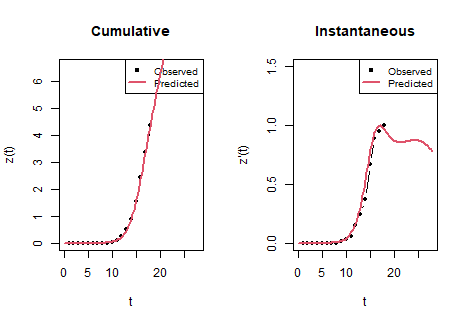
\includegraphics[width=0.8\linewidth]{plots/GGM_ott_annual_norm-1}

\begin{Shaded}
\begin{Highlighting}[]
\FunctionTok{summary}\NormalTok{(GGM.ott\_subscriptions.norm)}
\end{Highlighting}
\end{Shaded}

\begin{verbatim}
Call: ( Guseo Guidolin Model )

  GGM(series = ott_subscriptions.norm, prelimestimates = c(m.o, 
    0.01, 0.01, p.o, q.o), oos = 10)

Residuals:
       Min.    1st Qu.     Median       Mean    3rd Qu.       Max. 
-2.478e-02 -8.823e-03 -1.650e-03 -1.613e-03 -2.339e-05  2.257e-02 

Coefficients:
          Estimate    Std.Error         Lower        Upper  p-value    
K    1.822034e+01 1.813083e+02 -3.371374e+02 3.735781e+02 9.21e-01    
pc   2.753476e-04 4.188104e-03 -7.933185e-03 8.483880e-03 9.49e-01    
qc   2.436747e-01 4.896156e-01 -7.159542e-01 1.203304e+00 6.27e-01    
ps   2.795305e-05 5.303582e-05 -7.599524e-05 1.319013e-04 6.07e-01    
qs   6.486660e-01 1.148359e-01  4.235917e-01 8.737403e-01 7.95e-05 ***
---
 Signif. codes:  0 '***' 0.001 '**' 0.01 '*' 0.05 '.' 0.1 ' ' 1

 Residual standard error  0.013758  on  13  degrees of freedom
 Multiple R-squared:   0.999917  Residual sum of squares:  0.002461
\end{verbatim}

\begin{Shaded}
\begin{Highlighting}[]
\FunctionTok{checkresiduals}\NormalTok{(GGM.ott\_subscriptions.norm)}
\end{Highlighting}
\end{Shaded}

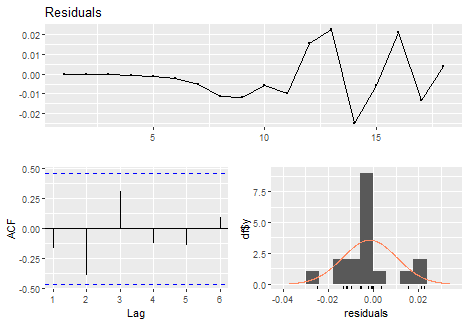
\includegraphics[width=0.8\linewidth]{plots/GGM_ott_annual_norm-2}

\begin{verbatim}

    Ljung-Box test

data:  Residuals
Q* = 6.655, df = 4, p-value = 0.1553

Model df: 0.   Total lags used: 4
\end{verbatim}

\begin{Shaded}
\begin{Highlighting}[]
\DocumentationTok{\#\#\#estimate the UCRCD (with delta and gamma)}
\NormalTok{UCRCD.adm.subs.norm}\OtherTok{\textless{}{-}} \FunctionTok{UCRCD}\NormalTok{(}
  \AttributeTok{series1 =}\NormalTok{ cinema\_admissions.norm,  }\CommentTok{\# Instantaneous cinema admissions}
  \AttributeTok{series2 =}\NormalTok{ ott\_subscriptions.norm,  }\CommentTok{\# Instantaneous OTT subscriptions}
  \AttributeTok{m1 =}\NormalTok{ m.c,                    }\CommentTok{\# Market potential for cinema (GBM result)}
  \AttributeTok{p1c =}\NormalTok{ p.c,                   }\CommentTok{\# Innovation coefficient for cinema}
  \AttributeTok{q1c =}\NormalTok{ q.c,                   }\CommentTok{\# Imitation coefficient for cinema}
  \AttributeTok{m2 =}\NormalTok{ m.o,                    }\CommentTok{\# Market potential for OTT (BM result)}
  \AttributeTok{p2 =}\NormalTok{ p.o,                   }\CommentTok{\# Innovation coefficient for OTT}
  \AttributeTok{q2 =}\NormalTok{ q.o                    }\CommentTok{\# Imitation coefficient for OTT}
\NormalTok{)}
\end{Highlighting}
\end{Shaded}

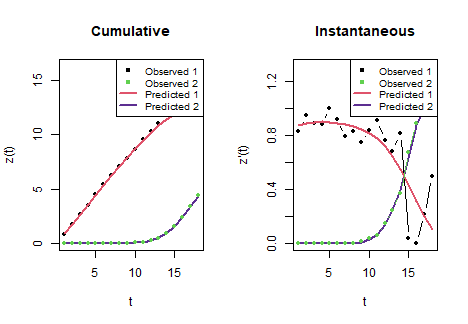
\includegraphics[width=0.8\linewidth]{plots/UCRCD_norm-1}

\begin{Shaded}
\begin{Highlighting}[]
\FunctionTok{summary}\NormalTok{(UCRCD.adm.subs.norm)}
\end{Highlighting}
\end{Shaded}

\begin{verbatim}
Call: ( UCRCD Model )

  UCRCD(series1 = cinema_admissions.norm, series2 = ott_subscriptions.norm, 
    m1 = m.c, m2 = m.o, p1c = p.c, q1c = q.c, p2 = p.o, q2 = q.o)

Residuals Series 1:
      Min.   1st Qu.    Median      Mean   3rd Qu.      Max. 
-0.400803 -0.045457  0.020390  0.005014  0.053529  0.392080 

Residuals Series 2:
       Min.    1st Qu.     Median       Mean    3rd Qu.       Max. 
-6.585e-02 -1.153e-03 -3.615e-05  2.162e-04  2.489e-03  4.263e-02 

Coefficients:
            Estimate   Std.Error        Lower       Upper  p-value    
mc     2.113772e+01 1.858348987 17.495421293 24.78001546 3.29e-12 ***
p1c    4.068835e-02 0.005394613  0.030115108  0.05126160 2.58e-08 ***
p2    -6.260099e-05 0.004807900 -0.009485912  0.00936071 9.90e-01    
q1c   -2.589281e-01 0.105988731 -0.466662199 -0.05119401 2.09e-02   *
q2     1.110295e+00 0.310919900  0.500902930  1.71968654 1.26e-03  **
delta  3.210642e-01 0.114933126  0.095799415  0.54632899 9.14e-03  **
gamma  1.109853e+00 0.320895724  0.480908569  1.73879669 1.70e-03  **
---
 Signif. codes:  0 '***' 0.001 '**' 0.01 '*' 0.05 '.' 0.1 ' ' 1

 Residual standard error Series 1: 0.222172  on  11  degrees of freedom
 Residual standard error Series 2: 0.027163  on  11  degrees of freedom
 Multiple R-squared:   0.904185  Residual sum of squares:  0.55108
\end{verbatim}

\end{document}
